\documentclass[11pt,titlepage,listof=totoc,bibliography=totoc,twoside]{scrreprt}

%%%%%%%%%%%%%%%%%%%%%%%%%%%%%%%%%%%%%%%%%%%%%%%%%%%%%%%%%%%%%%%%%%%%%%%%%%%%%%%%%%%%%%%%%%%%%%%
%
% Packages

	%\usepackage[latin1,ansinew]{inputenc}			% für arbeiten unter WINDOWS, Umlaute
	\usepackage[utf8]{inputenc}					% für arbeiten unter UNIX, Umlaute
	\usepackage[T1]{fontenc}
	\usepackage[ngerman]{babel}
	% 	\usepackage{ngerman}
 	\usepackage{a4wide}						% a4wide is obsolete, use geometry-package instead
	% 	\usepackage{geometry}
	% 	\geometry{a4paper,twoside,left=40mm,right=30mm,top=2cm,bottom=2cm}
	\usepackage{charter}					% Schriftart setzen
	\usepackage{graphicx}					% Bilder einbinden
	\usepackage[fleqn]{amsmath}				% schöner Mathekrempel, fleqn wird bei Aufruf im Header automatisch angefordert
	\usepackage{amsfonts}
	\usepackage{amssymb}
 	\usepackage{color}					% bunt
	\usepackage{fancyhdr}					% Kopf- und Fußzeile
% 	\usepackage{scrlayer-scrpage}
	\usepackage{ifpdf}					% Bereiche, welche nur beim Kompilieren mit pdf-Latex übersetzt werden sollen
	\usepackage[normalem]{ulem}				% Unterstreichungen
 	\usepackage{booktabs}					% für schöne Tabellen mit schönen hoizontalen Linien und konsistenten vertikalen Abständen
 	\usepackage{subfigure}
 	\usepackage{multirow}
 	\usepackage{type1cm,eso-pic}
	\usepackage{tabularx}
	\usepackage{units}					% für schöne Brüche und schräge Einheiten
	\usepackage{dcolumn}					% für Ausrichtungen von Tabellenspalten am Dezimaltrenner
	\usepackage{ifthen}
	\usepackage[version=3]{mhchem}
	\usepackage{lscape}
	\usepackage{varwidth}					% für resizebox um formeln
	\usepackage{listings}
	\usepackage{dirtree}
	
	\PassOptionsToPackage{hyphens}{url}			% Umbrüche nach ``-'' erlauben, muss vor hyperref stehen !!!
	\usepackage[
		colorlinks=false,
		breaklinks=true,
		pdfborder={0 0 0},
		pdfstartview=Fit,				% startet mit Ganzseitenanzeige
		pdfsubject={FiPPS Programmdokumentation},
		pdftitle={FiPPS Programmdokumentation},
		pdfauthor={Andreas Hauffe}
	]{hyperref}						% Verlinkungen, unbedingt als letztes Paket laden ! damit keine internen Einstellungen des Paketes überschrieben werden können

	\pdfcompresslevel=9					% beste Kompression
	
% Nutzeroptionen input
	
	\newboolean{interneVersion}
	\setboolean{interneVersion}{true}


% Einstellungen
	
	% URLs richtig umbrechen
	 
	\makeatletter
	\g@addto@macro\UrlBreaks{
	  \do\a\do\b\do\c\do\d\do\e\do\f\do\g\do\h\do\i\do\j
	  \do\k\do\l\do\m\do\n\do\o\do\p\do\q\do\r\do\s\do\t
	  \do\u\do\v\do\w\do\x\do\y\do\z\do\&\do\1\do\2\do\3
	  \do\4\do\5\do\6\do\7\do\8\do\9\do\0}
	\g@addto@macro\UrlSpecials{\do\/{\mbox{\UrlFont/}\hskip 0pt plus 1pt}}
	\makeatother
	
	% Längen
	
% 	\setlength{\textheight}{24.5cm}
% 	\setlength{\textwidth}{16cm}
% 	\setlength{\evensidemargin}{0mm}
% 	\setlength{\oddsidemargin}{0mm}
	
	\setlength{\parindent}{0mm}
% 	\setlength{\parskip}{2mm}
	\setlength{\parskip}{1ex plus0.5ex minus0.5ex}
	\setlength{\partopsep}{0mm}

	% Überschriftengestaltung

	\setkomafont{sectioning}{\bfseries}	% Überschriften fett
% 	\setkomafont{sectioning}{\mdseries}	% Überschriften normal
	\addtokomafont{caption}{\small}
	\setkomafont{captionlabel}{\textbf}
	\addtokomafont{paragraph}{\normalfont}	% Paragraph normal (nicht fett)
	
	\renewcommand{\baselinestretch}{1.0}
	
	% Pagestyle
	
	% Festlegung des Seitenstils (fancyhdr)
	\pagestyle{fancy}
	\fancyhf{}
	\fancyhead[LE,RO]{\thepage}
	% 	\fancyfoot[LO]{}
	% 	\fancyfoot[RE]{Institut}
	% 	\fancyhead[RE]{eLamX User Guide}
	% 	\fancyhead[LO]{eLamX User Guide}
	\fancyhead[RE]{FiPPS Programmdokumentation}
	\fancyhead[LO]{FiPPS Programmdokumentation}
	\renewcommand{\headrulewidth}{0.5pt}
	% 	\renewcommand{\footrulewidth}{0.5pt}
	
	% subfigure ohne Nummer bzw. Buchstaben
	
	\makeatletter
	\renewcommand{\@thesubfigure}{}
	\makeatother

	% Counter
	\newcommand{\IVzTiefe}{2}
	\setcounter{MaxMatrixCols}{12}		% maximale Matrixgröße
	\setcounter{secnumdepth}{\IVzTiefe+1}		% bis subsubsection (Gliederungsebene 3) durchnummerieren
						% andere Gliederungsebenen:
						% -1 part	1 section	3 subsubsection		5 subparagraph
						% 0 chapter	2 subsection	4 paragraph
	\setcounter{tocdepth}{\IVzTiefe}		% analog secnumdepth
	
	% Draft- Wasserzeichen
	
	\makeatletter
	\AddToShipoutPicture{%
	\setlength{\@tempdimb}{.5\paperwidth}%
	\setlength{\@tempdimc}{.5\paperheight}%
	\setlength{\unitlength}{1pt}%
	\put(\strip@pt\@tempdimb,\strip@pt\@tempdimc){%
	\makebox(0,0){\rotatebox{45}{\textcolor[gray]{0.75}%
	{\fontsize{3cm}{3cm}\selectfont{Draft}}}}%
  % 	\makebox(-100,-300){\rotatebox{45}{\textcolor[gray]{0.95}%
  % 	{\fontsize{2cm}{2cm}\selectfont{Internal Use}}}}
	\makebox(-500,-0){\rotatebox{90}{\textcolor[gray]{0.75}%
	{\fontsize{0.7cm}{0.7cm}\selectfont{Draft \textcopyright\ GPL-3.0 license 2025 - LFT, ILR, TU Dresden}}}}
	}%
	}
	\makeatother

	% lokale Einrückung
	
	% \begin{indenting}{linker rand}{rechter rand}{label}   
	% \end{indenting}
	
	\newenvironment{indenting}[3]%
	{\begin{list}{#3}{\setlength{\leftmargin}{#1}%
	\setlength{\labelwidth}{#1}%
	\setlength{\rightmargin}{#2}%
	\setlength{\topsep}{0pt}%
	\setlength{\partopsep}{0pt}%
	\setlength{\parskip}{0pt}%
	\setlength{\parsep}{0pt}%
	\setlength{\itemsep}{0pt}%
	} \item\relax }%
	{\end{list}}
	
	% Tabellenspalte mit fester Breite und zentrierter Textausrichtung
	
% 	\newcolumntype{C}[1]{>{\centering\arraybackslash}p{#1}} % zentrierte Spalten mit Breitenangabe
% 	\newcolumntype{C}{>{\bfseries\centering\arraybackslash}X}
	\newcolumntype{C}{>{\centering\arraybackslash}X}	

	% Benutzerdefinierte Befehle
	\newcommand{\transpose}{^\textsf{T}}	

\begin{document}

	% Tabellenspalten
% Textausrichtung bei fester Spaltenbreite

% Verwendet man in der Tabellendefinition die Option p{}, so wird der Text innerhalb der Spalten automatisch linksbündig ausgerichtet. Leider blockiert das p{} die Ausrichtungsoptionen c und r. Möchte man trotz angegebener Spaltenbreite eine Textausrichtung mitdefinieren, muss folgendes in die Präambel geschrieben werden:

% \usepackage{tabularx}
% \newcolumntype{C}[1]{>{\centering\arraybackslash}p{#1}} % zentrierte Spalten mit Breitenangabe 
% \newcolumntype{R}[1]{>{\raggedleft\arraybackslash}p{#1}} % rechtsbündig mit Breitenangabe 

% Jetzt kann man an Stelle des p{BREITE} einfach C{BREITE} für zentrierte, und R{BREITE} für rechtsbündige Textausrichtung verwenden.

% Soll innerhalb einer einzelnen Spalte eine andere Textausrichtung als die vordefinierte gesetzt werden, muss folgendes in die Präambel geschrieben werden:

% \newcommand{\ctab}{\centering\arraybackslash } % Tabellenabschnitt zentrieren 
% \newcommand{\rtab}{\raggedleft\arraybackslash} % Tabellenabschnitt rechtsbündig 
% \newcommand{\ltab}{\raggedright\arraybackslash} % Tabellenabschnitt linksbündig 

	% hier werden noch ein paar Abstände umdefiniert, damit der Abstand oberhalb von Formeln nicht so riesig wird.

	\abovedisplayskip=0pt plus 6pt minus 6pt
	\abovedisplayshortskip=0pt plus 3pt
	\belowdisplayskip=14pt plus 3pt minus 9pt
	\belowdisplayshortskip=7pt plus 3pt minus 4pt

\begin{titlepage}
	\enlargethispage{1cm}
	\newlength{\logoheight}\settoheight{\logoheight}{
\includegraphics[width=57mm]{Logo/TU_Logo_SW}}
	
\includegraphics[width=57mm]{Logo/TU_Logo_SW}	\hfill	
\includegraphics[height=\logoheight]{Logo/ILR_Logo_redone}\\[1cm]
	
	\centering
	\huge
	\textsc{Technische Universität Dresden}

	\bigskip
	\Large
	\textsc{Fakultät Maschinenwesen\\
	Institut für Luft- und Raumfahrttechnik\\
	Professur für Luftfahrzeugtechnik\\
	Prof. Dr. J. Markmiller}
    
	\vspace{2.5cm}
	\centering
	\huge
	FiPPS\\[0.5cm]
	
	\Large
	\huge
	Programmdokumentation\\[0.5cm]
	\Large
	\today\\[0.5cm]
	(FiPPS-Version 2.0.0 Rev. 474)
	\normalsize
	\vfill
	\begin{tabular}{ll@{\qquad}r}
	Autor:	&	Andreas Hauffe  & 	\url{andreas.hauffe@tu-dresden.de} \\
		    &	Florian Dexl	& 	\url{florian.dexl@tu-dresden.de} \\
		    &	Martin Rädel	&	 \\
	\end{tabular}
	
\end{titlepage}

\setcounter{page}{1}

\pagenumbering{roman}

\tableofcontents

\newpage

\setcounter{page}{1}

\pagenumbering{arabic}

\chapter{Allgemeine Hinweise}

FiPPS\textsuperscript{2} ist grundsätzlich für den Gebrauch in automatischen Prozessen entwickelt worden. Aus diesem Grund sind die Eingabeformate stark für das Einlesen mit Fortranprogrammen optimiert, was Einschränkungen bei der Menschenlesbarkeit zur Folge hat. Dabei ist der Input auch stark mit der Vernetzungsbibliothek ``FEModeller'' verbunden. Diese kann alle aktuellen Fähigkeiten von FiPPS\textsuperscript{2} ansprechen und stellt somit die einfachste Art dar, um die FiPPS\textsuperscript{2}-Eingabedateien zu erstellen.

\section{Pivotelemente der Steifigkeitsmatrix}

Um Elemente mit rotatorischen Freiheitsgraden (Beam2, Quad8) mit Elementen ohne rotatische Freiheitsgrade (Lsolid20) korrekt verbinden zu können, wird vor dem Lösen des Gleichungssystems die Elementsteifigkeitsmatrix auf Nulleinträge der Pivotelemente geprüft. Vorhandene Nulleinträge werden durch die Norm der Elementsteifigkeitsmatrix ersetzt, sodass ein lösbares Gleichungssystem erhalten wird. Eine Prüfung auf eventuell vorhandene freie Knoten erfolgt dabei nicht. Die Prüfung und das Ersetzen der Pivotelemente erfolgt in MUMPS über die Option \emph{ICNTL(24)}.

\section{linear statische Rechnung}

\section{Beulrechnung}

\section{Fluid-Strukturkopplung}
\label{sec:fluid-strukturkopplung}

In FiPPS\textsuperscript{2} sind aktuell zwei Arten der Fluid-Strukturkopplung implementiert, eine 2D-Kopplung (xfoil, Panel2D) für Berechnungen an Profilen und eine 3D-Kopplung (APAME) für Flügelsimulationen. In beiden Fällen werden die aerodynamischen Rechnungen auf Basis der Potentialtheorie ausschließlich dafür genutzt, um aerodynamische Lasten auf die Struktur zur generieren. Die sich daraus ergebende Strukturverformungen beeinflussen das Strömungsverhalten. Es handelt sich bei diesen Rechnungen infolgedessen um iterative numerische Methoden. 

Da es sich im Sinne der Struktursimulation um reine Lasten handelt, wird die Fluid"-Strukturkopplung über eine Lastkarte (aeroload2ds oder aeroload3ds) in den entsprechenden Dateien definiert und aktiviert. Die Iteration wird über mehrere Lastfälle (Subcases) umgesetzt, wobei die Srömungslösereingaben nicht neu eingelesen werden (siehe \ref{sec:subcase}).

Die Strömungslöser können und müssen weiterhin als eigenständige Programme bzw. Programmteile betrachtet werden, die sie ihre eigene Eingabedateien benutzen, die somit auch zur Verfügung stehen müssen. Es werden programmintern nur Verschiebungen und Drücke ausgetauscht nicht aber das Modell. Dafür müssen zusätzliche FiPPS\textsuperscript{2}-Dateien angelegt werden, die definieren, welcher Druckwert einerseits auf welches Element übertragen wird und welche Verschiebung andererseits auf welchen Knoten.

Für die aerodynamischen Lasten kann auch ein Lastfaktor angegeben werden. Mit diesem Faktor werden die Drücke mutlipliziert. Um die Fluid"-Strukturkopplung dabei weiter nutzen zu können, werden die Verschiebungen intern und auschließlich für die Kopplung wieder durch den Lastfaktor geteilt. Als Beispiel kann hier der Lastfaktor 1,5 für Ultimate Load gesehen werden. Intern wird bei Limit Load (Lastfaktor 1,0) gerechnet, während alle Ergebnisse mit dem Faktor 1,5 multipliziert sind und somit Ultimate Load entsprechen.

\section{Berechnung der Gesamtdehnungsenergie}

FiPPS\textsuperscript{2} erlaubt die Berechnung der Gesamtdehnungsenergie (Total Strain Energy - TSE) $W$. Diese ergibt sich aus dem Verschiebungsvektor $\mathbf{u}$ und der Gesamtsteifigkeitsmatrix $\mathbf{K}$ wie folgt:

\begin{equation}
  W = \frac{1}{2} \cdot \mathbf{u}\transpose \mathbf{K} \mathbf{u} \ .
\end{equation}

Vor der Implementierung erfolgte die Prüfung, ob die in FiPPS\textsuperscript{2} vorhandene Steifigkeitsmatrix ohne gesperrte Freiheiten ausreichend ist. Dies ist der Fall, da ein Nulleintrag $u_i = 0$ des Verschiebungsvektors dazu führt, dass bei der Berechnung von $W$ weder Einträge der Zeile $i$ noch der Spalte $i$ der Steifigkeitsmatrix $\mathbf{K}$ herangezogen werden.

Die Prüfung der Berechnung der Gesamtdehnungsenergie erfolgt an dem Beispiel eines Balkens unter Zuglast. Hierzu wird ein einseitig fest eingespannter Balken der Länge $l$ mit einer Zugkraft $F$ betrachtet. Der Balken besitzt die Querschnittsfläche $A$ und den Elastizitätsmodul $E$. Die in diesem Fall herrschende Gesamtdehnungsenergie kann analytisch berechnet werden:

\begin{equation}
  W_{analytisch} = \frac{F^2 \cdot l}{2 \cdot A \cdot E} \ .
\end{equation}

Die nachfolgende Tabelle stellt für zwei unterschiedliche Balkengeometrien die analytisch ermittelte Gesamtdehnungsenergie $W_{analytisch}$ und die in FiPPS\textsuperscript{2} berechnete Gesamtdehnungsenergie $W_{FEM}$ (Modellierung mit Balkenelement beam2) gegenüber. Es ist keine Abweichung festzustellen.

\begin{tabularx}{\textwidth}{Xll}
\toprule
Wert			& Variante 1			& Variante 2	\\
\midrule
Länge $l$ / mm & 1000 & 800 \\
Querschnittsfläche $A$ / mm\textsuperscript{2} & 100 & 200 \\
Elastitzitätsmodul $E$ / MPa & 72400 & 72400 \\
Zugkraft $F$ / kN & 10 & 2 \\
Gesamtdehnungsenergie analytisch $W_{analytisch}$ / $\text{N}\cdot\text{mm}$ & 6906 & 110,497 \\
Gesamtdehnungsenergie FiPPS\textsuperscript{2} $W_{FEM}$ / $\text{N}\cdot\text{mm}$ & 6906 & 110,497 \\
\bottomrule
\end{tabularx}

\chapter{Elementformulierungen}

\section{Quad8 - Acht-Knoten-Viereckselement}

\subsection{Elementskizze}

\subsection{Elementsteifigkeiten}

Die Berechnung der Steifigkeitsmatrizen basiert für den isotropen Fall auf SHELL93 aus ANSYS und für den geschichteten Fall auf SHELL99. Die Steifigkeitsmatrix stimmt zwischen FiPPS und ANSYS im Rahmen von Rechenungenauigkeiten überein. Dies konnte nur erreicht werden, in dem die Normalenvektoren an jedem Knoten um 0,001 in natürlichen Koordinaten nach Innen verrückt wurden. Geschieht dies nicht, erhält man gerade für doppeltgekrümmte Element erhebliche Abweichungen.  Der Hintergrund ist nicht bekannt. 

Zu beachten ist das im Falle von SHELL93 (isotrop) mit einer 2-Punkt-Gaussintegration über die Dicke integriert wird und im Falle von SHELL91 mit einer 3-Punkt-Simpsonregel pro Lage in Dickenrichtung integriert wird. Nur dann lassen sich die Ergebnisse direkt vergleichen. Dies wird in FiPPS automatisch umgesetzt.

\subsection{Penaltysteifigkeit}

Die Urspünglich in Ansys umgesetzte, ist die aus der Auflage von 1977, wobei die Berechnung des Hauptdiagonalelements über

\begin{equation*}
 \sum_{i} \frac{1}{3}\left( E_{11,i} + E_{22,i} + E_{33,i} \right) \frac{1}{100000} t_i A
\end{equation*}

erfolgt. In dieser Gleichung ist $i$ ein Laufindex über die Anzahl der Lagen, $E_{XX,i}$ die Steifigkeiten in die drei Raumrichtungen (für isotrop sind alle drei gleich, für orthotrop gilt $E_{33,i} = E_{11,i}$, $t_i$ die Dicke einer Lage und $A$ die Fläche des Elements. Zusätzlich müssen die Nebendiagonalelemente der Penaltysteifigkeiten (-1/7 des oben berechneten Wertes) mit einem Faktor von 0,99999 multipliziert werden. Nur dann stimmen die Werte mit ANSYS vollständig überein. Der Hintergrund ist nicht bekannt.

\subsection{Koordinatensystem}

Die x-Achse des Elementkoordinatensystems verläuft auf der Verbindungslinie von Knoten 1 zu Knoten 2 (die ersten beiden Eckknoten). Die z-Achse entspricht dem Normalenvektor auf der Elementmittelfläche. Die y-Achse ist dann die senkrechte zu beiden Koordinatenachsen, sodass ein Rechtssystem entsteht. Winkel bei orthotropen Materialien wird bezüglich der x-Achse des Elements betrachtet.

\subsection{Annahmen}

Es gelten die selbsen Annahmen, wie für SHELL91 und SHELL93.

\begin{itemize}
 \item Normalen auf der Mittelflächen bleiben geraden aber nicht zwangweise senkrecht.
 \item Für alle Integrationspunkte in Dickenrichtung an einer Stelle der Elementmittelfläche wird das gleiche Koordinatensystem angenommen.
 \item Es wird nur ein Hilfsteifigkeit für eine Rotation um die Normalenachse verwendet (siehe Penaltysteifigkeit).
\end{itemize}

\subsection{Einschränkungen in FiPPS}

Im Falle von Temperaturlasten sind noch Abweichungen zwischen dem isotropen Quad8-Element und SHELL93 in ANSYS vorhanden. Dies muss noch genauer untersucht werden. Das geschichtete Quad8-Element stimmt mit SHELL91 aber vollsändig überein.

Eine Multistepanalyse ist mit diesem Element bisher nicht möglich, da die Spannungsübertragen von einem Schritt zum nächsten noch nicht implementiert ist.

\section{Beam2ss - 2 Knoten 3D-Balken zur Aufnahme von Normalkraft, Biegemomenten und Torsion}

\subsection{Steifigkeitsmatrix}

\subsubsection{mit Berücksichtigung der Schubverformung}

nach \cite{Prze1968} S. 79

die darin auftauchende Länge des Elements lässt sich aus den Knotenkoordinaten der 2 Knoten des Elements berechnen

\begin{equation*}
l=\sqrt{\left(x_2-x_1\right)^2+\left(y_2-y_1\right)^2+\left(z_2-z_1\right)^2}
\end{equation*}

Die folgenden Matrizen sind symmetrisch, daher wird nur die untere Dreiecksmatrix aufgeschrieben.


\begin{landscape}
\resizebox{1.25\textwidth}{!}{
\begin{varwidth}{\linewidth}
\begin{equation*}
\mathbf{K^e}=
\begin{bmatrix} 
\dfrac{EA}{l}	\\
0 & \dfrac{12EI_z}{l^3\left(1+\Phi_y\right)}	\\
0 & 0 & \dfrac{12EI_y}{l^3\left(1+\Phi_z\right)}	\\
0 & 0 & 0 & \dfrac{GJ}{l} & & & & & \mbox{sym.}			\\
0 & 0 & \dfrac{-6EI_y}{l^2\left(1+\Phi_z\right)} & 0 & \dfrac{\left(4+\Phi_z\right)EI_y}{l\left(1+\Phi_z\right)}	\\
0 & \dfrac{6EI_z}{l^2\left(1+\Phi_y\right)} & 0 & 0 & 0 & \dfrac{\left(4+\Phi_y\right)EI_z}{l\left(1+\Phi_y\right)}	\\
\dfrac{-EA}{l} & 0 & 0 & 0 & 0 & 0 & \dfrac{EA}{l}	\\
0 & \dfrac{-12EI_z}{l^3\left(1+\Phi_z\right)} & 0 & 0 & 0 & \dfrac{-6EI_z}{l^2\left(1+\Phi_y\right)} & 0 & \dfrac{12EI_z}{l^3\left(1+\Phi_y\right)}	\\
0 & 0 & \dfrac{-12EI_y}{l^3\left(1+\Phi_z\right)} & 0 & \dfrac{6EI_y}{l^2\left(1+\Phi_z\right)} & 0 & 0 & 0 & \dfrac{12EI_y}{l^3\left(1+\Phi_z\right)}	\\
0 & 0 & 0 & \dfrac{-GJ}{l} & 0 & 0 & 0 & 0 & 0 & \dfrac{GJ}{l}\\
0 & 0 & \dfrac{-6EI_y}{l^2\left(1+\Phi_z\right)} & 0 & \dfrac{\left(2-\Phi_z\right)EI_y}{l\left(1+\Phi_z\right)} & 0 & 0 & 0 & \dfrac{6EI_y}{l^2\left(1+\Phi_z\right)} & 0 & \dfrac{\left(4+\Phi_z\right)EI_y}{l\left(1+\Phi_z\right)}	\\
0 & \dfrac{6EI_z}{l^2\left(1+\Phi_y\right)} & 0 & 0 & 0 & \dfrac{\left(2-\Phi_y\right)EI_z}{l\left(1+\Phi_y\right)} & 0 & \dfrac{-6EI_z}{l^2\left(1+\Phi_y\right)} & 0 & 0 & 0 & \dfrac{\left(4+\Phi_y\right)EI_z}{l\left(1+\Phi_y\right)}	\\
\end{bmatrix}
\end{equation*}
\end{varwidth}}
\end{landscape}

\subsubsection{ohne Berücksichtigung der Schubverformung}

aus \cite{Prze1968} S. 80 mit $\Phi_y=\Phi_z=0$ oder \cite{Meye1983}

% \begin{landscape}
\resizebox{0.85\textwidth}{!}{
\begin{varwidth}{\linewidth}
\begin{equation*}
\mathbf{K^e}=
\begin{bmatrix} 
\dfrac{EA}{l}	\\
0 & \dfrac{12EI_z}{l^3}	\\
0 & 0 & \dfrac{12EI_y}{l^3}	\\
0 & 0 & 0 & \dfrac{GJ}{l} & & & & & \mbox{sym.}		\\
0 & 0 & \dfrac{-6EI_y}{l^2} & 0 & \dfrac{4EI_y}{l}	\\
0 & \dfrac{6EI_z}{l^2} & 0 & 0 & 0 & \dfrac{4EI_z}{l}	\\
\dfrac{-EA}{l} & 0 & 0 & 0 & 0 & 0 & \dfrac{EA}{l}	\\
0 & \dfrac{-12EI_z}{l^3} & 0 & 0 & 0 & \dfrac{-6EI_z}{l^2} & 0 & \dfrac{12EI_z}{l^3}	\\
0 & 0 & \dfrac{-12EI_y}{l^3} & 0 & \dfrac{6EI_y}{l^2} & 0 & 0 & 0 & \dfrac{12EI_y}{l^3}	\\
0 & 0 & 0 & \dfrac{-GJ}{l} & 0 & 0 & 0 & 0 & 0 & \dfrac{GJ}{l}\\
0 & 0 & \dfrac{-6EI_y}{l^2} & 0 & \dfrac{2EI_y}{l} & 0 & 0 & 0 & \dfrac{6EI_y}{l^2} & 0 & \dfrac{4EI_y}{l}	\\
0 & \dfrac{6EI_z}{l^2} & 0 & 0 & 0 & \dfrac{2EI_z}{l} & 0 & \dfrac{-6EI_z}{l^2} & 0 & 0 & 0 & \dfrac{4EI_z}{l}	\\
\end{bmatrix}
\end{equation*}
\end{varwidth}}
% \end{landscape}

\subsection{Geometrische Steifigkeitsmatrix}

\subsubsection{2D}

aus \cite{Prze1968} S. 391

\begin{equation}
\mathbf{K_g^e}=\dfrac{F}{l}
\begin{bmatrix}
0 \\
0 & \dfrac{6}{5}	\\
0 & \dfrac{l}{10} & \dfrac{2l^2}{15}	\\
0 & 0 & 0 & 0 \\
0 & \dfrac{-6}{5} & \dfrac{-l}{10} & 0 & \dfrac{6}{5}	\\
0 & \dfrac{l}{10} & \dfrac{-l^2}{30} & 0 & \dfrac{-l}{10} & \dfrac{2l^2}{15}
\end{bmatrix}
\end{equation}

\subsubsection{3D}

aus: Matthew Panning, MT 244 - University of Michigan, Derivative of the Element Geometric Stiffness Matrix, 20. Februar 2006\\

Die Zahl nach dem Komma im Index eines Wertes kennzeichnet die Knotennummer

\begin{landscape}
{\renewcommand{\arraystretch}{2.0	}
\resizebox{1.25\textwidth}{!}{
\begin{varwidth}{\linewidth}
\begin{equation*}
\mathbf{K_g^e}=
\begin{bmatrix}
0 \\
0 & \dfrac{6F_x}{5l}	\\
0 & 0 & \dfrac{6F_x}{5l}\\
0 & \dfrac{M_{y,1}}{l} & \dfrac{M_{z,1}}{l} & \dfrac{I_pF_x}{Al}	\\
0 & 0 & -\dfrac{F_x}{10} & -\dfrac{lF_y}{6} & \dfrac{2lF_x}{15}		\\
0 & \dfrac{F_x}{10} & 0 & -\dfrac{lF_z}{6} & \dfrac{2lF_x}{15}		\\
0 & 0 & 0 & 0 & 0 & 0 & 0	\\
0 & -\dfrac{6F_x}{5l} & 0 & -\dfrac{M_{y,1}}{l} & 0 & -\dfrac{F_x}{10} & 0 & \dfrac{6F_x}{5l}	\\
0 & 0 & -\dfrac{6F_x}{5l} & -\dfrac{M_{z,1}}{l} & \dfrac{F_x}{10} & 0 & 0 & 0 & \dfrac{6F_x}{5l}	\\
0 & \dfrac{M_{y,2}}{l} & \dfrac{M_{z,2}}{l} & -	\dfrac{I_pF_x}{Al} & \dfrac{lF_y}{6} & \dfrac{lF_z}{6} & -\dfrac{M_{y,2}}{l} & -\dfrac{M_{z,2}}{l} & \dfrac{I_pF_x}{Al}\\
0 & 0 & -\dfrac{F_x}{10} & \dfrac{lF_y}{6} & -\dfrac{lF_x}{30} & 0 & 0 & 0 & \dfrac{F_x}{10} & -\dfrac{lF_y}{6} & \dfrac{2lF_x}{15}	\\
0 & \dfrac{F_x}{10} & 0 & \dfrac{lF_y}{6} & 0 & -\dfrac{lF_x}{30} & 0 & \dfrac{F_x}{10} & 0 & -\dfrac{lF_y}{6} & 0 & \dfrac{2lF_x}{15}
\end{bmatrix}
\end{equation*}
\end{varwidth}}}
\end{landscape}

mit Anpassungen, sodass Übereinstimmung mit geometrischer Steifigkeitsmatrix des Elements Beam4 aus ANSYS gegeben ist:

\begin{landscape}
{\renewcommand{\arraystretch}{2.0	}
\resizebox{1.25\textwidth}{!}{
\begin{varwidth}{\linewidth}
\begin{equation*}
\mathbf{K_g^e}=
\begin{bmatrix}
0 \\
0 & \dfrac{6F_x}{5l}	\\
0 & 0 & \dfrac{6F_x}{5l}\\
0 & \dfrac{M_{y,1}}{l} & \dfrac{M_{z,1}}{l} & \textcolor{red}{0}	\\
0 & 0 & -\dfrac{F_x}{10} & -\dfrac{lF_y}{6} & \dfrac{2lF_x}{15}		\\
0 & \dfrac{F_x}{10} & 0 & -\dfrac{lF_z}{6} & \dfrac{2lF_x}{15}		\\
0 & 0 & 0 & 0 & 0 & 0 & 0	\\
0 & -\dfrac{6F_x}{5l} & 0 & -\dfrac{M_{y,1}}{l} & 0 & -\dfrac{F_x}{10} & 0 & \dfrac{6F_x}{5l}	\\
0 & 0 & -\dfrac{6F_x}{5l} & -\dfrac{M_{z,1}}{l} & \dfrac{F_x}{10} & 0 & 0 & 0 & \dfrac{6F_x}{5l}	\\
0 & \dfrac{M_{y,2}}{l} & \dfrac{M_{z,2}}{l} & \textcolor{red}{0} & \dfrac{lF_y}{6} & \dfrac{lF_z}{6} & -\dfrac{M_{y,2}}{l} & -\dfrac{M_{z,2}}{l} & \dfrac{I_pF_x}{Al}\\
0 & 0 & -\dfrac{F_x}{10} & \dfrac{lF_y}{6} & -\dfrac{lF_x}{30} & 0 & 0 & 0 & \dfrac{F_x}{10} & -\dfrac{lF_y}{6} & \dfrac{2lF_x}{15}	\\
0 & \dfrac{F_x}{10} & 0 & \dfrac{lF_y}{6} & 0 & -\dfrac{lF_x}{30} & 0 & \textcolor{red}{-\dfrac{F_x}{10}} & 0 & -\dfrac{lF_y}{6} & 0 & \dfrac{2lF_x}{15}
\end{bmatrix}
\end{equation*}
\end{varwidth}}}
\end{landscape}

mit:

\begin{align}
M_{y,1}	&=	0	\\
M_{y,2}	&=	0	\\
M_{z,1}	&=	0	\\
M_{z,2}	&=	0]	\\
\nonumber	\\
F_x	&=	\dfrac{EA}{l}\left(u_{x,2}-u_{x,1}\right)	\\
F_y	&=	\dfrac{EI_z}{l^3}\left[-12\left(v_2-v_1\right)+6l\theta_{z,1}+6l\theta_{z,2}\right]	\nonumber\\
	&=	-\dfrac{1}{l}\left(M_{z,2}+M_{z,1}\right)	\\
F_z	&=	\dfrac{EI_z}{l^3}\left[12\left(w_2-w_1\right)+6l\theta_{y,1}+6l\theta_{y,2}\right]	\nonumber	\\
	&=	\dfrac{1}{l}\left(M_{y,2}+M_{y,1}\right)
\end{align}

%\begin{align}
%M_{y,1}	&=	\dfrac{EI_y}{l^2}\left[6\left(w_2-w_1\right)+4l\theta_{y,1}+2l\theta_{y,2}\right]	\\
%M_{y,2}	&=	\dfrac{EI_y}{l^2}\left[6\left(w_2-w_1\right)+2l\theta_{y,1}+4l\theta_{y,2}\right]	\\
%M_{z,1}	&=	\dfrac{EI_z}{l^2}\left[-6\left(v_2-v_1\right)+4l\theta_{z,1}+2l\theta_{z,2}\right]	\\
%M_{z,2}	&=	\dfrac{EI_z}{l^2}\left[-6\left(v_2-v_1\right)+2l\theta_{z,1}+4l\theta_{z,2}\right]	\\
%\nonumber	\\
%F_x	&=	\dfrac{EA}{l}\left(u_{x,2}-u_{x,1}\right)	\\
%F_y	&=	\dfrac{EI_z}{l^3}\left[-12\left(v_2-v_1\right)+6l\theta_{z,1}+6l\theta_{z,2}\right]	\nonumber\\
%	&=	-\dfrac{1}{l}\left(M_{z,2}+M_{z,1}\right)	\\
%F_z	&=	\dfrac{EI_z}{l^3}\left[12\left(w_2-w_1\right)+6l\theta_{y,1}+6l\theta_{y,2}\right]	\nonumber	\\
%	&=	\dfrac{1}{l}\left(M_{y,2}+M_{y,1}\right)
%\end{align}

Zur Herleitung:

Die Normalkraft $F_x$ und die Biegemomente um die y- Achse $M_y$ und die z-Achse $M_z$ lassen sich durch das Werkstoffgesetz aus den Verzerrungen bestimmen:

\begin{align}
F_x	&=	EA\dfrac{\partial u}{\partial x}	\\
M_y	&=	EI_y\dfrac{\partial \theta_y}{\partial x}	\\
M_z	&=	EI_z\dfrac{\partial \theta_z}{\partial x}	\qquad\mbox{,}
\end{align}

wobei die Rotationen um die Normalen zur Stabachse $\theta_y$ und $\theta_z$ im Bernoulli-Modell des Balkens aus den Ableitungen der Verschiebungen bestimmt werden können:

\begin{align}
\theta_y	&=	-\dfrac{\partial w}{\partial x}	\\
\theta_z	&=	\phantom{-}\dfrac{\partial v}{\partial x}
\end{align}

Aus der Herleitung des Balkenelements ergeben sich die Verschiebungen aus den berechneten Knotenwerten in die drei Raumrichtungen mit der dimensionslosen Längenkoordinate $\eta=\frac{x}{l}$:

\begin{align}
u(x)	&=	\left(1-\eta\right)u_1+\eta u_2	\\
v(x)	&=	\left(1-3\eta^2+2\eta^3\right)v_1+\left(\eta-2\eta^2+\eta^3\right)l\theta_{z,1}+\left(3\eta^2-2\eta^3\right)v_2+\left(-\eta^2+\eta^3\right)l\theta_{z,2}	\\
w(x)	&=	\left(1-3\eta^2+2\eta^3\right)w_1+\left(-\eta+2\eta^2-\eta^3\right)l\theta_{y,1}+\left(3\eta^2-2\eta^3\right)w_2+\left(\eta^2-\eta^3\right)l\theta_{y,2}
\end{align}

Die Normalkraft und Biegemomente ergeben sich zu:

\begin{align}
F_x	&=	\dfrac{EA}{l}\left(u_2-u_1\right)	\\
M_y	&=	\dfrac{EI_y}{l^2}\left[\left(12\eta-6\right)\left(w_2-w_1\right)+\left(6\eta-4\right)l\theta_{y,1}+\left(6\eta-2\right)l\theta_{y,2}\right]	\label{Glg_BeamK_My}	\\
M_z	&=	\dfrac{EI_z}{l^2}\left[\left(6-12\eta\right)\left(v_2-v_1\right)+\left(6\eta-4\right)l\theta_{z,1}+\left(6\eta-2\right)l\theta_{z,2}\right]	\label{Glg_BeamK_Mz}
\end{align}

Da die Biegemomente linear von der $x$-Koordinate abhängen, kann ihr Verlauf durch die Knotenwerte $M_1$ und $M_2$ und folgenden Zusammenhängen angegeben werden:

\begin{align}
M_y	&=	\eta M_{y,2}-\left(1-\eta\right)M_{y,1}	\\
M_z	&=	\eta M_{z,2}-\left(1-\eta\right)M_{z,1}
\end{align}

Die Knotenmomente können damit aus den Beziehungen (\ref{Glg_BeamK_My}) und (\ref{Glg_BeamK_Mz}) berechnet werden zu:

\begin{align}
M_{y,1}	&=	-M_y\left(\eta=0\right)				& &=	\dfrac{EI_y}{l^2}\left[6\left(w_2-w_1\right)+4l\theta_{y,1}+2l\theta_{y,2}\right]	\\
M_{y,2}	&=	\phantom{-}M_y\left(\eta=1\right)	& &=	\dfrac{EI_y}{l^2}\left[6\left(w_2-w_1\right)+2l\theta_{y,1}+4l\theta_{y,2}\right]	\\
M_{z,1}	&=	-M_z\left(\eta=0\right)				& &=	\dfrac{EI_z}{l^2}\left[-6\left(v_2-v_1\right)+4l\theta_{z,1}+2l\theta_{z,2}\right]	\\
M_{z,2}	&=	\phantom{-}M_z\left(\eta=1\right)	& &=	\dfrac{EI_z}{l^2}\left[-6\left(v_2-v_1\right)+2l\theta_{z,1}+4l\theta_{z,2}\right] \ ,
\end{align}

wobei für die Übereinstimmung mit der geometrischen Steifigkeitsmatrix des Beam4-Elements aus ANSYS die Momente $M_{y,1}$, $M_{y,2}$, $M_{z,1}$, $M_{z,2}$ zu Null gesetzt werden.

\subsection{Transformationsbeziehungen}

\subsubsection{Transformation nach NASTRAN}

\subsubsection{Transformation nach ANSYS}

Das lokale Elementkoordinatensystem lässt sich mit dem globalen Koordinatensystem bezüglich der Freiheitsgrade koppeln über

\begin{equation}
\mathbf{u}_l=\mathbf{T}_R\mathbf{u}	\qquad\mbox{,}
\end{equation}

wobei $\mathbf{u}_l$ der Elementverschiebungsvektor im lokalen und $\mathbf{u}$ der im globalen System ist. Die Transformationsmatrix $\mathbf{T}_R$ ist definiert durch

\begin{equation}
\mathbf{T}_R=\begin{bmatrix}\mathbf{T} & 0 & 0 & 0\\0 & \mathbf{T} & 0 & 0\\0 & 0 & \mathbf{T} & 0\\0 & 0 & 0 & \mathbf{T}\end{bmatrix}	\qquad\mbox{.}
\end{equation}

Dabei ist die Transformationsmatrix der Translations- oer Rotationsfreiheitsgrade eines Knotens $\mathbf{T}$

\begin{equation}
\mathbf{T}=\begin{bmatrix}C_1C_2	&	S_1C_2	&	S_2	\\ -C_1S_2S_3-S_1C_3	&	-S_1S_2S_3+C_1C_3	&	S_3C_2	\\	-C_1S_2C_3-S_1S_3	&	-S_1S_2C_3-C_1S_3	&	C_3C_2\end{bmatrix}	\qquad\mbox{,}
\end{equation}

wobei

\begin{align}
S_1	&=	\begin{cases}\dfrac{y_2-y_1}{l_{xy}}	&	\mbox{wenn } l_{xy}>d\\0	&	\mbox{wenn } l_{xy}<d\end{cases}	\\
S_2	&=	\dfrac{z_2-z_1}{l}	\\
S_3	&=	\sin{\theta}		\\
\\
C_1	&=	\begin{cases}\dfrac{x_2-x_1}{l_{xy}}	&	\mbox{wenn } l_{xy}>d\\1	&	\mbox{wenn } l_{xy}<d\end{cases}	\\
C_2	&=	\dfrac{l_{xy}}{l}	\\
C_3	&=	\cos{\theta}		\\
\\
d	&=	0.001\cdot l
\end{align}

Darin ist die projezierte Länge des Vektors AB (im 3D) zwischen den beiden Knoten auf die x-y-Ebene:

\begin{equation}
l_{xy} = \sqrt{\left(x_2-x_1\right)^2+\left(y_2-y_1\right)^2}
\end{equation}

Der Winkel $\theta$ wird vom Benutzer in der \emph{PBeam}-Karte angegeben. Ist dies nicht der Fall, existiert nach \cite{ANSYSTheoryReference} die Möglichkeit die Orientierung des Balkens über einen zusätzlichen dritten Orientierungsknoten vorzugeben. Diese Möglichkeit ist in FiPPS zwar prinzipiell implementiert, jedoch zur Zeit nicht in der Berechnung verfügbar und ist noch zu prüfen.

\subsection{Knotenkopplung}

Für die Interpolation der Freiheitsgrade $\mathbf{u}\left(\eta\right)$ über der normierten Lauflänge des Balkenelements werden die beschriebenen kubischen Ansatzfunktionen für Durchbiegung in $y$- und $z$-Richtung verwendet. Die Verschiebung in Richtung $x$ und die Rotation um $x$ werden auf Basis der linearen Ansatzfunktion bestimmt, die Verdrehungen um die $y$- und $z$-Achse aus der Bernoulli-Hypothese. Damit ergibt sich in den Elementkoordinaten folgender Zusammenhang zwischen den interpolierten Freiheitsgraden $\mathbf{u}\left(\eta\right)$ und den Freiheitsgraden $\mathbf{u}_i$ der beiden Elementknoten $i=1$ und $i=2$:

% \begin{landscape}
\resizebox{0.85\textwidth}{!}{
\begin{varwidth}{\linewidth}
\begin{equation*}
\begin{bmatrix} 
u \left(\eta\right) \\
v \left(\eta\right) \\
w \left(\eta\right) \\
\theta_x \left(\eta\right) \\
\theta_y \left(\eta\right) \\
\theta_z \left(\eta\right)
\end{bmatrix}
=
\begin{bmatrix} 
N_{l1} & 0 & 0 & 0 & 0 & 0 & N_{l2} & 0 & 0 & 0 & 0 & 0 \\
0 & N_{k11} & 0 & 0 & 0 & N_{k21} & 0 & N_{k12} & 0 & 0 & 0 & N_{k22} \\
0 & 0 & N_{k11} & 0 & -N_{k21} & 0 & 0 & 0 & N_{k12} & 0 & -N_{k22} & 0 \\
0 & 0 & 0 & N_{l1} & 0 & 0 & 0 & 0 & 0 & N_{l2} & 0 & 0 \\
0 & 0 & -\frac{\mathrm{d}N_{k11}}{\mathrm{d}x} & 0 & \frac{\mathrm{d}N_{k21}}{\mathrm{d}x} & 0 & 0 & 0 & -\frac{\mathrm{d}N_{k12}}{\mathrm{d}x} & 0 & \frac{\mathrm{d}N_{k22}}{\mathrm{d}x} & 0 \\
0 & \frac{\mathrm{d}N_{k11}}{\mathrm{d}x} & 0 & 0 & 0 & \frac{\mathrm{d}N_{k21}}{\mathrm{d}x} & 0 & \frac{\mathrm{d}N_{k12}}{\mathrm{d}x} & 0 & 0 & 0 & \frac{\mathrm{d}N_{k22}}{\mathrm{d}x}
\end{bmatrix}
\cdot
\begin{bmatrix} 
u_1 \\
v_1 \\
w_1 \\
\theta_{x,1} \\
\theta_{y,1} \\
\theta_{z,1} \\
u_2 \\
v_2 \\
w_2 \\
\theta_{x,2} \\
\theta_{y,2} \\
\theta_{z,2}
\end{bmatrix}
\end{equation*}
\end{varwidth}}
% \end{landscape}

mit

\begin{align}
N_{l1}\left(\eta\right)  &= 1 - \eta \ , \\
N_{l2}\left(\eta\right)  &= \eta \ , \\
N_{k11}\left(\eta\right) &= 2 \eta^3 - 3 \eta^2 + 1 \ , \\
N_{k12}\left(\eta\right) &= -2 \eta^3 + 3 \eta^2 \ , \\
N_{k21}\left(\eta\right) &= \left(\eta^3 - 2 \eta^2 + \eta\right)l \ , \\
N_{k22}\left(\eta\right) &= \left(\eta^3 - \eta^2\right)l \ .
\end{align}

\subsection{Einschränkungen in FiPPS}

Die ausgebenen Ergebnisse für das Balkenelement sind für den Fall von Temperaturlasten noch nicht vollständig untersucht. Die Verschiebungen stimmen.

Eine Multistepanalyse ist mit diesem Element bisher nicht möglich.

\newpage

\section{Lsolid20 - 20 Knoten Volumenelement mit geschichteter Formulierung}

\subsection{Knoten- und Flächennummerierung}

Die Knotennummerierung des Lsolid20-Elements ist in Abbildung~\ref{fig:lsolid20_knoten} dargestellt.

\begin{figure}[htb]
\centering
\begin{center}
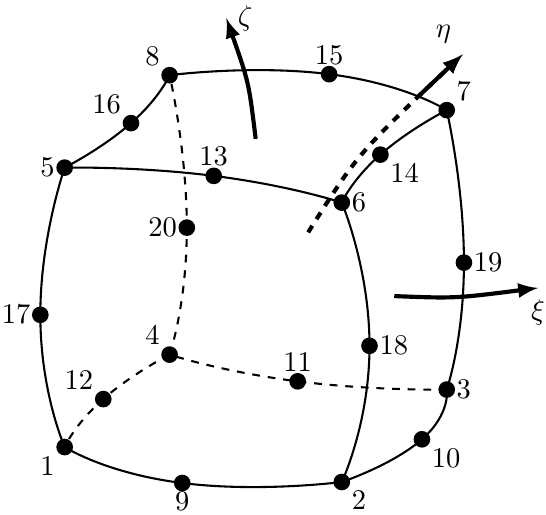
\includegraphics[scale=0.4]{Bilder/lsolid20_knoten}
\end{center}
\caption{Knotennummerierung des Lsolid20-Elements.}
\label{fig:lsolid20_knoten}
\end{figure}

Oberflächenkräfte werden durch Angabe der entsprechenden Elementseitenfläche definiert. Abbildung~\ref{fig:lsolid20_flaechen} zeigt die verwendete Nummerierung der Elementseitenflächen.

\begin{figure}[htb]
\centering
\begin{center}
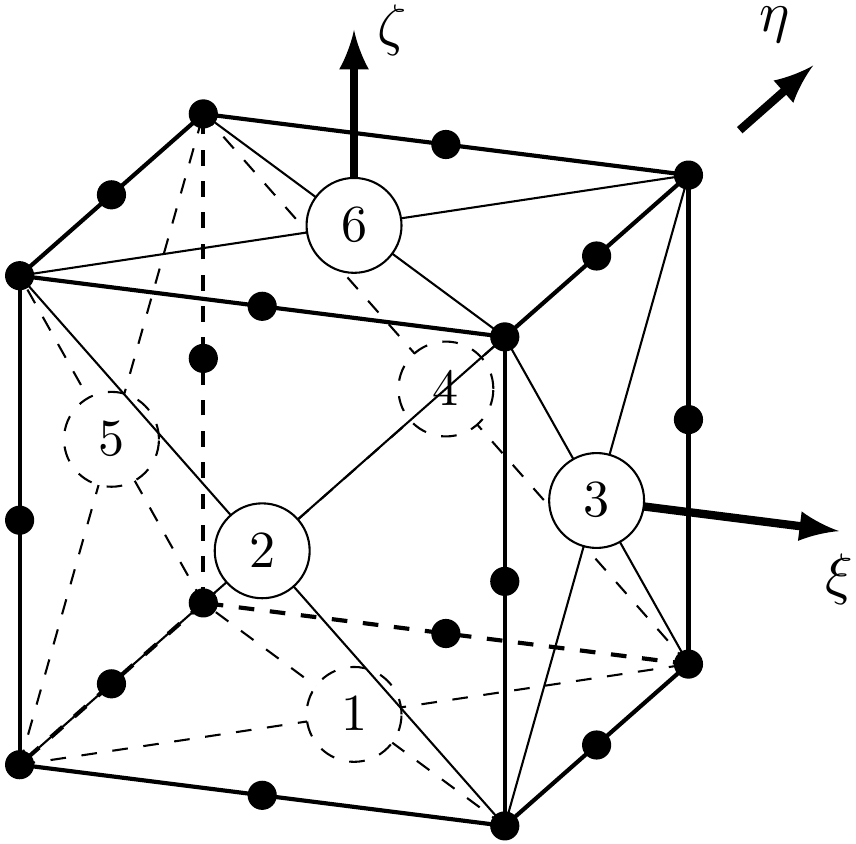
\includegraphics[scale=0.22]{Bilder/lsolid20_flaechen}
\end{center}
\caption{Flächennummerierung des Lsolid20-Elements.}
\label{fig:lsolid20_flaechen}
\end{figure}

\subsection{Steifigkeitsmatrix}

Die Elementsteifigkeitsmatrix $\mathbf{K}$ wird durch lagenweise Integration nach \cite{Panda1981} wie folgt berechnet:

\begin{equation}
\label{eq:layerwise_K}
\begin{split}
 \mathbf{K} = \: & \sum_{k=1}^{n_L} \int_{-1}^1 \int_{-1}^1 \int_{-1}^1 \mathbf{B}^\mathsf{T} \mathbf{C}_k \mathbf{B} \det \mathbf{J}  \cdot \frac{h_k}{t_L} \mathrm{d}\xi \mathrm{d}\eta \mathrm{d}\zeta_k \\
 & \text{mit } \mathbf{B} = \mathbf{B} \left( \xi, \eta, \zeta \right),\ \mathbf{J} = \mathbf{J} \left(\xi, \eta, \zeta \right) \ .
\end{split}
\end{equation}

Dabei bezeichnet $\mathbf{C}_k$ die Materialsteifigkeitsmatrix der $k$-ten Laminatlage, transformiert in das Bezugskoordinatensystem. Zur Berechnung der Verzerrungs-Verschiebungs-Matrix $\mathbf{B}$ und der \textsc{Jacobi}-Matrix $\mathbf{J}$ ist $\zeta_k$ durch die natürliche Elementkoordinate $\zeta$ zu substituieren:

\begin{equation}
\label{eq:zeta_k}
 \zeta = -1 + \frac{2 \sum_{i=1}^k \left(h_i \right) - h_k \left(1 - \zeta_k \right)}{t_L} \ ,
\end{equation}

wobei $h_i$ die Dicke der Laminatlage $i$ ist und $t_L = \sum_{i=1}^{n_L} h_i$ die Gesamtdicke des aus $n_L$ Einzellagen bestehenden Laminats bezeichnet.\par
Anzumerken ist, dass die Gesamtdicke $t_L$ des Laminats nicht notwendigerweise der tatsächlichen Elementdicke entsprechen muss. Bedingt durch die von $\zeta_k$ und dem einheitlichen Definitionsbereich von $\left\lbrace \left( \zeta, \zeta_k \right) \in \mathbb{R} | -1 \leq \left( \zeta, \zeta_k \right) \leq 1\right\rbrace$ der Dickenkoordinaten $\zeta$ und $\zeta_k$ über die Element- beziehungsweise Laminatlagendicke, wird der Lagenaufbau stets auf die tatsächliche Elementdicke skaliert. Bei der späteren Definition eines Laminats in dem FE-Programm sind demnach nur die Dickenverhältnisse $\nicefrac{h_k}{t_L}$ der Einzellagen entscheidend; die tatsächliche Lagendicke ist durch die Geometrie des FE-Modells vorgegeben.

\subsection{Geometrische Steifigkeitsmatrix}

Die Elementsteifigkeitsmatrix $\mathbf{K_g}$ wird durch lagenweise Integration nach \cite{Panda1981}, analog zur Steifigkeitsmatrix $\mathbf{K}$, wie folgt berechnet:

\begin{equation}
\label{eq:layerwise_Kg}
 \mathbf{K_g} = \sum_{k=1}^{n_L} \int_{-1}^1 \int_{-1}^1 \int_{-1}^1 \mathbf{G}^\mathsf{T} \mathbf{S}_k \mathbf{G} \det \mathbf{J}  \cdot \frac{h_k}{t_L} \mathrm{d}\xi \mathrm{d}\eta \mathrm{d}\zeta_k \ ,
\end{equation}

mit

{{\renewcommand{\arraystretch}{2.0}
\begin{equation}
\label{eq:lsolid20_G}
 \mathbf{G} = \begin{bmatrix}
    \dfrac{\partial N_1}{\partial x} & 0 & 0 & \dfrac{\partial N_2}{\partial x} & 0 & 0 & \cdots & \dfrac{\partial N_{20}}{\partial x} & 0 & 0 \\
    \dfrac{\partial N_1}{\partial y} & 0 & 0 & \dfrac{\partial N_2}{\partial y} & 0 & 0 & \cdots & \dfrac{\partial N_{20}}{\partial y} & 0 & 0 \\
    \dfrac{\partial N_1}{\partial z} & 0 & 0 & \dfrac{\partial N_2}{\partial z} & 0 & 0 & \cdots & \dfrac{\partial N_{20}}{\partial z} & 0 & 0 \\
    0 & \dfrac{\partial N_1}{\partial x} & 0 & 0 & \dfrac{\partial N_2}{\partial x} & 0 & \cdots & 0 & \dfrac{\partial N_{20}}{\partial x} & 0 \\
    0 & \dfrac{\partial N_1}{\partial y} & 0 & 0 & \dfrac{\partial N_2}{\partial y} & 0 & \cdots & 0 & \dfrac{\partial N_{20}}{\partial y} & 0 \\
    0 & \dfrac{\partial N_1}{\partial z} & 0 & 0 & \dfrac{\partial N_2}{\partial z} & 0 & \cdots & 0 & \dfrac{\partial N_{20}}{\partial z} & 0 \\
    0 & 0 & \dfrac{\partial N_1}{\partial x} & 0 & 0 & \dfrac{\partial N_2}{\partial x} & \cdots & 0 & 0 & \dfrac{\partial N_{20}}{\partial x} \\
    0 & 0 & \dfrac{\partial N_1}{\partial y} & 0 & 0 & \dfrac{\partial N_2}{\partial y} & \cdots & 0 & 0 & \dfrac{\partial N_{20}}{\partial y} \\
    0 & 0 & \dfrac{\partial N_1}{\partial z} & 0 & 0 & \dfrac{\partial N_2}{\partial z} & \cdots & 0 & 0 & \dfrac{\partial N_{20}}{\partial z}
 \end{bmatrix}
\end{equation}}

und

{{\renewcommand{\arraystretch}{2.0}
\begin{equation}
\label{eq:lsolid20_S}
 \mathbf{S} = \begin{bmatrix}
   \sigma_{x} & \tau_{xy} & \tau_{xz} & 0 & 0 & 0 & 0 & 0 & 0 \\
   \tau_{xy} & \sigma_{y} & \tau_{yz} & 0 & 0 & 0 & 0 & 0 & 0 \\
   \tau_{xz} & \tau_{yz} & \sigma_{z} & 0 & 0 & 0 & 0 & 0 & 0 \\
   0 & 0 & 0 & \sigma_{x} & \tau_{xy} & \tau_{xz} & 0 & 0 & 0 \\
   0 & 0 & 0 & \tau_{xy} & \sigma_{y} & \tau_{yz} & 0 & 0 & 0 \\
   0 & 0 & 0 & \tau_{xz} & \tau_{yz} & \sigma_{z} & 0 & 0 & 0 \\
   0 & 0 & 0 & 0 & 0 & 0 & \sigma_{x} & \tau_{xy} & \tau_{xz} \\
   0 & 0 & 0 & 0 & 0 & 0 & \tau_{xy} & \sigma_{y} & \tau_{yz} \\
   0 & 0 & 0 & 0 & 0 & 0 & \tau_{xz} & \tau_{yz} & \sigma_{z}
 \end{bmatrix} \ .
\end{equation}}

\subsection{Definition der Koordinatensysteme}

Die Gesamtsteifigkeitsmatrix $\mathbf{K}$, der Lastvektor $\mathbf{f}$ sowie der Vektor der diskreten Knotenkräfte $\mathbf{r}$ werden im globalen kartesischen Koordinatensystem $\left( x, y, z\right)$ aufgestellt. Weiterhin werden folgende Koordinatensysteme definiert:

\begin{itemize}
 \item Natürliches Koordinatensystem $\left( \xi, \eta, \zeta \right)$,
 \item Orthonormales Elementkoordinatensystem $\left( \bar{x}, \bar{y}, \bar{z} \right)$,
 \item Materialkoordinatensystem $\left(1, 2, 3\right)$,
 \item Lokales Knotenkoordinatensystem $\left(\hat{x}, \hat{y}, \hat{z}\right)$.
\end{itemize}

Die Koordinatensysteme sind entsprechend Abbildung~\ref{fig:lsolid20_koosy} definiert.

\begin{figure}[htb]
\centering
\begin{center}
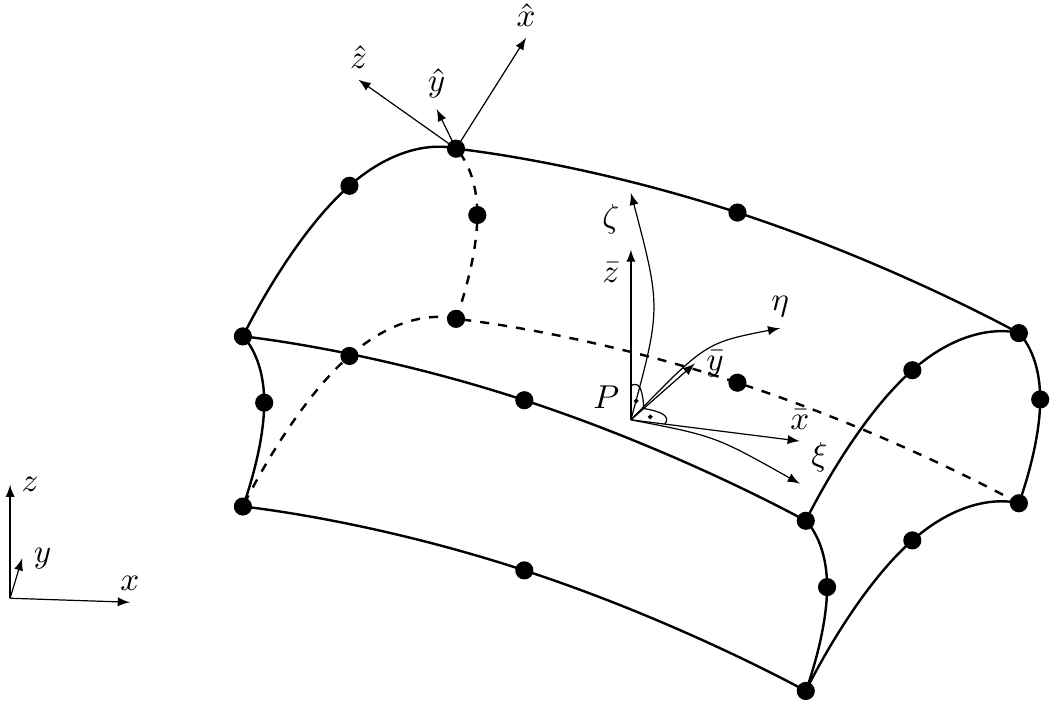
\includegraphics[scale=0.4]{Bilder/lsolid20_koosy}
\end{center}
\caption{Globales Koordinatensystem $\left( x, y, z \right)$, natürliches Koordinatensystem $\left( \xi, \eta, \zeta \right)$, orthonormales Elementkoordinatensystem $\left( \bar{x}, \bar{y}, \bar{z} \right)$ und lokales Knotenkoordinatensystem $\left(\hat{x}, \hat{y}, \hat{z}\right)$.}
\label{fig:lsolid20_koosy}
\end{figure}

Das natürliche Elementkoordinatensystem folgt als gekrümmtes Koordinatensystem der Elementkrümmung. Die $\xi$-$\eta$-Ebene mit $\zeta=0$ bildet somit stets die Mittenebene des Elements. \par
Das orthonormale Elementkoordinatensystem $\left( \bar{x}, \bar{y}, \bar{z} \right)$ ist lokal an dem jeweiligen Punkt $P$ innerhalb des Volumenelements definiert. Die $\bar{z}$-Achse des Elementkoordinatensystems folgt stets der Dickenrichtung $\zeta$ des Elements, die $\bar{x}$-Achse gibt die Fasernullrichtung $\varphi=0^\text{o}$ vor, sodass das Elementkoordinatensystem die Referenz für das relativ dazu rotierte Materialkoordinatensystem bildet. Im Allgemeinen ist die $\bar{x}$-Achse des Elementkoordinatensystems entlang der $\xi$-Koordinate des natürlichen Koordinatensystems ausgerichtet. Davon abweichend kann die Orientierung der $\bar{x}$-Achse durch einen benutzerdefinierten Vektor $\mathbf{v}$ vorgegeben werden. In diesem Fall ist die $\bar{x}$-Achse entlang der lokalen Projektion des Vektors $\mathbf{v}$ in die $\xi$-$\eta$-Mittenebene des Elements ausgerichtet. \par
An Knoten, an denen der Benutzer kein Knotenkoordinatensystem definiert, ist dieses automatisch entlang des globalen kartesischen Koordinatensystems ausgerichtet. Alternativ ist die Vorgabe des Knotenkoordinatensystems für jeden Knoten individuell durch den Nutzer möglich.

\subsection{Integrationsschema}

In den Lagenebenen erfolgt die Integration über eine reduzierte $2 \! \times \! 2$-\textsc{Gauss}-Integration, in Dickenrichtung wird die \textsc{Simpson}-Regel mit einem, drei, fünf, sieben oder neun Integrationspunkten je Laminatlage verwendet. Die Anzahl der Integrationspunkte je Lagendicke kann für jede Laminatlage separat definiert werden und die Werte 1, 2, 3, 5, 7 oder 9 annehmen. Die Gesamtanzahl der Integrationspunkte $n_{ges}$ je Finitem Element ist somit direkt proportional zur Anzahl der Laminatlagen $n_L$:

\begin{equation}
\label{eq:n_ip_ges}
  n_{ges} = 4 \cdot \sum_{k=1}^{n_L} n_{IP,k} \ .
\end{equation}

\newpage



\section{Benötigtes Vorgehen bei Hinzufügen eines neuen Elements}

\subsection{Eintragen in Globale Variablen}

Folgende Einträge sind in der Datei \emph{globale\_Variablen.f90} vorzunehmen:

\begin{itemize}
\item Eintragen des logischen Werts is\_\emph{Element}
\item Anlegen des Typs \emph{Element}\_type
\item Anlegen des Elements vom Typ \emph{Element}\_type
\end{itemize}

\subsection{Berücksichtigung im Einlesen der Kontrolldatei}

Folgende Einträge sind in der Datei \emph{input\_process\_line.f90} vorzunehmen:

\begin{itemize}
\item Einbau des Wortes des Elements in der Kontrolldatei
\end{itemize}

\subsection{Einbau des Einlesens des Elements}

Folgende Einträge sind in der Datei \emph{input\_tf.f90} vorzunehmen:

\begin{itemize}
\item Einbau des Einlesevorgangs entsprechend des angelegten Typs
\end{itemize}

\subsection{Berücksichtigung in Elementanzahl}

Folgende Einträge sind in der Datei \emph{init\_values.f90} vorzunehmen:

\begin{itemize}
\item Berücksichtigung der Anzahl des neuen Elements in der Größe \emph{num\_elements}
\end{itemize}

\subsection{Einbau in der statischen Lösung}

\begin{itemize}
\item Kontroll- bzw. Elementroutine in \emph{get\_stiffness\_matrices.f90} eintragen
\end{itemize}

\subsection{Einbau in der Beullösung}

\begin{itemize}
\item Kontroll- bzw. Elementroutine in \emph{get\_geometric\_stiffness\_matrix.f90} eintragen
\end{itemize}

\subsection{Einfügen des Object-Files in die Makefile-Datei}

Folgende Einträge sind in der Datei \emph{MakeFile} im Ordner \emph{/source} vorzunehmen:

\begin{itemize}
\item Hinzufügen der Object-Files der Routinen für das neue Element
\end{itemize}

\newpage

\chapter{Benutzerdefinierte Ergebnisausgabe über \emph{libuseroutput.so}}
\label{sec:libuseroutput}

Es besteht die Möglichkeit der Implementierung einer nutzerspezifischen Ergebnisausgabe in der benutzerdefinierten dynamischen Bibliothek \emph{libuseroutput.so}. Auf die Erstellung und Einbindung einer benutzerdefinierten dynamischen Bibliothek wird im Folgenden näher eingegangen.

Für die Erstellung der benutzerdefinierten Bibliothek werden die in Abbildung~\ref{fig:dirtree_libuseroutput} dargestellten Dateien und Ordner aus dem FiPPS\textsuperscript{2}-Repository benötigt.

\begin{figure}[htb]
\dirtree{%
.1 /.
.2 include.
.3 {*.mod}\DTcomment{Modul-Dateien der kompilierten FiPPS\textsuperscript{2}-Version}.
.3 {libmodule.a}\DTcomment{Bibliothek der FiPPS\textsuperscript{2}-Module}.
.2 source.
.3 {libfipps.a}\DTcomment{Bibliothek des FiPPS\textsuperscript{2}-Programms}.
.2 outputLibrary.
.3 Makefile.\DTcomment{Make-Datei für \emph{libuseroutput.so}}.
.3 {sol1\textunderscore output\textunderscore user.f90}\DTcomment{Benutzerdefinierte Ausgabe nach statischer Lösung}.
.3 {sol1\textunderscore output\textunderscore vtk.f90}\DTcomment{VTK-Ausgabe nach statischer Lösung}.
.3 {sol2\textunderscore output\textunderscore user.f90}\DTcomment{Benutzerdefinierte Ausgabe nach Stabilitätsanalyse}.
.3 {sol2\textunderscore output\textunderscore vtk.f90}\DTcomment{VTK-Ausgabe nach Stabilitätsanalyse}.
}
\caption{Verzeichnisstruktur der benötigten Dateien zur Erstellung einer dynamischen Bibliothek zur benutzerdefinierten Ergebnisausgabe.}
\label{fig:dirtree_libuseroutput}
\end{figure}

Der Ordner \emph{outputLibrary} beinhaltet die notwendigen Vorlagen der Subroutinen für die benutzerdefinierte Ergebnisausgabe und das entsprechende \emph{Makefile}. Hierbei ist zu beachten, dass die Subroutine \texttt{sol1\textunderscore output\textunderscore vtk()} bei Setzen des Keywords \emph{outputvtk} in \emph{control.fipps} (vergleiche Abschnitt~\ref{sec:einstellungsparameter}) zur Ausgabe der Ergebnisse der statischen Lösung als VTK"=Datei dient. Durch benutzerdefinierte Modifikation der Subroutine kann Einfluss auf die VTK"=Ausgabe genommen werden. Weiterhin dient die Subroutine als Muster für die Erstellung einer benutzerdefinierten Ergebnisausgabe.

Für die benutzerdefinierte Ergebnisausgabe steht die Subroutine \texttt{sol1\textunderscore output\textunderscore user()} zur Verfügung. Diese wird bei Setzen des Keywords \emph{outputuser} in \emph{control.fipps} (vergleiche Abschnitt~\ref{sec:einstellungsparameter}) nach der statischen Lösung aufgerufen. Hierbei ist zu beachten, dass sich die Argumente der Subroutine von \texttt{sol1\textunderscore output\textunderscore vtk()} unterscheiden. Neben den Basisdaten zum FE-Modell \texttt{fesim}, dem Verschiebungsvektor \texttt{Utot} und der Nummer des aktuellen Subcase \texttt{scloop} stehen folgende Argumente zur Verfügung:

\begin{itemize}
  \item \texttt{Fout}: Vollständig besetzter Kraftvektor mit allen externen Lasten,
  \item \texttt{cdi}: Beiwert des induzierten Widerstands aus einer gegebenenfalls definierten dreidimensionalen Fluid-Strukturkopplung mittels APAME (vergleiche Abschnitt~\ref{sec:fluid-strukturkopplung}),
  \item \texttt{aeroConverged}: Boolean-Flag über die Konvergenz einer gegebenenfalls definierten zwei- oder dreidimensionalen Fluid-Strukturkopplung im aktuellen Subcase \texttt{scloop} (vergleiche Abschnitt~\ref{sec:fluid-strukturkopplung}; \texttt{.True.}: konvergiert, \texttt{.False.}: nicht konvergiert).
\end{itemize}

Es ist zu beachten, dass die Nutzung der benutzerdefinierten Ausgabe \texttt{sol1\textunderscore output\textunderscore user()} durch Setzen des Keywords \emph{outputuser} zu einem geringfügig erhöhten Speicherbedarf von FiPPS\textsuperscript{2} führen kann, da der vollständig besetzte Lastvektor über das Lösen des Gleichungssystems für die statische Lösung behalten wird.

Analog zu den Subroutinen \texttt{sol1\textunderscore output\textunderscore vtk()}  und \texttt{sol1\textunderscore output\textunderscore user()} zur Ausgabe der Ergebnisse der statischen Strukturlösung dienen die Subroutinen \texttt{sol2\textunderscore output\textunderscore vtk()} und \texttt{sol2\textunderscore output\textunderscore user()} zur Ausgabe der Lösungen der linearen Stabilitätsanalyse. Der Aufruf der Subroutinen ist ebenfalls an das jeweilige Keyword \emph{outputvtk} und \emph{outputuser} in \emph{control.fipps} gebunden.

Nach Kompilieren der benutzerdefinierten Bibliothek ist der Pfad zu der erzeugten dynamischen Bibliothek \emph{libuseroutput.so} der Umgebungsvariablen \texttt{LD\textunderscore LIBRARY\textunderscore PATH} hinzuzufügen. Liegt die kompilierte dynamische Bibliothek exemplarisch im Verzeichnis

\begin{center}
\texttt{/home/user/outputLibrary/libuseroutput.so}
\end{center}

kann die Ergänzung der Umgebungsvariablen durch folgenden Befehl vorgenommen werden:

\begin{center}
\texttt{export LD\textunderscore LIBRARY\textunderscore PATH=/home/user/outputLibrary:\$LD\textunderscore LIBRARY\textunderscore PATH}
\end{center}

wodurch der Pfad zu den bereits definierten Suchpfaden dynamischer Bibliotheken hinzugefügt wird. Durch obigen Befehl wird der Pfad als erster Suchpfad in \texttt{LD\textunderscore LIBRARY\textunderscore PATH} gesetzt, sodass die benutzerdefinierte Bibliothek anstelle der Standardbibliothek in FiPPS\textsuperscript{2} genutzt wird.

\newpage

\chapter{Debugging-Optionen}

\section{Ausgabe von Werten}

\subsection{Herausschreiben einer quadratischen Matrix}

Über die Subroutine \emph{write\_quad\_Matrix}

\subsection{Grafische Ausgabe der Gesamtsteifigkeitsmatrix}

mit PETSc über die Option -draw\_pause <pause>, wobei <pause> die länge der Pause in Sekunden darstellt. Um die Matrix bis zum manuellen schließen des Fensters anzuzeigen kann der Wert <pause>=-1 genutzt werden.

\section{Vergleich mit ANSYS}

\subsection{Herausschreiben der Elementsteifigkeitsmatrizen}

Mit dem undokumentierten Befehl /DEBUG können für alle Elemente die Steifigkeitsmatrizen (und auch geometrischen Steifigkeitmatrizen) ausgegeben werden.

% \begin{center}
\lstset{language=TeX}
\begin{lstlisting}[columns=fullflexible,basicstyle=\ttfamily,caption=Eingabe zur Ausgabe der Elementsteifigkeitsmatrix in ANSYS,captionpos=b]
/solu
/debug,3,1,1,1,1,1
/output,filename,out	(where filename is any name you desire;
			out is the file extension)
solve 
/output,term
\end{lstlisting}
% \end{center}

gefunden unter: \url{http://www.cadfem.de/fileadmin/files/9_service_newsletter/2003/0308/Newsletter_08_2003.pdf}

\subsection{Herausschreiben des Lastvektors}

Der Lastvektor einer statischen Lösung lässt sich über den Umweg einer Substructure-Analyse erlangen. Die nötigen Eingaben lauten:

% \begin{center}
\lstset{language=TeX}
\begin{lstlisting}[columns=fullflexible,basicstyle=\ttfamily,caption=Eingabe zur Ausgabe des Lastvektors in ANSYS,captionpos=b]
/solu
antype,substr
seopt,file,1,1
m,all,all
/output,filename,out	(where filename is any name you desire;
			out is the file extension)
solve
/output
\end{lstlisting}
% \end{center}

gefunden unter: \url{http://www.scribd.com/doc/8120884/ANSYS-Stiffness-Matrix-v8p1}.

\newpage

\chapter{Input-Karten}

\section{Einleitung}

Sämtliche Input-Karten sind dem Löser als einzelne Dateien zur Verfügung zu stellen. Welche Dateien im Modell berücksichtigt werden, muss in einer Datei mit dem Namen \emph{control.fipps} spezifiziert werden. In dieser wird zusätzlich die gewünschte Lösungsart angegeben. Über den Parameter \emph{sol} kann eine ausschließlich statische Lösung (\emph{sol=1}) oder eine linearisierte Beulanalyse (\emph{sol=2}) gewählt werden. Wird die Beulanalyse gewählt, ist zusätzlich die Anzahl der gesuchten kleinsten Eigenwerte über den Parameter \emph{numEigVal} anzugeben. Die Reihenfolge der Angabe in der Datei \emph{control.fipps} ist egal. Lediglich in der ersten Zeile muss als I10-Wert die Anzahl der Zeilen in der Kontrolldatei angegeben werden.

In der \emph{control.fipps} wird zudem die Ausgabe gesteuert.

\lstset{language=Fortran}
\begin{lstlisting}[caption=Beispiel einer \emph{control.fipps}-Datei,captionpos=b]
       24
coord
load
force
beam2
quad8
mat1
mat8
lam8
pbeam
pcomp
spcadd
spc1
subcase
node
coupling
temperature
failure
sol=2
numEigVal=4
shellResPos=1
outputvtk
outputshort
outputelemcoord
outputboundcond
\end{lstlisting}

Jede Inputdatei ist in dem Format vorzugeben, dass die einzelnen Karten vorgeben. In der ersten Zeile einer jeden Datei muss die Anzahl der zu berücksichtigenden Einträge (also Zeilen) stehen. Die erste Zeile, in der die Zeilenanzahl steht, wird hierbei nicht berücksichtigt.

\subsection{Beschreibung der Dateieinträge}

\begin{tabularx}{\textwidth}{llX}
\toprule
Eintrag			& Dateiname			& Inhalt	\\
\midrule
aeroload2d		& aeroload2ds.fipps		& Definition einer zweidimensionalen aerodynamischen Last, berechnet über die integrierte Fluid-Struktur-Kopplung	\\
aeroload3d		& aeroload3ds.fipps		& Definition einer dreidimensionalen aerodynamischen Last, berechnet über die integrierte Fluid-Struktur-Kopplung	\\
beam2			& beam2.fipps			& Definition von 2"=Konten"=Balkenelemente	\\
beam2temp		& beam2temps.fipps		& Definition von thermomechanischen Lasten auf Beam2"=Elemente \\
contact\_node\_beam2	& contact\_node\_beam2.fipps	& Knoten"=Beam2"=Element"=Kontaktdefinition	\\
contact\_node\_quad8	& contact\_node\_quad8.fipps	& Knoten"=Quad8"=Element"=Kontaktdefinition	\\
contact\_node\_lsolid20	& contact\_node\_lsolid20.fipps	& Knoten"=Lsolid20"=Element"=Kontaktdefinition	\\
coord			& coord.fipps			& Defintion von Koordinatensystemen	\\
coupling		& couplings.fipps		& Defintion der Kopplung von Freiheiten	\\
force			& forces.fipps			& Defintion von Kräften	\\
lam8			& lam8.fipps			& Definition von Laminaten	\\
lam20			& lam20.fipps			& Definition von Laminaten für das Lsolid20"=Ele"-ment	\\
load			& loads.fipps			& Definition einer Last aus Kräften und Momenten \\
lsolid20 		& lsolid20.fipps		& Definition des 20-Knoten Layered Solid-Elements Lsolid20	\\
lsolid20temp		& lsolid20temps.fipps		& Definition von thermomechanischen Lasten auf Lsolid20"=Ele"-mente \\
failure			& failure.fipps			& Definition von Festigkeits- / Versagenskriterien	\\
mat1			& mat1.fipps			& Definition von isotropen Materialien	\\
mat8			& mat8.fipps			& Definition von orthotropen Materialien	\\
mat20			& mat20.fipps			& Definition von orthotropen Materialien nach dem dreidimensionalen Elastizitätsgesetz	\\
moment			& moments.fipps			& Definition von Momenten	\\
mpc			& mpc.fipps			& Definition von Multi Point Constraints	\\
\bottomrule
\end{tabularx}

\newpage

\begin{tabularx}{\textwidth}{llX}
\toprule
Eintrag			& Dateiname			& Inhalt	\\
\midrule
mpcadd			& mpcadd.fipps			& Definition von Multi Point Constraint Sets	\\
multistep		& multistep.fipps		& Definition einer mehrschrittigen FE-Analyse  \\
node			& nodes.fipps			& Definition von Knoten	\\
p2load			& p2loads.fipps			& Definition von Linienlasten auf Beam2"=Elemente	\\
p3load			& p3loads.fipps			& Definition von Drucklasten auf Tria3"=Elemente	\\
p8load			& p8loads.fipps			& Definition von Drucklasten auf Quad8"=Elemente	\\
p20load			& p20loads.fipps		& Definition von Oberflächenkräften auf Lsolid20"=Ele"-mente	\\
pbeam			& pbeam.fipps			& Definition von Balkenelementeigenschaften	\\
pcomp			& pcomp.fipps			& Definition von Schalenelementeigenschaften (geschichteter Aufbau)	\\
plsolid			& plsolid.fipps			& Definition von Eigenschaften des Lsolid20"=Ele"-ments	\\
pshell			& pshell.fipps			& Definition von Schalenelementeigenschaften (isotrop, ungeschichtet)	\\
quad4			& quad4.fipps			& Definition von 4"=Knoten"=Schalenelementen	\\
quad8			& quad8.fipps			& Definition von 8"=Knoten"=Schalenelementen	\\
quad8temp		& quad8temps.fipps		& Definition von thermomechanischen Lasten auf Quad8"=Ele"-mente \\
spc1			& spc1.fipps			& Definition von gesperrten Freiheiten	\\
spcadd			& spcadd.fipps			& Definition von Set gesperrter Freiheiten	\\
subcase			& subcase.fipps			& Lastfalldefinition	\\
temperature		& temperatures.fipps		& Definition von thermomechanischen Lasten auf Knoten \\
tria3			& tria3.fipps			& Definition von 3"=Knoten"=Dreiseckelementen	\\
\bottomrule
\end{tabularx}


\subsection{Beschreibung der Einstellungsparameter}
\label{sec:einstellungsparameter}

\begin{tabularx}{\textwidth}{lX}
\toprule
Eintrag		& Inhalt	\\
\midrule
sol		& Einstellung der gewünschten Lösungsart \newline 1 - statische Rechnung \newline 2 - Beulrechnung (mit vorheriger statischer Rechnung)\\
numEigVal	& Anzahl der gewünschten Eigenwerte im Falle einer Beulrechnung (sol = 2). Es handelt sich dabei um die Mindestenanzahl an Eigenwerten, die das Konvergenzkriterium erfüllen müssen. \\
blocksize	& Dieser Parameter ist für eine verbesserte Abschätzung der Nichtnullelement in den Steifigkeitsmatrizen notwendig. Dabei werden jeweils ``blocksize''-Werte einer Matrixzeile zusammengefasst und für dieser die Anzahl der Nichtnullelemente statt für die Elemente der gesamten Zeile bestimmt. Sinnvolle Werte liegen bei 500  bis 1000. Bei zu kleinen Werten kehrt sich der Effekt um, da dann für die Abschätzung schon zuviel Speicher benötigt wird. Im Falle von blocksize = 1 wird zur Abschätzung Speicher in der Größenordnung der Größe der Steifigkeitsmatrizen als dense verwendet. Dafür erhält man die beste Abschätzung. \newline Dieser Parameter muss nicht vorhanden werden. Wenn eine Vielzahl vom MPCs oder Kontakten im Modell vorhanden sind, sollte dieser Wert aber gesetzt werden.\\
shellResPos     & Schalter, an welcher Stelle die Dehnungen von Schalenelementen berechnet und ausgegeben werden sollen (0 - MID, 1 - TOP, 2 - BOT). Der Standardwert ist 0. \\
outputuser      & Es werden die  Ausgaberoutinen \texttt{sol1\textunderscore user\textunderscore output()} und \texttt{sol2\textunderscore user\textunderscore output()} aus der benutzerdefinierten dynamischen Bibliothek \emph{libuseroutput.so} aufgerufen (siehe Kapitel~\ref{sec:libuseroutput}). \\
outputvtk       & Die Ergebnisse werden als VTK-Dateien ausgegeben. \\
outputshort     & Es wird eine output\_FEM.txt Datei herausgeschrieben, in der pro Lastfall die wichtigsten Informationen stehen. \\
outputelemcoord & Es werden die Elementkoordinatensystem in die VTK-Datei ausgeben. Diese Option wird nur berücksichtigt, wenn outputvtk aktiv ist. \\
outputboundcond & Es werden die Randbedingungen in die VTK-Datei ausgeben. Diese Option wird nur berücksichtigt, wenn outputvtk aktiv ist. \\
aeroDisplEps    & Dieser Parameter definiert das Abbruchkriterium für die Fluid"-Strukturkopplung. Bei relativen Verschiebungsänderungen kleiner als dieser Wert, bricht die Iteration ab. \\
calculatetse	& Es erfolgt die Berechnung der Gesamtdehnungsenergie (Total Strain Energy - TSE). \\
calculateelementaltse   & Es erfolgt die Berechnung der elementweisen Gesamtdehnungsenergie (Total Strain Energy - TSE). \\
\bottomrule
\end{tabularx}

\newpage

\section{Knoten}

\subsection{Nodes}

\subsubsection{Beschreibung}

Die Karte definiert die Knoten.

\subsubsection{Input-Karte}

Alle Karten müssen zeilenweise ausgefüllt werden.\\
Die Datei muss den Namen \emph{nodes.fipps} haben.

\begin{table}[htbp]
\centering
\begin{tabularx}{\textwidth}{cCCCCCCCC}
\toprule
Karte 1	& 1		& 2		& 3		& 4		& 5		& 6		& 7	& 8	\\
\midrule
Variable& cid		& coord1	& coord2	& coord3	& - 		& -	  	& -	& -	\\
Typ	& I>0		& R		& R		& R  		& -		& -	  	& -	& -	\\
Standard& -		& -		& -		& -		& -		& -		& -	& -	\\
Hinweis	& 1		& -		& -		& -		& -		& -		& -	& -	\\
aktuell	& \multirow{2}{*}{\checkmark}	& \multirow{2}{*}{\checkmark}	& \multirow{2}{*}{\checkmark}	& \multirow{2}{*}{\checkmark}	& \multirow{2}{*}{-}	& \multirow{2}{*}{-}	& \multirow{2}{*}{-}	& \multirow{2}{*}{-}	\\
genutzt \\
\bottomrule
\end{tabularx}
% \caption{FiPPS Input-Karte für Knoten \label{Tab_Inp_nodes}}
\end{table}

\subsubsection{Beschreibung}

\begin{tabularx}{\textwidth}{cXcc}
\toprule
Variable	& Beschreibung																						& Typ		& Format\\
\midrule
cid		& Koordinatensystem-ID	(siehe Hinweis 1)	& Integer > 0	& I10	\\
coordi 		& Koordinaten der Knoten (x,y,z)		& Real		& 3E24.16\\
\bottomrule
\end{tabularx}

\subsubsection{Hinweise}

\begin{enumerate}
\item Knoten können in beliebigen Koordinatensystemen definiert sein. Zur Zeit stehen nur kartesische Rechtssysteme zur Verfügung.
\end{enumerate}

\newpage

\section{Elemente}

\subsection{Beam2}

\subsubsection{Beschreibung}

Die Karte definiert ein 2-Knoten-Balkenelement mit linearem Verschiebungsansatz. Das Element kann Zug/Druck, Biegung und Torsion übertragen. Es ist definiert nach \cite{Prze1968}.\\
Die Datei muss den Namen \emph{beam2.fipps} haben.

\subsubsection{Input-Karte}

Alle Karten müssen zeilenweise ausgefüllt werden

\begin{table}[htbp]
\centering
\begin{tabularx}{\textwidth}{cCCCCCCCC}
\toprule
Karte 1	& 1		& 2		& 3		& 4		& 5		& 6		& 7	& 8	\\
\midrule
Variable& pid		& nid1		& nid2		& x1  		& x2 		& x3 	 	& n0	& -	\\
Typ	& I>0		& I>0		& I>0		& R  		& R		& R  		& I>0	& -	\\
Standard& -		& -		& -		& -		& -		& -		& -	& -	\\
Hinweis	& -		& -		& -		& 1		& 1		& 1		& 2	& -	\\
aktuell	& \multirow{2}{*}{\checkmark}	& \multirow{2}{*}{\checkmark}	& \multirow{2}{*}{\checkmark}	& \multirow{2}{*}{\checkmark}	& \multirow{2}{*}{\checkmark}	& \multirow{2}{*}{\checkmark}	& \multirow{2}{*}{-}	& \multirow{2}{*}{-}	\\
genutzt \\
\bottomrule
\end{tabularx}
% \caption{FiPPS Input-Karte für Beam2-Element \label{Tab_Inp_Beam2}}
\end{table}

\subsubsection{Beschreibung}

\begin{tabularx}{\textwidth}{cXcc}
\toprule
Variable& Beschreibung					& Typ			& Format\\
\midrule
pid		& Property-ID				& Integer > 0	& I10	\\
nidi		& Knoten-ID				& Integer > 0	& 2I10	\\
xi   		& Komponenten des Orientierungsvektors des Balkenhauptachsenkoordinatensystems am Knoten 1 in lokalen Koordinaten. Der Vektor muss nicht normiert sein. (siehe Hinweis 1)	& Real			& 3E23.16\\
n0		& Knoten für Orientierungsvektor des Balkenhauptachsenkoordinatensystems am Knoten 1 (siehe Hinweis 2)					& Integer > 0	& I10	\\
\bottomrule
\end{tabularx}

\subsubsection{Hinweise}

\begin{enumerate}
\item Wird kein Wert oder 0.0 für x1, x2, x3 angegeben, wird das lokale Koordinatensystem nach dem Prinzip des Beam4 aus Ansys bestimmt. 
\item In der aktuellen Version nicht implementiert, intern gelöst
\end{enumerate}

\newpage

\subsection{Tria3}

Dieses Element wird derzeit nicht unterstützt.

\subsubsection{Beschreibung}

Dieses Element ist in die aktuellen Version nicht mehr funktionsfähig. Bei Bedarf bitte an die Entwickler wenden.

Die Karte definiert ein 3-Knoten-Dreieckselement mit linearem Verschiebungsansatz.\\
Die Datei muss den Namen \emph{tria3.fipps} haben.

\subsubsection{Input-Karte}

\begin{table}[htbp]
\centering
\begin{tabularx}{\textwidth}{cCCCCCCCC}
\toprule
Karte 1	& 1		& 2		& 3		& 4		& 5		& 6		& 7		& 8	\\
\midrule
Variable& pid		& nid1		& nid2		& nid3		& theta		& atype		& offset	& -	\\
Typ	& I>0		& I>0		& I>0		& I>0		& R		& C		& R		& -	\\
Standard& -		& -		& -		& -		& -		& -		& -		& -	\\
Hinweis	& -		& -		& -		& -		& 1		& 2		& 2		& -	\\
aktuell	& \multirow{2}{*}{\checkmark}	& \multirow{2}{*}{\checkmark}	& \multirow{2}{*}{\checkmark}	& \multirow{2}{*}{\checkmark}	& \multirow{2}{*}{\checkmark}	& \multirow{2}{*}{-}	& \multirow{2}{*}{-}	& \multirow{2}{*}{-}	\\
genutzt \\
\bottomrule
\end{tabularx}
% \caption{FiPPS Input-Karte für Tria3-Element \label{Tab_Inp_Tria3}}
\end{table}

\subsubsection{Beschreibung}

\begin{tabularx}{\textwidth}{cXcc}
\toprule
Variable& Beschreibung									& Typ		& Format\\
\midrule
pid	& Property-ID									& Integer > 0	& I10	\\
nidi	& Knoten-ID									& Integer > 0	& 3I10	\\
theta	& Angle between element and material coordinate System (siehe Hinweis 1)	& Real		& E23.16\\
atype	& Angle type, 'deg' or 'rad'							& Character	& A3	\\
offset	& material coordinate offset from FE reference plane (thickness direction)	& Real		& E23.16\\
\bottomrule
\end{tabularx}

\subsubsection{Hinweise}

\begin{enumerate}
\item Der Winkel zwischen Material und Elementkoordinatensystem ...
\item Diese größen werden in aktuellen FiPPS-Version automatisch auf 'rad' bzw. 0.0 gesetzt.
\end{enumerate}

\newpage

\subsection{Quad8}

\subsubsection{Beschreibung}

Die Karte definiert ein 8-Knoten-Viereckselement mit biquadratischem Verschiebungsansatz (Serendipity-Typ). Das Element kann doppeltgekrümmt sein.\\
Die Datei muss den Namen \emph{quad8.fipps} haben.

\subsubsection{Input-Karte}

Alle Karten müssen zeilenweise ausgefüllt werden

\begin{table}[htbp]
\centering
\begin{tabularx}{\textwidth}{cCCCCCCCC}
\toprule
Karte 1	& 1		& 2		& 3		& 4		& 5		& 6		& 7	& 8		\\
\midrule
Variable& pid		& nid1		& nid2		& nid3		& nid4		& nid5		& nid6	& nid7		\\
Typ	& I>0		& I>0		& I>0		& I>0		& I>0		& I>0		& I>0	& I>0		\\
Standard& -		& -		& -		& -		& -		& -		& -	& -		\\
Hinweis	& -		& -		& -		& -		& -		& -		& -	& -		\\
aktuell	& \multirow{2}{*}{\checkmark}	& \multirow{2}{*}{\checkmark}	& \multirow{2}{*}{\checkmark}	& \multirow{2}{*}{\checkmark}	& \multirow{2}{*}{\checkmark}	& \multirow{2}{*}{\checkmark}	& \multirow{2}{*}{\checkmark}	& \multirow{2}{*}{\checkmark}	\\
genutzt \\
\\
Karte 2	& 9		& 10		& 11		& 12		& 13		& 14		& 15	& 16	\\
\midrule
Variable& nid8		& theta		& atype		& offset	& -		& -		& -	& -	\\
Typ	& I>0		& R		& C		& R		& -		& -		& -	& -	\\
Standard& -		& -		& -		& -		& -		& -		& -	& -	\\
Hinweis	& -		& 1		& -		& -		& -		& -		& -	& -	\\
aktuell	& \multirow{2}{*}{\checkmark}	& \multirow{2}{*}{\checkmark}	& \multirow{2}{*}{\checkmark}	& \multirow{2}{*}{\checkmark}	& \multirow{2}{*}{-}	& \multirow{2}{*}{-}	& \multirow{2}{*}{-}	& \multirow{2}{*}{-}	\\
genutzt \\
\bottomrule
\end{tabularx}
% \caption{FiPPS Input-Karten für Quad8-Element \label{Tab_Inp_Quad8}}
\end{table}

\subsubsection{Beschreibung}

\begin{tabularx}{\textwidth}{cXcc}
\toprule
Variable& Beschreibung									& Typ		& Format\\
\midrule
pid	& Property-ID									& Integer > 0	& I10	\\
nidi	& Knoten-ID									& Integer > 0	& 8I10	\\
theta	& Angle between element and material coordinate System (siehe Hinweis 1)	& Real		& E23.16\\
atype	& Angle type, 'deg' or 'rad'							& Character	& 3A	\\
offset	& material coordinate offset from FE reference plane (thickness direction)	& Real		& E23.16\\
\bottomrule
\end{tabularx}

\subsubsection{Hinweise}

\begin{enumerate}
\item Der Winkel zwischen Material und Elementkoordinatensystem ...
\end{enumerate}

\newpage

\subsection{Lsolid20}
%
\subsubsection{Beschreibung}
%
Die Eingabekarte definiert ein Lsolid20-Element. Das Element ist als Layered Solid-Element mit 20 Knoten ausgeführt. Der Laminataufbau kann aus einer beliebigen Anzahl orthotroper Einzellagen bestehen. Abbildung~\ref{fig:lsolid20_knoten} stellt die verwendete Knotennummerierung dar.\\
Die Datei muss den Namen \emph{lsolid20.fipps} haben.
%
\subsubsection{Input-Karte}
%
\begin{table}[htbp]
\centering
\begin{tabularx}{\textwidth}{cCCCCCCCC}
\toprule
Karte 1         & 1     & 2     & 3     & 4     & 5     & 6     & 7     & 8       \\
\midrule
Variable        & pid   & nid1  & nid2  & nid3  & nid4  & nid5  & nid6  & nid7    \\
Typ             & I>0   & I>0   & I>0   & I>0   & I>0   & I>0   & I>0   & I>0     \\
Standard        & -     & -     & -     & -     & -     & -     & -     & -       \\
Hinweis         & -     & -     & -     & -     & -     & -     & -     & -       \\
aktuell         & \multirow{2}{*}{\checkmark} & \multirow{2}{*}{\checkmark} & \multirow{2}{*}{\checkmark} & \multirow{2}{*}{\checkmark} & \multirow{2}{*}{\checkmark} & \multirow{2}{*}{\checkmark} & \multirow{2}{*}{\checkmark} & \multirow{2}{*}{\checkmark}  \\
genutzt \\
\\
Karte 2         & 9     & 10    & 11    & 12    & 13    & 14    & 15    & 16      \\
\midrule
Variable        & nid8  & nid9  & nid10 & nid11 & nid12 & nid13 & nid14 & nid15   \\
Typ             & I>0   & I>0   & I>0   & I>0   & I>0   & I>0   & I>0   & I>0     \\
Standard        & -     & -     & -     & -     & -     & -     & -     & -       \\
Hinweis         & -     & -     & -     & -     & -     & -     & -     & -       \\
aktuell         & \multirow{2}{*}{\checkmark} & \multirow{2}{*}{\checkmark} & \multirow{2}{*}{\checkmark} & \multirow{2}{*}{\checkmark} & \multirow{2}{*}{\checkmark} & \multirow{2}{*}{\checkmark} & \multirow{2}{*}{\checkmark} & \multirow{2}{*}{\checkmark}  \\
genutzt \\
\\
Karte 3         & 17    & 18    & 19    & 20    & 21    & 22    & 23    & 24      \\
\midrule
Variable        & nid16 & nid17 & nid18 & nid19 & nid20 & -  & -  & -   \\
Typ             & I>0   & I>0   & I>0   & I>0   & I>0   & -  & -  & -   \\
Standard        & -     & -     & -     & -     & -     & -  & -  & -   \\
Hinweis         & -     & -     & -     & -     & -     & -  & -  & -   \\
aktuell         & \multirow{2}{*}{\checkmark} & \multirow{2}{*}{\checkmark} & \multirow{2}{*}{\checkmark} & \multirow{2}{*}{\checkmark} & \multirow{2}{*}{\checkmark} & \multirow{2}{*}{-}  & \multirow{2}{*}{-}  & \multirow{2}{*}{-}   \\
genutzt \\
\bottomrule
\end{tabularx}
\end{table}

\subsubsection{Beschreibung}

\begin{tabularx}{\textwidth}{cXcc}
\toprule
Variable  & Beschreibung  & Typ          & Format  \\
\midrule
pid       & Property-ID   & Integer > 0  & I10     \\
nidi      & Knoten-ID     & Integer > 0  & 20I10   \\
\bottomrule
\end{tabularx}

\newpage

\section{Belastungen}

\subsection{Load}

\subsubsection{Beschreibung}

Diese Karte definiert ein Lastenset aus Einzellasten. Diese können einzeln skaliert werden.\\
Die Datei muss den Namen \emph{loads.fipps} haben. Diese Karte muss erstellt werden, sobald das Modell belastet werden soll.

\subsubsection{Input-Karte}

\begin{table}[htbp]
\centering
\begin{tabularx}{\textwidth}{cCCCCCCCC}
\toprule
Karte 1	& 1		& 2		& 3		& 4		& 5		& 6		& 7		& 8		\\
\midrule
Variable& lcid		& sfaci		& lidi		& -		& -		& -		& -		& -		\\
Typ	& I>0		& R		& I>0		& -		& -		& -		& -		& -		\\
Standard& -		& -		& -		& -		& -		& -		& -		& -		\\
Hinweis	& 1		& -		& -		& -		& -		& -		& -		& -		\\
aktuell	& \multirow{2}{*}{\checkmark}	& \multirow{2}{*}{\checkmark}	& \multirow{2}{*}{\checkmark}	& \multirow{2}{*}{-}	& \multirow{2}{*}{-}	& \multirow{2}{*}{-}	& \multirow{2}{*}{-}	& \multirow{2}{*}{-}	\\
genutzt \\
\bottomrule
\end{tabularx}
% \caption{FiPPS Input-Karte für ein Lastenset \label{Tab_Inp_Loads}}
\end{table}

\subsubsection{Beschreibung}

\begin{tabularx}{\textwidth}{cXcc}
\toprule
Variable& Beschreibung					& Typ		& Format\\
\midrule
lcid	& LoadCase-ID					& Integer > 0	& I10	\\
sfaci	& Skalierungsfaktor für die  Einzellast		& Real		& E23.16\\
lidi	& Load-ID der Einzellast			& Integer > 0	& I10	\\
\bottomrule
\end{tabularx}

\subsubsection{Hinweise}

\begin{enumerate}
\item Mehrere Einzellasten können zu einem Set zusammengefasst werden, indem sie die gleiche LoadCaseID (lcid) erhalten.
\item Der Faktor sfac muss für alle Einzellasten eines Lastensets (jede Zeile) identisch sein. Er kann in der aktuellen Version nicht gesetzt werden, sondern hat automatisch den Wert eins.
\end{enumerate}

\newpage

\subsection{Force}

\subsubsection{Beschreibung}

Diese Karte definiert eine diskrete Einzelkraft auf einen Knoten.\\
Die Datei muss den Namen \emph{forces.fipps} haben.

\subsubsection{Input-Karte}

\begin{table}[htbp]
\centering
\begin{tabularx}{\textwidth}{cCCCCCCCC}
\toprule
Karte 1	& 1		& 2		& 3		& 4		& 5		& 6		& 7	& 8	\\
\midrule
Variable& lid		& nid		& fac		& n1		& n2		& n3		& -	& -	\\
Typ	& I>0		& I>0		& R		& R		& R		& R		& -	& -	\\
Standard& -		& -		& -		& -		& -		& -		& -	& -	\\
Hinweis	& -		& -		& -		& 2		& 2		& 2		& -	& -	\\
aktuell	& \multirow{2}{*}{\checkmark}	& \multirow{2}{*}{\checkmark}	& \multirow{2}{*}{\checkmark}	& \multirow{2}{*}{\checkmark}	& \multirow{2}{*}{\checkmark}	& \multirow{2}{*}{\checkmark}	& \multirow{2}{*}{-}	& \multirow{2}{*}{-}	\\
genutzt \\
\bottomrule
\end{tabularx}
% \caption{FiPPS Input-Karte für eine Kraft \label{Tab_Inp_Force}}
\end{table}

\subsubsection{Beschreibung}

\begin{tabularx}{\textwidth}{cXcc}
\toprule
Variable& Beschreibung																& Typ		& Format\\
\midrule
lid		& Load-ID															& Integer > 0	& I10	\\
nid		& Node-ID des Knotens an dem die Kraft wirkt											& Integer > 0	& I10	\\
fac		& Skalierungsfaktor														& Real		& E23.16\\
ni		& Komponenten des Vektors der Kraft (Translationen), gemessen in dem Koordinatensystem, dass durch cid spezifiziert ist.	& Real		& 3E23.16\\
\bottomrule
\end{tabularx}

\subsubsection{Hinweise}

\begin{enumerate}
\item Das Koordinatensystem der Kraftkomponenten richtet sich nach dem Knotenkoordinatensystem. Ist für den entsprechenden Knoten kein Koordinatensystem angegeben, wird das globale verwendet.
\end{enumerate}

\newpage

\subsection{Moment}

\subsubsection{Beschreibung}

Diese Karte definiert ein diskretes Einzelmoment auf einen Knoten.\\
Die Datei muss den Namen \emph{moments.fipps} haben.

\subsubsection{Input-Karte}

\begin{table}[htbp]
\centering
\begin{tabularx}{\textwidth}{cCCCCCCCC}
\toprule
Karte 1	& 1		& 2		& 3		& 4		& 5		& 6		& 7	& 8	\\
\midrule
Variable& lid		& nid		& fac		& n1		& n2		& n3		& -	& -	\\
Typ	& I>0		& I>0		& R		& R		& R		& R		& -	& -	\\
Standard& -		& -		& -		& -		& -		& -		& -	& -	\\
Hinweis	& -		& -		& -		& 2		& 2		& 2		& -	& -	\\
aktuell	& \multirow{2}{*}{\checkmark}	& \multirow{2}{*}{\checkmark}	& \multirow{2}{*}{\checkmark}	& \multirow{2}{*}{\checkmark}	& \multirow{2}{*}{\checkmark}	& \multirow{2}{*}{\checkmark}	& \multirow{2}{*}{-}	& \multirow{2}{*}{-}	\\
genutzt \\
\bottomrule
\end{tabularx}
% \caption{FiPPS Input-Karte für ein Moment \label{Tab_Inp_Moment}}
\end{table}

\subsubsection{Beschreibung}

\begin{tabularx}{\textwidth}{cXcc}
\toprule
Variable& Beschreibung															& Typ		& Format\\
\midrule
lid		& Load-ID														& Integer > 0	& I10	\\
nid		& Node-ID des Knotens an dem die Kraft wirkt										& Integer > 0	& I10	\\
fac		& Skalierungsfaktor													& Real		& E23.16\\
ni		& Komponenten des Vektors des Moments (Rotationen), im Knotenkoordinatensystem						& Real		& 3E23.16\\
\bottomrule
\end{tabularx}

\subsubsection{Hinweise}

\begin{enumerate}
\item Das Koordinatensystem der Komponenten des Momentenvektors richtet sich nach dem Knotenkoordinatensystem. Ist für den entsprechenden Knoten kein Koordinatensystem angegeben, wird das globale verwendet.
\end{enumerate}

\newpage

\subsection{P2load}

\subsubsection{Beschreibung}

Diese Karte definiert eine Linienlast auf ein Balkenelement vom Typ Beam2.\\
Die Datei muss den Namen \emph{p2loads.fipps} haben.

\subsubsection{Input-Karte}

\begin{table}[htbp]
\centering
\begin{tabularx}{\textwidth}{cCCCCCCCC}
\toprule
Karte 1	& 1		& 2		& 3		& 4		& 5		& 6		& 7		& 8	\\
\midrule
Variable& lid		& eid1		& dir		& p1		& p2		& thru		& eid2		& -	\\
Typ	& I>0		& I>0		& I>0		& R		& R		& L		& I>0		& -	\\
Standard& -		& -		& -		& -		& -		& -		& -		& -	\\
Hinweis	& -		& -		& 1		& 2		& 2		& -		& -		& -	\\
aktuell	& \multirow{2}{*}{\checkmark}	& \multirow{2}{*}{\checkmark}	& \multirow{2}{*}{\checkmark}	& \multirow{2}{*}{\checkmark}	& \multirow{2}{*}{-}	& \multirow{2}{*}{\checkmark}	& \multirow{2}{*}{\checkmark}	& \multirow{2}{*}{-}	\\
genutzt \\
\bottomrule
\end{tabularx}
% \caption{FiPPS Input-Karte für eine Linienbelastung auf ein Beam2-Element \label{Tab_Inp_P2load}}
\end{table}

\subsubsection{Beschreibung}

\begin{tabularx}{\textwidth}{cXcc}
\toprule
Variable& Beschreibung												& Typ			& Format\\
\midrule
lid	& Load-ID												& Integer > 0	& I10	\\
eid1	& Element-ID des Elements auf das die Linienlast wirkt							& Integer > 0	& I10	\\
dir	& Richtungs-ID der Richtung, in der die Linienlast wirkt						& Integer > 0	& I10	\\
pi	& Linienlast an den Knoten des Beam2-Elements in der Richtung, die durch dir spezifiziert ist.		& Real		& 2E23.16\\
thru	& Logischer Operator, wenn \emph{true} dann wird der Druck auf Elemente von eid1 bis eid2 aufgebracht, wenn \emph{false} wirkt der Druck nur auf dem Element mit eid1.	& Logical	& L1	\\
eid2	& Wenn thru~= \emph{true}, Element-ID des Elements, bis zu dem der Druck aufgebracht wird (einschließlich eid2).	& Integer > 0	& I10	\\
\bottomrule
\end{tabularx}

\subsubsection{Hinweise}

\begin{enumerate}
\item Zulässig sind die Werte 1 (in Richtung der negativen z-Achse des Elementkoordinatensystems) und 2 (in Richtung der negativen y-Achse des Elementkoordinatensystems).
\item In der aktuellen Version ist nur die Berücksichtigung einer konstanten Linienlast über das Element implementiert.
\end{enumerate}

\newpage

\subsection{P3load}

\subsubsection{Beschreibung}

Diese Karte definiert eine Flächenlast auf ein Dreieckselement vom Typ Tria3.\\
Die Datei muss den Namen \emph{p3loads.fipps} haben.

\subsubsection{Input-Karte}

\begin{table}[htbp]
\centering
\begin{tabularx}{\textwidth}{cCCCCCCCC}
\toprule
Karte 1	& 1		& 2		& 3		& 4		& 5		& 6		& 7		& 8	\\
\midrule
Variable& lid		& eid1		& cid		& p1		& p2		& p3		& thru		& eid2	\\
Typ	& I>0		& I>0		& I>0		& R		& R		& R		& L		& I>0	\\
Standard& -		& -		& 0		& -		& =p1		& =p1		& -		& -	\\
Hinweis	& -		& -		& 1		& 2		& 2		& 2		& -		& -	\\
aktuell	& \multirow{2}{*}{\checkmark}	& \multirow{2}{*}{\checkmark}	& \multirow{2}{*}{\checkmark}	& \multirow{2}{*}{\checkmark}	& \multirow{2}{*}{\checkmark}	& \multirow{2}{*}{\checkmark}	& \multirow{2}{*}{\checkmark}	& \multirow{2}{*}{\checkmark}	\\
genutzt \\
\bottomrule
\end{tabularx}
% \caption{FiPPS Input-Karte für eine Flächenbelastung auf ein Tria3-Element \label{Tab_Inp_P3load}}
\end{table}

\subsubsection{Beschreibung}

\begin{tabularx}{\textwidth}{cXcc}
\toprule
Variable& Beschreibung												& Typ			& Format\\
\midrule
lid	& Load-ID												& Integer > 0	& I10	\\
eid1	& Element-ID des Elements auf dem der Druck wirkt							& Integer > 0	& I10	\\
cid	& CoordinateSytem-ID											& Integer > 0	& I10	\\
% fac	& Skalierungsfaktor											& Real			& E23.16\\
pi	& Druck an den Knoten des Tria3-Elements im Koordinatensystem, dass durch cid spezifiziert ist.		& Real			& 3E23.16\\
thru	& Logischer Operator, wenn \emph{true} dann wird der Druck auf Elemente von eid1 bis eid2 aufgebracht, wenn \emph{false} wirkt der Druck nur auf dem Element mit eid1.																		& Logical	& L1	\\
eid2	& Wenn thru=\emph{true} Element-ID des Elements bis zu dem der Druck aufgebracht wird.			& Integer > 0	& I10	\\
\bottomrule
\end{tabularx}

\subsubsection{Hinweise}

\begin{enumerate}
\item In der aktuellen Version ist nur die Berücksichtigung eines konstanten Drucks über der Elementfläche implementiert.
\end{enumerate}

\subsubsection{To-Do-Liste am Eintrag}

\begin{itemize}
\item Eintrag fac zur Skalierung erstellen
\end{itemize}

\newpage

\subsection{P8load}

\subsubsection{Beschreibung}

Diese Karte definiert eine Flächenlast auf ein Viereckselement vom Typ Quad8.\\
Die Datei muss den Namen \emph{p8loads.fipps} haben.

\subsubsection{Input-Karte}

\begin{table}[htbp]
\centering
\begin{tabularx}{\textwidth}{cCCCCCCCC}
\toprule
Karte 1	& 1		& 2		& 3		& 4		& 5		& 6		& 7		& 8	\\
\midrule
Variable& lid		& eid1		& cid		& p1		& p2		& p3		& p4		& thru	\\
Typ	& I>0		& I>0		& I>0		& R		& R		& R		& R		& L	\\
Standard& -		& -		& 0		& -		& =p1		& =p1		& =p1		& -	\\
Hinweis	& -		& -		& 1		& 2,3		& 2,3		& 2,3		& 2,3		& -	\\
aktuell	& \multirow{2}{*}{\checkmark}	& \multirow{2}{*}{\checkmark}	& \multirow{2}{*}{\checkmark}	& \multirow{2}{*}{\checkmark}	& \multirow{2}{*}{\checkmark}	& \multirow{2}{*}{\checkmark}	& \multirow{2}{*}{\checkmark}	& \multirow{2}{*}{\checkmark}	\\
genutzt \\
\\
Karte 2	& 9		& 10		& 11		& 12			& 13		& 14		& 15		& 16		\\
\midrule
Variable& eid2		& -		& -		& -			& -		& -		& -		& -		\\
Typ	& I>0		& -		& -		& -			& -		& -		& -		& -		\\
Standard& -		& -		& -		& -			& -		& -		& -		& -		\\
Hinweis	& -		& -		& -		& -			& -		& -		& -		& -		\\
aktuell	& \multirow{2}{*}{\checkmark}	& \multirow{2}{*}{-}	& \multirow{2}{*}{-}	& \multirow{2}{*}{-}	& \multirow{2}{*}{-}	& \multirow{2}{*}{-}	& \multirow{2}{*}{-}	& \multirow{2}{*}{-}	\\
genutzt \\
\bottomrule
\end{tabularx}
% \caption{FiPPS Input-Karte für eine Flächenbelastung auf ein Tria3-Element \label{Tab_Inp_P3load}}
\end{table}

\subsubsection{Beschreibung}

\begin{tabularx}{\textwidth}{cXcc}
\toprule
Variable& Beschreibung												& Typ			& Format\\
\midrule
lid	& Load-ID												& Integer > 0	& I10	\\
eid1	& Element-ID des Elements auf dem der Druck wirkt							& Integer > 0	& I10	\\
cid	& CoordinateSytem-ID											& Integer > 0	& I10	\\
% fac	& Skalierungsfaktor											& Real			& E23.16\\
pi	& Druck an den Eckknoten des Quad8-Elements normal zu Elementmittelfläche an den Knoten.		& Real			& 4E23.16\\
thru	& Logischer Operator, wenn \emph{true} dann wird der Druck auf Elemente von eid1 bis eid2 aufgebracht, wenn \emph{false} wirkt der Druck nur auf dem Element mit eid1.																		& Logical	& L1	\\
eid2	& Wenn thru=\emph{true} Element-ID des Elements bis zu dem der Druck aufgebracht wird.			& Integer > 0	& I10	\\
\bottomrule
\end{tabularx}

\subsubsection{Hinweise}

\begin{enumerate}
\item Wird ein nutzerdefiniertes Koordinatensystem angegeben, erfolgt die Orientierung des Kraftvektors in Richtung der z-Achse des nutzerdefinierten Koordinatensystems. Ist kein Koordinatensystem angegeben, erfolgt die Orientierung in Richtung der z-Achse des Elementkoordinatensystems. Bei Vorgabe negativer Werte erfolgt die Orientierung entlang einer Achse des globalen Koordinatensystems ($-1$: globale x-Achse, $-2$: globale y-Achse, $-3$: globale z-Achse).
\item In der aktuellen Version ist nur die Berücksichtigung eines konstanten Drucks über der Elementfläche implementiert.
\item Positive Werte erzeugten Kräfte in die positive Richtung der z-Achse des Elements beziehungsweise des vorgegebenen Koordinatensystems (vergleiche Hinweis 1). 
\item Die Tests (Vergleichsrechnungen) wurden gegen Ansys und den OptiStruct-Solver durchgeführt, da NASTRAN offenbar nur für ebene quadratische Elemente die korrekten Werte liefert (Es werden feste Faktoren verwendet und keine Integration über die Ansatzfunktionen durchgeführt.). 
\end{enumerate}

\subsubsection{To-Do-Liste am Eintrag}

\begin{itemize}
\item Eintrag fac zur Skalierung erstellen
\end{itemize}

\newpage

\subsection{P20load}

\subsubsection{Beschreibung}

Die Eingabekarte definiert eine Oberflächenlast auf das Lsolid20-Element. Die Oberflächenlast ist konstant über der jeweiligen Elementseitenfläche.\\
Die Datei muss den Namen \emph{p20loads.fipps} haben.

\subsubsection{Input-Karte}

\begin{table}[htbp]
\centering
\begin{tabularx}{\textwidth}{cCCCCCCCC}
\toprule
Karte 1         & 1     & 2          & 3          & 4     & 5     & 6     & 7  & 8  \\
\midrule
Variable        & lid   & eid1       & p          & surf  & thru  & eid2  & -  & -  \\
Typ             & I>0   & I>0        & R          & I>0   & L     & I>0   & -  & -  \\
Standard        & -     & -          & -          & -     & -     & -     & -  & -  \\
Hinweis         & -     & -          & 1          & 2     & -     & -     & -  & -  \\
aktuell         & \multirow{2}{*}{\checkmark} & \multirow{2}{*}{\checkmark} & \multirow{2}{*}{\checkmark} & \multirow{2}{*}{\checkmark}  & \multirow{2}{*}{\checkmark}  & \multirow{2}{*}{\checkmark}  & \multirow{2}{*}{-}  & \multirow{2}{*}{-}  \\
genutzt \\
\bottomrule
\end{tabularx}
\end{table}

\subsubsection{Beschreibung}

\begin{tabularx}{\textwidth}{cXcc}
\toprule
Variable  & Beschreibung  & Typ          & Format  \\
\midrule
lid       & Load-ID       & Integer > 0  & I10     \\
eid1      & Element-ID des Elements auf das der Druck wirkt & Integer > 0 & I10  \\
p         & Druck auf Elementseitenfläche & Real & E23.16  \\
surf      & Flächen-ID der Seitenfläche des Elements, auf das der Druck wirkt & Integer > 0 & I10  \\
thru      & Logischer Operator; wenn \emph{true}, dann wird Druck auf Elemente von eid1 bis eid2 aufgebracht; wenn \emph{false}, wirkt der Druck nur auf das Element mit eid1. & Logical & L1  \\
eid2      & Wenn thru~= \emph{true}, Element-ID des Elements, bis zu dem der Druck aufgebracht wird (einschließlich eid2). & Integer > 0 & I10 \\
\bottomrule
\end{tabularx}

\subsubsection{Hinweise}

\begin{enumerate}
\item Positive Werte erzeugen Druckkräfte in Richtung des Elementinneren.
\item Zulässig sind die Werte 1 bis 6, entsprechend den sechs Seitenflächen des Volumenelements Lsolid20 (siehe Abbildung~\ref{fig:lsolid20_flaechen}).
\end{enumerate}

\newpage

\subsection{Aeroload2D}

\subsubsection{Beschreibung}

Die Eingabekarte definiert eine zweidimensionale aerodynamische Last, berechnet über die integerierte Fluid-Struktur-Kopplung.\\
Die Datei muss den Namen \emph{aeroload2ds.fipps} haben.\\
Die Dateien \emph{aeroelem2structnode2d.fipps} und \emph{structelem2aeronode2d.fipps} werden darüber hinaus benötigt zur Definition der Netzkopplung zwischen aerodynamischem und strukturellem Netz.

\subsubsection{Input-Karte}

\begin{table}[htbp]
\centering
\begin{tabularx}{\textwidth}{cCCCCCCCC}
\toprule
Karte 1         & 1     & 2          & 3     & 4  & 5  & 6  & 7  & 8  \\
\midrule
Variable        & lid   & mthd       & dfac  & -  & -  & -  & -  & -  \\
Typ             & I>0   & I>0        & R>0   & -  & -  & -  & -  & -  \\
Standard        & -     & -          & -     & -  & -  & -  & -  & -  \\
Hinweis         & -     & 1          & -     & -  & -  & -  & -  & -  \\
aktuell         & \multirow{2}{*}{\checkmark} & \multirow{2}{*}{\checkmark} & \multirow{2}{*}{\checkmark} & \multirow{2}{*}{-}  & \multirow{2}{*}{-}  & \multirow{2}{*}{-}  & \multirow{2}{*}{-}  & \multirow{2}{*}{-}  \\
genutzt \\
\bottomrule
\end{tabularx}
\end{table}

\subsubsection{Beschreibung}

\begin{tabularx}{\textwidth}{cXcc}
\toprule
Variable  & Beschreibung  & Typ          & Format  \\
\midrule
lid       & Load-ID       & Integer > 0  & I10     \\
mthd      & Zu verwendende Methode für die aerodynamische Berechnung & Integer > 0 & I10  \\
dfac      & Dämpfungfaktor für die Verschiebung während der Übertragung der Verschiebung auf das Strömungsmodell im Falle einer Fluid"-Strukturkopplung & Real > 0 & E23.16  \\
\bottomrule
\end{tabularx}

\subsubsection{Hinweise}

\begin{enumerate}
\item Zulässig sind die Werte 1 (PANEL2D), 2 (Xfoil) und 3 (Xfoil mit erzwungener nichtviskoser Berechnung) zur Definition der Methode für die aerodynamische Berechnung in 2D.
\end{enumerate}

\newpage

\subsection{Aeroload3D}

\subsubsection{Beschreibung}

Die Eingabekarte definiert eine dreidimensionale aerodynamische Last, berechnet über die integerierte Fluid-Struktur-Kopplung.\\
Die Datei muss den Namen \emph{aeroload3ds.fipps} haben.\\
Die Dateien \emph{aeroelem2structnode3d.fipps} und \emph{structelem2aeronode3d.fipps} werden darüber hinaus benötigt zur Definition der Netzkopplung zwischen aerodynamischem und strukturellem Netz.

\subsubsection{Input-Karte}

\begin{table}[htbp]
\centering
\begin{tabularx}{\textwidth}{cCCCCCCCC}
\toprule
Karte 1         & 1     & 2          & 3  & 4  & 5  & 6  & 7  & 8  \\
\midrule
Variable        & lid   & mthd       & dfac   & -  & -  & -  & -  & -  \\
Typ             & I>0   & I>0        & R>0  & -  & -  & -  & -  & -  \\
Standard        & -     & -          & -  & -  & -  & -  & -  & -  \\
Hinweis         & -     & 1          & -  & -  & -  & -  & -  & -  \\
aktuell         & \multirow{2}{*}{\checkmark} & \multirow{2}{*}{\checkmark} & \multirow{2}{*}{\checkmark} & \multirow{2}{*}{-}  & \multirow{2}{*}{-}  & \multirow{2}{*}{-}  & \multirow{2}{*}{-}  & \multirow{2}{*}{-}  \\
genutzt \\
\bottomrule
\end{tabularx}
\end{table}

\subsubsection{Beschreibung}

\begin{tabularx}{\textwidth}{cXcc}
\toprule
Variable  & Beschreibung  & Typ          & Format  \\
\midrule
lid       & Load-ID       & Integer > 0  & I10     \\
mthd      & Zu verwendende Methode für die aerodynamische Berechnung & Integer > 0 & I10  \\
dfac      & Dämpfungfaktor für die Verschiebung während der Übertragung der Verschiebung auf das Strömungsmodell im Falle einer Fluid"-Strukturkopplung & Real > 0 & E23.16  \\
\bottomrule
\end{tabularx}

\subsubsection{Hinweise}

\begin{enumerate}
\item Zulässig ist der Wert 1 (APAME) zur Definition der Methode für die aerodynamische Berechnung in 3D.
\end{enumerate}

\newpage

\subsection{Temperature}

\subsubsection{Beschreibung}

Die Eingabekarte definiert Knotentemperaturen zur Berücksichtigung thermomechanischer Lasten.\\
Die Datei muss den Namen \emph{temperatures.fipps} haben.

\subsubsection{Input-Karte}

\begin{table}[htbp]
\centering
\begin{tabularx}{\textwidth}{cCCCCCCCC}
\toprule
Karte 1         & 1     & 2          & 3          & 4  & 5  & 6  & 7  & 8  \\
\midrule
Variable        & lid   & nid        & temp       & -  & -  & -  & -  & -  \\
Typ             & I>0   & I $\geq$ 0 & R          & -  & -  & -  & -  & -  \\
Standard        & -     & -          & -          & -  & -  & -  & -  & -  \\
Hinweis         & -     & 1          & -          & -  & -  & -  & -  & -  \\
aktuell         & \multirow{2}{*}{\checkmark} & \multirow{2}{*}{\checkmark} & \multirow{2}{*}{\checkmark} & \multirow{2}{*}{-}  & \multirow{2}{*}{-}  & \multirow{2}{*}{-}  & \multirow{2}{*}{-}  & \multirow{2}{*}{-}  \\
genutzt \\
\bottomrule
\end{tabularx}
\end{table}

\subsubsection{Beschreibung}

\begin{tabularx}{\textwidth}{cXcc}
\toprule
Variable  & Beschreibung  & Typ          & Format  \\
\midrule
lid       & Load-ID       & Integer > 0  & I10     \\
nid       & Node-ID des Knotens an dem Temperatur definiert wird & Integer $\geq$ 0 & I10  \\
temp      & Knotentemperatur & Real      & E23.16  \\
\bottomrule
\end{tabularx}

\subsubsection{Hinweise}

\begin{enumerate}
 \item Durch Definition eines Temperaturwerts mit nid~= 0 kann eine Referenztemperatur gesetzt werden. Diese gilt einheitlich an allen Knoten und ist standardmäßig gleich Null.
 \item Die gleichzeitige Definition von Knotentemperaturen (\emph{temperature}) und Elementtemperaturen (\emph{beam2temp}, \emph{quad8temp}, \emph{lsolid20temp}) in einem Modell wird derzeit nicht unterstützt.
\end{enumerate}

\newpage

\subsection{Beam2temp}

\subsubsection{Beschreibung}

Die Eingabekarte definiert Elementtemperaturen zur Berücksichtigung thermomechanischer Lasten auf Beam2"=Elementen.\\
Die Datei muss den Namen \emph{beam2temps.fipps} haben.

\subsubsection{Input-Karte}

\begin{table}[htbp]
\centering
\begin{tabularx}{\textwidth}{cCCCCCCCC}
\toprule
Karte 1         & 1     & 2          & 3          & 4  & 5  & 6  & 7  & 8  \\
\midrule
Variable        & lid   & eid        & temp       & -  & -  & -  & -  & -  \\
Typ             & I>0   & I $\geq$ 0 & R          & -  & -  & -  & -  & -  \\
Standard        & -     & -          & -          & -  & -  & -  & -  & -  \\
Hinweis         & -     & 1          & -          & -  & -  & -  & -  & -  \\
aktuell         & \multirow{2}{*}{\checkmark} & \multirow{2}{*}{\checkmark} & \multirow{2}{*}{\checkmark} & \multirow{2}{*}{-}  & \multirow{2}{*}{-}  & \multirow{2}{*}{-}  & \multirow{2}{*}{-}  & \multirow{2}{*}{-}  \\
genutzt \\
\bottomrule
\end{tabularx}
\end{table}

\subsubsection{Beschreibung}

\begin{tabularx}{\textwidth}{cXcc}
\toprule
Variable  & Beschreibung  & Typ          & Format  \\
\midrule
lid       & Load-ID       & Integer > 0  & I10     \\
eid       & Element-ID des Beam2"=Elements an dem Temperatur definiert wird & Integer $\geq$ 0 & I10  \\
temp      & Elementtemperatur & Real      & E23.16  \\
\bottomrule
\end{tabularx}

\subsubsection{Hinweise}

\begin{enumerate}
 \item Durch Definition eines Temperaturwerts mit eid~= 0 kann eine Referenztemperatur gesetzt werden. Diese gilt einheitlich an allen Knoten und ist standardmäßig gleich Null.
 \item Die gleichzeitige Definition von Knotentemperaturen (\emph{temperature}) und Elementtemperaturen (\emph{beam2temp}, \emph{quad8temp}, \emph{lsolid20temp}) in einem Modell wird derzeit nicht unterstützt.
\end{enumerate}

\newpage

\subsection{Quad8temp}

\subsubsection{Beschreibung}

Die Eingabekarte definiert Elementtemperaturen zur Berücksichtigung thermomechanischer Lasten auf Quad8"=Elementen.\\
Die Datei muss den Namen \emph{quad8temps.fipps} haben.

\subsubsection{Input-Karte}

\begin{table}[htbp]
\centering
\begin{tabularx}{\textwidth}{cCCCCCCCC}
\toprule
Karte 1         & 1     & 2          & 3          & 4  & 5  & 6  & 7  & 8  \\
\midrule
Variable        & lid   & eid        & temp       & -  & -  & -  & -  & -  \\
Typ             & I>0   & I $\geq$ 0 & R          & -  & -  & -  & -  & -  \\
Standard        & -     & -          & -          & -  & -  & -  & -  & -  \\
Hinweis         & -     & 1          & -          & -  & -  & -  & -  & -  \\
aktuell         & \multirow{2}{*}{\checkmark} & \multirow{2}{*}{\checkmark} & \multirow{2}{*}{\checkmark} & \multirow{2}{*}{-}  & \multirow{2}{*}{-}  & \multirow{2}{*}{-}  & \multirow{2}{*}{-}  & \multirow{2}{*}{-}  \\
genutzt \\
\bottomrule
\end{tabularx}
\end{table}

\subsubsection{Beschreibung}

\begin{tabularx}{\textwidth}{cXcc}
\toprule
Variable  & Beschreibung  & Typ          & Format  \\
\midrule
lid       & Load-ID       & Integer > 0  & I10     \\
eid       & Element-ID des Quad8"=Elements an dem Temperatur definiert wird & Integer $\geq$ 0 & I10  \\
temp      & Elementtemperatur & Real      & E23.16  \\
\bottomrule
\end{tabularx}

\subsubsection{Hinweise}

\begin{enumerate}
 \item Durch Definition eines Temperaturwerts mit eid~= 0 kann eine Referenztemperatur gesetzt werden. Diese gilt einheitlich an allen Knoten und ist standardmäßig gleich Null.
 \item Die gleichzeitige Definition von Knotentemperaturen (\emph{temperature}) und Elementtemperaturen (\emph{beam2temp}, \emph{quad8temp}, \emph{lsolid20temp}) in einem Modell wird derzeit nicht unterstützt.
\end{enumerate}

\newpage

\subsection{Lsolid20temp}

\subsubsection{Beschreibung}

Die Eingabekarte definiert Elementtemperaturen zur Berücksichtigung thermomechanischer Lasten auf Lsolid20"=Elementen.\\
Die Datei muss den Namen \emph{lsolid20temps.fipps} haben.

\subsubsection{Input-Karte}

\begin{table}[htbp]
\centering
\begin{tabularx}{\textwidth}{cCCCCCCCC}
\toprule
Karte 1         & 1     & 2          & 3          & 4  & 5  & 6  & 7  & 8  \\
\midrule
Variable        & lid   & eid        & temp       & -  & -  & -  & -  & -  \\
Typ             & I>0   & I $\geq$ 0 & R          & -  & -  & -  & -  & -  \\
Standard        & -     & -          & -          & -  & -  & -  & -  & -  \\
Hinweis         & -     & 1          & -          & -  & -  & -  & -  & -  \\
aktuell         & \multirow{2}{*}{\checkmark} & \multirow{2}{*}{\checkmark} & \multirow{2}{*}{\checkmark} & \multirow{2}{*}{-}  & \multirow{2}{*}{-}  & \multirow{2}{*}{-}  & \multirow{2}{*}{-}  & \multirow{2}{*}{-}  \\
genutzt \\
\bottomrule
\end{tabularx}
\end{table}

\subsubsection{Beschreibung}

\begin{tabularx}{\textwidth}{cXcc}
\toprule
Variable  & Beschreibung  & Typ          & Format  \\
\midrule
lid       & Load-ID       & Integer > 0  & I10     \\
eid       & Element-ID des Lsolid20"=Elements an dem Temperatur definiert wird & Integer $\geq$ 0 & I10  \\
temp      & Elementtemperatur & Real      & E23.16  \\
\bottomrule
\end{tabularx}

\subsubsection{Hinweise}

\begin{enumerate}
 \item Durch Definition eines Temperaturwerts mit eid~= 0 kann eine Referenztemperatur gesetzt werden. Diese gilt einheitlich an allen Knoten und ist standardmäßig gleich Null.
 \item Die gleichzeitige Definition von Knotentemperaturen (\emph{temperature}) und Elementtemperaturen (\emph{beam2temp}, \emph{quad8temp}, \emph{lsolid20temp}) in einem Modell wird derzeit nicht unterstützt.
\end{enumerate}

\newpage

\section{Materialmodelle}

\subsection{Mat1}

\subsubsection{Beschreibung}

Diese Karte definiert ein isotropes Materialmodell.\\
Die Datei muss den Namen \emph{mat1.fipps} haben.

\subsubsection{Input-Karte}

\begin{table}[htbp]
\centering
\begin{tabularx}{\textwidth}{cCCCcCCCC}
\toprule
Karte 1	& 1		& 2		& 3		& 4			& 5		& 6		& 7		& 8	\\
\midrule
Variable& mid		& ym		& sm		& nu			& rho		& ath		& tref		& ge	\\
Typ	& I>0		& R$\ge$0.0	& R$\ge$0.0	& -1$\le$R$\le$0.5	& R$\ge$0.0	& R		& R		& R	\\
Standard& -		& -		& -		& -			& -		& -		& -		& -	\\
Hinweis	& 1		& 2,3		& 2,3		& 2,3			& 4		& 4		& 4		& 4	\\
aktuell	& \multirow{2}{*}{\checkmark}	& \multirow{2}{*}{\checkmark}	& \multirow{2}{*}{\checkmark}	& \multirow{2}{*}{\checkmark}	& \multirow{2}{*}{-}	& \multirow{2}{*}{\checkmark}	& \multirow{2}{*}{-}	& \multirow{2}{*}{-}	\\
genutzt \\
\\
Karte 2	& 9		& 10		& 11		& 12			& 13		& 14		& 15		& 16		\\
\midrule
Variable& fid1		& fid2		& fid3		& fid4			& -		& -		& -		& -		\\
Typ	& I>0		& I>0		& I>0		& I>0			& -		& -		& -		& -		\\
Standard& -		& -		& -		& -			& -		& -		& -		& -		\\
Hinweis	& 5		& 5		& 5		& 5			& -		& -		& -		& -		\\
aktuell	& \multirow{2}{*}{\checkmark}	& \multirow{2}{*}{\checkmark}	& \multirow{2}{*}{\checkmark}	& \multirow{2}{*}{\checkmark}	& \multirow{2}{*}{-}	& \multirow{2}{*}{-}	& \multirow{2}{*}{-}	& \multirow{2}{*}{-}	\\
genutzt \\
\bottomrule
\end{tabularx}
% \caption{FiPPS Input-Karte für eine isotropes Materialmodell \label{Tab_Inp_Mat1}}
\end{table}

\subsubsection{Beschreibung}

\begin{tabularx}{\textwidth}{cXcc}
\toprule
Variable& Beschreibung														& Typ			& Format\\
\midrule
mid	& Material-ID														& Integer > 0		& I10	\\
ym	& Elastizitätsmodul													& Real $\ge$ 0.0	& E23.16\\
sm	& Schubmodul														& Real $\ge$ 0.0	& E23.16\\
nu	& Querkontraktionszahl													& -1$\le$R$\le$0.5	& E23.16\\
rho	& Dichte														& Real $\ge$ 0.0	& E23.16\\
ath	& Wärmeausdehnungskoeffizient												& Real			& E23.16\\
tref	& Referenztemperatur zur Berechnung von Temperaturlasten oder einem temperaturabhängigen Wärmeausdehnungskoeffizienten	& Real			& E23.16\\
ge	& Strukturdämpfungskoeffizient												& Real $\ge$ 0.0	& E23.16\\
fid1	& Versagenskriterium 1													& Integer > 0		& I10	\\
fid2	& Versagenskriterium 2													& Integer > 0		& I10	\\
fid3	& Versagenskriterium 3													& Integer > 0		& I10	\\
fid4	& Versagenskriterium 4													& Integer > 0		& I10	\\
\bottomrule
\end{tabularx}

\subsubsection{Hinweise}

\begin{enumerate}
\item Die Material-ID's (mid) dürfen für die gesamte Anzahl an verwendeten Materialmodellen nur einmalig genutzt werden. Demzufolge darf es keine Mat1-ID 1 und Mat8-ID 1 oder Mat20-ID 1 in einem Modell gleichzeitig geben.
\item Es müssen nur zwei der drei Größen \emph{ym}, \emph{sm} und \emph{nu} definiert werden. Ist für eine der Größen kein Wert angegeben wird dieser aus $ym=2\left(1+nu\right)\cdot sm$ berechnet.
\item Werden alle drei Größen \emph{ym}, \emph{sm} und \emph{nu} angegeben, sollte sichergestellt werden, dass die Werte die Ungleichung $\left|sm-ym/\left(2\left(1+nu\right)\right)\right|\le0{,}01$ erfüllen.
\item Die entsprechenden Einträge lassen sich definieren, werden jedoch in der derzeitigen Version nicht in der Berechnung genutzt.
\item Die Dehn-/Streckgrenzen dienen als Festigkeitsgröße für die Versagenskriterien. Wird nur eine Vergleichspannung benötigt, wird er Zugwert verwendet.
\item Hier können bis zu vier verschiedene Festigkeits- bzw. Versagenskriterien gesetzt werden, die zur Berechnung des Reservefaktors angewendet werden. Dabei wird der minimale Reserverfaktor ausgegeben. Dafür muss die in der Failurekarte verwendete fid angegeben werden.
\end{enumerate}

\subsubsection{To-Do-Liste am Eintrag}

\begin{itemize}
\item ...
\end{itemize}

\newpage

\subsection{Mat8}

\subsubsection{Beschreibung}

Diese Karte definiert ein orthotropes Materialmodell für zweidimensionales Elastizitätsgesetz.\\
Die Datei muss den Namen \emph{mat8.fipps} haben.

\subsubsection{Input-Karte}

\begin{table}[htbp]
\centering
\begin{tabularx}{\textwidth}{cCCCCCCCC}
\toprule
Karte 1	& 1		& 2		& 3		& 4			& 5		& 6		& 7		& 8		\\
\midrule
Variable& mid		& ym11		& ym22		& nu12			& sm12		& sm13		& sm23		& rho		\\
Typ	& I>0		& R$\ge$0.0	& R$\ge$0.0	& -1$\le$R$\le$0.5	& R$\ge$0.0	& R$\ge$0.0	& R$\ge$0.0	& R		\\
Standard& -		& -		& -		& -			& -		& -		& -		& -		\\
Hinweis	& 1		& -		& -		& 2			& -		& -		& -		& 3		\\
aktuell	& \multirow{2}{*}{\checkmark}	& \multirow{2}{*}{\checkmark}	& \multirow{2}{*}{\checkmark}	& \multirow{2}{*}{\checkmark}	& \multirow{2}{*}{\checkmark}	& \multirow{2}{*}{\checkmark}	& \multirow{2}{*}{\checkmark}	& \multirow{2}{*}{\checkmark}	\\
genutzt \\
\\
Karte 2	& 9		& 10		& 11		& 12			& 13		& 14		& 15		& 16		\\
\midrule
Variable& ath11		& ath22		& tref		& ge			& fid1		& fid2		& fid3		& fid4		\\
Typ	& R		& R		& R		& R			& I>0		& I>0		& I>0		& I>0		\\
Standard& -		& -		& -		& -			& -		& -		& -		& -		\\
Hinweis	& 3		& 3		& 3		& 3			& 4		& 4		& 4		& 4		\\
aktuell	& \multirow{2}{*}{\checkmark}	& \multirow{2}{*}{\checkmark}	& \multirow{2}{*}{-}	& \multirow{2}{*}{-}	& \multirow{2}{*}{\checkmark}	& \multirow{2}{*}{\checkmark}	& \multirow{2}{*}{\checkmark}	& \multirow{2}{*}{\checkmark}	\\
genutzt \\
\bottomrule
\end{tabularx}
% \caption{FiPPS Input-Karte für eine orthotropes Materialmodell \label{Tab_Inp_Mat8}}
\end{table}

\subsubsection{Beschreibung}

\begin{tabularx}{\textwidth}{cXcc}
\toprule
Variable& Beschreibung														& Typ			& Format\\
\midrule
mid	& Material-ID														& Integer > 0		& I10	\\
ym11	& Elastizitätsmodul	in 11-Richtung											& Real $\ge$ 0.0	& E23.16\\
ym22	& Elastizitätsmodul	in 22-Richtung											& Real $\ge$ 0.0	& E23.16\\
nu12	& Querkontraktionszahl													& -1$\le$R$\le$0.5	& E23.16\\
sm12	& Schubmodul der 12-Ebene												& Real $\ge$ 0.0	& E23.16\\
sm13	& transversaler Schubmodul der 13-Ebene											& Real $\ge$ 0.0	& E23.16\\
sm23	& transversaler Schubmodul der 23-Ebene											& Real $\ge$ 0.0	& E23.16\\
rho	& Dichte														& Real $\ge$ 0.0	& E23.16\\
ath11	& Wärmeausdehnungskoeffizient in 11-Richtung										& Real			& E23.16\\
ath22	& Wärmeausdehnungskoeffizient in 22-Richtung										& Real			& E23.16\\
tref	& Referenztemperatur zur Berechnung von Temperaturlasten oder temperaturabhängigen Wärmeausdehnungskoeffizienten	& Real $\ge$ 0.0	& E23.16\\
ge	& Strukturdämpfungskoeffizient												& Real $\ge$ 0.0	& E23.16\\
fid1	& Versagenskriterium 1													& Integer > 0		& I10	\\
fid2	& Versagenskriterium 2													& Integer > 0		& I10	\\
fid3	& Versagenskriterium 3													& Integer > 0		& I10	\\
fid4	& Versagenskriterium 4													& Integer > 0		& I10	\\
\bottomrule
\end{tabularx}

\subsubsection{Hinweise}

\begin{enumerate}
\item Die Material-ID's (mid) dürfen für die gesamte Anzahl an verwendeten Materialmodellen nur einmalig genutzt werden. Demzufolge darf es keine Mat8-ID 1 und Mat1-ID 1 oder Mat20-ID 1 in einem Modell gleichzeitig geben.
\item Der erste Index der Querkontraktionszahl gibt die Richtung der Verformung an, welche durch eine Belastung in die Richtung des zweiten Index entsteht.
\item Die entsprechenden Einträge lassen sich definieren, werden jedoch in der derzeitigen Version nicht in der Berechnung genutzt.
\item Hier können bis zu vier verschiedene Festigkeits- bzw. Versagenskriterien gesetzt werden, die zur Berechnung des Reservefaktors angewendet werden. Dabei wird der minimale Reserverfaktor ausgegeben. Dafür muss die in der Failurekarte verwendete fid angegeben werden.
\end{enumerate}

\subsubsection{To-Do-Liste am Eintrag}

\begin{itemize}
\item ...
\end{itemize}

\newpage

\subsection{Mat20}

\subsubsection{Beschreibung}

Die Eingabekarte definiert ein orthotropes Material nach dem vollständigen dreidimensionalen Elastizitätsgesetz.\\
Die Datei muss den Namen \emph{mat20.fipps} haben.

\subsubsection{Input-Karte}

\begin{table}[htbp]
\centering
\begin{tabularx}{\textwidth}{cCCCcCCCC}
\toprule
Karte 1         & 1     & 2      & 3       & 4       & 5     & 6     & 7    & 8     \\
\midrule
Variable        & mid   & ym11   & ym22    & ym33    & nu12  & nu13  & nu23 & sm12  \\
Typ             & I > 0 & R $\geq$ 0 & R $\geq$ 0 & R $\geq$ 0 & R $\geq$ 0 & R $\geq$ 0 & R $\geq$ 0 & R $\geq$ 0  \\
Standard        & -     & -      & -       & -       & -     & -     & -    & -     \\
Hinweis         & -     & -      & -       & -       & -     & -     & -    & -     \\
aktuell         & \multirow{2}{*}{\checkmark} & \multirow{2}{*}{\checkmark} & \multirow{2}{*}{\checkmark} & \multirow{2}{*}{\checkmark} & \multirow{2}{*}{\checkmark} & \multirow{2}{*}{\checkmark}  & \multirow{2}{*}{\checkmark}  & \multirow{2}{*}{\checkmark} \\
genutzt \\
\\
Karte 2         & 9     & 10     & 11      & 12      & 13    & 14    & 15   & 16    \\
\midrule
Variable        & sm13  & sm23   & ath11   & ath22   & ath33 & rho   & fid1 & fid2  \\
Typ             & R $\geq$ 0 & R $\geq$ 0 & R      & R      & R    & R $\geq$ 0 & I > 0 & I > 0 \\
Standard        & -     & -      & -       & -       & -     & -     & -    & -     \\
Hinweis         & -     & -      & -       & -       & -     & 3     & 4    & 4     \\
aktuell         & \multirow{2}{*}{\checkmark} & \multirow{2}{*}{\checkmark} & \multirow{2}{*}{\checkmark} & \multirow{2}{*}{\checkmark} & \multirow{2}{*}{\checkmark} & \multirow{2}{*}{-} & \multirow{2}{*}{\checkmark} & \multirow{2}{*}{\checkmark} \\
genutzt \\
\\
Karte 3         & 17    & 18     & 19      & 20      & 21    & 22    & 23   & 24    \\
\midrule
Variable        & fid3  & fid4   & -       & -       & -     & -     & -    & -     \\
Typ             & I > 0 & I > 0  & -       & -       & -     & -     & -    & -     \\
Standard        & -     & -      & -       & -       & -     & -     & -    & -     \\
Hinweis         & 4     & 4      & -       & -       & -     & -     & -    & -     \\
aktuell         & \multirow{2}{*}{\checkmark} & \multirow{2}{*}{\checkmark} & \multirow{2}{*}{-} & \multirow{2}{*}{-} & \multirow{2}{*}{-} & \multirow{2}{*}{-} & \multirow{2}{*}{-} & \multirow{2}{*}{-} \\
genutzt \\
\bottomrule
\end{tabularx}
\end{table}

\subsubsection{Beschreibung}

\begin{tabularx}{\textwidth}{cXcc}
\toprule
Variable  & Beschreibung  & Typ          & Format  \\
\midrule
mid       & Material-ID   & Integer > 0  & I10  \\
ym11      & Elastizitätsmodul in 11-Richtung & Real $\geq$ 0{,}0 & E23.16  \\
ym22      & Elastizitätsmodul in 22-Richtung & Real $\geq$ 0{,}0 & E23.16  \\
ym33      & Elastizitätsmodul in 33-Richtung & Real $\geq$ 0{,}0 & E23.16  \\
nu12      & Querkontraktionszahl 12 & Real $\geq$ 0{,}0 & E23.16  \\
nu13      & Querkontraktionszahl 13 & Real $\geq$ 0{,}0 & E23.16  \\
nu23      & Querkontraktionszahl 23 & Real $\geq$ 0{,}0 & E23.16  \\
sm12      & Schubmodul der 12-Ebene & Real $\geq$ 0{,}0 & E23.16  \\
sm13      & Schubmodul der 13-Ebene & Real $\geq$ 0{,}0 & E23.16  \\
sm23      & Schubmodul der 23-Ebene & Real $\geq$ 0{,}0 & E23.16  \\
ath11     & Wärmeausdehnungskoeffizient in 11-Richtung & Real    & E23.16  \\
ath22     & Wärmeausdehnungskoeffizient in 22-Richtung & Real    & E23.16  \\
ath33     & Wärmeausdehnungskoeffizient in 33-Richtung & Real    & E23.16  \\
rho       & Dichte                  & Real $\geq$ 0{,}0 & E23.16  \\
fid1      & Versagenskriterium 1    & Integer > 0       & I10     \\
fid2      & Versagenskriterium 2    & Integer > 0       & I10     \\
fid3      & Versagenskriterium 3    & Integer > 0       & I10     \\
fid4      & Versagenskriterium 4    & Integer > 0       & I10     \\
\bottomrule
\end{tabularx}

\subsubsection{Hinweise}

\begin{enumerate}
\item Die Material-ID's (mid) dürfen für die gesamte Anzahl an verwendeten Materialmodellen nur einmalig genutzt werden. Demzufolge darf es keine Mat20-ID 1 und Mat1-ID 1 oder Mat8-ID 1 in einem Modell gleichzeitig geben.
\item Der erste Index der Querkontraktionszahl gibt die Richtung der Verformung an, welche durch eine Belastung in die Richtung des zweiten Index entsteht.
\item Die entsprechenden Einträge lassen sich definieren, werden jedoch in der derzeitigen Version nicht in der Berechnung genutzt.
\item Hier können bis zu vier verschiedene Festigkeits- bzw. Versagenskriterien gesetzt werden, die zur Berechnung des Reservefaktors angewendet werden. Dabei wird der minimale Reserverfaktor ausgegeben. Dafür muss die in der Failurekarte verwendete fid angegeben werden.
\end{enumerate}

\newpage

\subsection{Lam8}

\subsubsection{Beschreibung}

Diese Karte definiert einen Laminataufbau.\\
Die Datei muss den Namen \emph{lam8.fipps} haben.

\subsubsection{Input-Karte}

\begin{table}[htbp]
\centering
\begin{tabularx}{\textwidth}{cCCCCCCCC}
\toprule
Karte 1	& 1		& 2		& 3		& 4		& 5		& 6		& 7		& 8		\\
\midrule
Variable& lamid		& plyid		& mat8id	& th		& angle		& atype		& -		& -		\\
Typ	& I>0		& I>0		& I>0		& R$\ge$0.0	& R$\ge$0.0	& C		& -		& -		\\
Standard& -		& -		& -		& -		& -		& -		& -		& -		\\
Hinweis	& 1		& -		& -		& -		& -		& -		& -		& -		\\
aktuell	& \multirow{2}{*}{\checkmark}	& \multirow{2}{*}{\checkmark}	& \multirow{2}{*}{\checkmark}	& \multirow{2}{*}{\checkmark}	& \multirow{2}{*}{\checkmark}	& \multirow{2}{*}{\checkmark}	& \multirow{2}{*}{-}	& \multirow{2}{*}{-}	\\
genutzt \\
\bottomrule
\end{tabularx}
% \caption{FiPPS Input-Karte für einen Laminataufbau \label{Tab_Inp_Lam8}}
\end{table}

\subsubsection{Beschreibung}

\begin{tabularx}{\textwidth}{cXcc}
\toprule
Variable& Beschreibung							& Typ			& Format\\
\midrule
lamid	& Laminat-ID							& Integer > 0	& I10	\\
plyid	& Lagen-ID							& Integer > 0	& I10	\\
mat8id	& Material-ID des orthotropen Materialmodells der Einzelschicht	& Integer > 0	& I10	\\
th	& Dicke der Einzelschicht					& Real $\ge$ 0.0& E23.16\\
angle	& Lagenwinkel der Einzellage					& Real			& E23.16\\
atype	& Winkeltyp, 'deg' or 'rad'					& 3xCharacter	& 3A	\\
\bottomrule
\end{tabularx}

\subsubsection{Hinweise}

\begin{enumerate}
\item Mehrere Einzelschichten können zu einem Laminat zusammengefasst werden, indem sie die gleiche Laminat-ID (lamid) erhalten.
\end{enumerate}

\subsubsection{To-Do-Liste am Eintrag}

\begin{itemize}
\item Auch mat1-Einträge für Laminataufbau nutzbar machen
\item Standard-Wert für atype einbauen
\end{itemize}

\newpage

\subsection{Lam20}

\subsubsection{Beschreibung}

Die Eingabekarte definiert einen Laminataufbau orthotroper Einzellagen für das Layered Solid-Element Lsolid20. Weiterhin wird die Anzahl der Integrationspunkte über der Dicke der jeweiligen Einzellage festgelegt.\\
Die Datei muss den Namen \emph{lam20.fipps} haben.

\subsubsection{Input-Karte}

\begin{table}[htbp]
\centering
\begin{tabularx}{\textwidth}{cCCCCCCCC}
\toprule
Karte 1         & 1     & 2      & 3       & 4              & 5              & 6      & 7    & 8                 \\
\midrule
Variable        & lamid & plyid  & mid     & th             & angle          & atype  & nip  & mid2              \\
Typ             & I>0   & I>0    & I>0     & R $\geq$ 0     & R              & C      & I>0  & I>0               \\
Standard        & -     & -      & -       & -              & -              & -      & -    & -                 \\
Hinweis         & 1     & -      & -       & -              & -              & -      & 2    & 3                 \\
aktuell         & \multirow{2}{*}{\checkmark} & \multirow{2}{*}{-} & \multirow{2}{*}{\checkmark} & \multirow{2}{*}{\checkmark} & \multirow{2}{*}{\checkmark} & \multirow{2}{*}{\checkmark}  & \multirow{2}{*}{\checkmark}  & \multirow{2}{*}{\checkmark} \\
genutzt \\
\\
Karte 2         & 9     & 10     & 11      & 12             & 13             & 14     & 15   & 16                \\
\midrule
Variable        & $\ldots$ &  &  &  &  &  &  &  \\
Typ             & $\ldots$ &  &  &  &  &  &  &  \\
Standard        & $\ldots$ &  &  &  &  &  &  &  \\
Hinweis         & 3        &  &  &  &  &  &  &  \\
aktuell         & \multirow{2}{*}{\checkmark} &  &  &  &  &  &  &  \\
genutzt \\
\bottomrule
\end{tabularx}
\end{table}

\subsubsection{Beschreibung}

\begin{tabularx}{\textwidth}{cXcc}
\toprule
Variable  & Beschreibung  & Typ          & Format  \\ \midrule
lamid     & Laminat-ID    & Integer > 0  & I10     \\
plyid     & Lagen-ID      & Integer > 0  & I10     \\
mid       & Material-ID der Einzellage  & Integer > 0  & I10  \\
th        & Dicke der Einzellage & Real $\geq$ 0{,}0 & E23.16  \\
angle     & Lagenwinkel der Einzellage & Real & E23.16  \\
atype     & Winkeltyp, 'deg' or 'rad' & 3xCharacter & 3A  \\
nip       & Anzahl an Integrationspunkten über Dicke der Einzellage & Integer > 0 & I10  \\
midi      & Material-ID der Einzellage für i-te FE"=Analyse bei multistep"=Rechnung & Integer > 0 & I10  \\
\bottomrule
\end{tabularx}

\subsubsection{Hinweise}

\begin{enumerate}
 \item Mehrere Einzellagen können zu einem Laminat zusammengefasst werden, indem sie die gleiche Laminat-ID (lamid) erhalten.
 \item Zulässig sind die Werte 1, 3, 5, 7, und 9. Die Verteilung der Integrationspunkte über die Lagendicke erfolgt bei nip~> 1 nach der zusammengesetzten \textsc{Simpson}-Regel mit jeweils einem Integrationspunkt an der Lagenober- und -unterseite, die verbleibenden Integrationspunkte sind dazwischen äquidistant verteilt. Bei nip~= 1 liegt der Integrationspunkt in der Mitte der Lagendicke.
 \item Einträge midi werden nur benötigt, wenn eine mehrschrittige FE-Analyse über multistep definiert ist. In diesem Fall muss midi für nms Schritte (nms-1)-mal vorhanden sein.
\end{enumerate}

\newpage

\section{Festigkeits- bzw. Versagenskriterien}

\subsection{Failure}

\subsubsection{Beschreibung}

Diese Karte definiert ein Festigkeits- oder Versagenskriterium. Diese können dann in den Materialmodellen referenziert werden. Zu beachten ist, dass die Inputkarten in Abhängigkeit vom Festigkeits- oder Versagenskriterium unterschriedlich sind und somit eine unterschiedliche Art und Anzahl von Parametern haben. \\
Die Datei muss den Namen \emph{failure.fipps} haben.

\subsubsection{Input-Karte (maximale Hauptspannungen)}

\begin{table}[htbp]
\centering
\begin{tabularx}{\textwidth}{cCCCcCCCC}
\toprule
Karte 1	& 1		& 2		& 3		& 4			& 5		& 6		& 7		& 8	\\
\midrule
Variable& fid		& type		& ys		& ysC			& -		& -		& -		& -	\\
Typ	& I>0		& C		& R$\ge$0.0	& R$\ge$0.0		& -		& -		& -		& -	\\
Standard& -		& -		& -		& -			& -		& -		& -		& -	\\
Hinweis	& 1		& 2		& -		& -			& -		& -		& -		& -	\\
aktuell	& \multirow{2}{*}{\checkmark}	& \multirow{2}{*}{\checkmark}	& \multirow{2}{*}{\checkmark}	& \multirow{2}{*}{\checkmark}	& \multirow{2}{*}{-}	& \multirow{2}{*}{-}	& \multirow{2}{*}{-}	& \multirow{2}{*}{-}	\\
genutzt \\
\bottomrule
\end{tabularx}
% \caption{FiPPS Input-Karte für eine isotropes Materialmodell \label{Tab_Inp_Mat1}}
\end{table}

\subsubsection{Beschreibung}

\begin{tabularx}{\textwidth}{cXcc}
\toprule
Variable& Beschreibung														& Typ			& Format\\
\midrule
fid	& Kriterien-ID														& Integer > 0		& I10	\\
type	& Festigkeits- oder Versagenskriteriumstyp										& Character		& A10	\\
ys	& Dehn-/Streckgrenze unter Zug												& Real $\ge$ 0.0	& E23.16\\
ysC	& Dehn-/Streckgrenze unter Druck											& Real $\ge$ 0.0	& E23.16\\
\bottomrule
\end{tabularx}

\subsubsection{Hinweise}

\begin{enumerate}
\item Die Kriterien-ID's (fid) dürfen für die gesamte Anzahl an verwendeten Festigkeits- oder Versagenskriterien nur einmalig genutzt werden.
\item Für das maximale Hauptspannungenkriterium muss hier ``maxpstress'' gesetzt werden.
\end{enumerate}

\subsubsection{To-Do-Liste am Eintrag}

\begin{itemize}
\item ...
\end{itemize}

\newpage

\subsubsection{Input-Karte (Tresca)}

\begin{table}[htbp]
\centering
\begin{tabularx}{\textwidth}{cCCCcCCCC}
\toprule
Karte 1	& 1		& 2		& 3		& 4			& 5		& 6		& 7		& 8	\\
\midrule
Variable& fid		& type		& ys		& -			& -		& -		& -		& -	\\
Typ	& I>0		& C		& R$\ge$0.0	& -			& -		& -		& -		& -	\\
Standard& -		& -		& -		& -			& -		& -		& -		& -	\\
Hinweis	& 1		& 2		& -		& -			& -		& -		& -		& -	\\
aktuell	& \multirow{2}{*}{\checkmark}	& \multirow{2}{*}{\checkmark}	& \multirow{2}{*}{\checkmark}	& \multirow{2}{*}{-}	& \multirow{2}{*}{-}	& \multirow{2}{*}{-}	& \multirow{2}{*}{-}	& \multirow{2}{*}{-}	\\
genutzt \\
\bottomrule
\end{tabularx}
% \caption{FiPPS Input-Karte für eine isotropes Materialmodell \label{Tab_Inp_Mat1}}
\end{table}

\subsubsection{Beschreibung}

\begin{tabularx}{\textwidth}{cXcc}
\toprule
Variable& Beschreibung														& Typ			& Format\\
\midrule
fid	& Kriterien-ID														& Integer > 0		& I10	\\
type	& Festigkeits- oder Versagenskriteriumstyp										& Character		& A10	\\
ys	& Dehn-/Streckgrenze unter Zug												& Real $\ge$ 0.0	& E23.16\\
\bottomrule
\end{tabularx}

\subsubsection{Hinweise}

\begin{enumerate}
\item Die Kriterien-ID's (fid) dürfen für die gesamte Anzahl an verwendeten Festigkeits- oder Versagenskriterien nur einmalig genutzt werden.
\item Für das Tresca-Kriterium muss hier ``tresca'' gesetzt werden.
\end{enumerate}

\subsubsection{To-Do-Liste am Eintrag}

\begin{itemize}
\item ...
\end{itemize}

\newpage

\subsubsection{Input-Karte (von Mises)}

\begin{table}[htbp]
\centering
\begin{tabularx}{\textwidth}{cCCCcCCCC}
\toprule
Karte 1	& 1		& 2		& 3		& 4			& 5		& 6		& 7		& 8	\\
\midrule
Variable& fid		& type		& ys		& -			& -		& -		& -		& -	\\
Typ	& I>0		& C		& R$\ge$0.0	& -			& -		& -		& -		& -	\\
Standard& -		& -		& -		& -			& -		& -		& -		& -	\\
Hinweis	& 1		& 2		& -		& -			& -		& -		& -		& -	\\
aktuell	& \multirow{2}{*}{\checkmark}	& \multirow{2}{*}{\checkmark}	& \multirow{2}{*}{\checkmark}	& \multirow{2}{*}{-}	& \multirow{2}{*}{-}	& \multirow{2}{*}{-}	& \multirow{2}{*}{-}	& \multirow{2}{*}{-}	\\
genutzt \\
\bottomrule
\end{tabularx}
% \caption{FiPPS Input-Karte für eine isotropes Materialmodell \label{Tab_Inp_Mat1}}
\end{table}

\subsubsection{Beschreibung}

\begin{tabularx}{\textwidth}{cXcc}
\toprule
Variable& Beschreibung														& Typ			& Format\\
\midrule
fid	& Kriterien-ID														& Integer > 0		& I10	\\
type	& Festigkeits- oder Versagenskriteriumstyp										& Character		& A10	\\
ys	& Dehn-/Streckgrenze unter Zug												& Real $\ge$ 0.0	& E23.16\\
\bottomrule
\end{tabularx}

\subsubsection{Hinweise}

\begin{enumerate}
\item Die Kriterien-ID's (fid) dürfen für die gesamte Anzahl an verwendeten Festigkeits- oder Versagenskriterien nur einmalig genutzt werden.
\item Für das von-Mises-Kriterium muss hier ``mises'' gesetzt werden.
\end{enumerate}

\subsubsection{To-Do-Liste am Eintrag}

\begin{itemize}
\item ...
\end{itemize}

\newpage

\subsubsection{Input-Karte (Puck)}

\begin{table}[htbp]
\centering
\begin{tabularx}{\textwidth}{cCCCCCCCC}
\toprule
Karte 1	& 1		& 2		& 3		& 4		& 5		& 6		& 7		& 8		\\
\midrule
Variable& fid		& type		& RParTen	& RParCom	& RNorTen	& RNorCom	& RShear	& pspd		\\
Typ	& I>0		& C		& R$\ge$0.0	& R$\ge$0.0	& R$\ge$0.0	& R$\ge$0.0	& R$\ge$0.0	& R		\\
Standard& -		& -		& -		& -		& -		& -		& -		& -		\\
Hinweis	& 1		& 2		& -		& -		& -		& -		& -		& -		\\
aktuell	& \multirow{2}{*}{\checkmark}	& \multirow{2}{*}{\checkmark}	& \multirow{2}{*}{\checkmark}	& \multirow{2}{*}{\checkmark}	& \multirow{2}{*}{\checkmark}	& \multirow{2}{*}{\checkmark}	& \multirow{2}{*}{\checkmark}	& \multirow{2}{*}{\checkmark}	\\
genutzt \\
\\
Karte 2	& 9		& 10		& 11		& 12		& 13		& 14		& 15		& 16		\\
\midrule
Variable& pspz		& $a_0$		& $\lambda_{min}$ -		& -		& -		& -		& -		\\
Typ	& R		& R$\ge$0.0	& R$\ge$0.0	& -		& -		& -		& -		& -		\\
Standard& -		& -		& -		& -		& -		& -		& -		& -		\\
Hinweis	& -		& -		& -		& -		& -		& -		& -		& -		\\
aktuell	& \multirow{2}{*}{\checkmark}	& \multirow{2}{*}{\checkmark}	& \multirow{2}{*}{\checkmark}	& \multirow{2}{*}{-}	& \multirow{2}{*}{-}	& \multirow{2}{*}{-}	& \multirow{2}{*}{-}	& \multirow{2}{*}{-}	\\
genutzt \\
\bottomrule
\end{tabularx}
% \caption{FiPPS Input-Karte für eine orthotropes Materialmodell \label{Tab_Inp_Mat8}}
\end{table}

\subsubsection{Beschreibung}

\begin{tabularx}{\textwidth}{cXcc}
\toprule
Variable& Beschreibung														& Typ			& Format\\
\midrule
fid	& Material-ID														& Integer > 0		& I10	\\
type	& Festigkeits- oder Versagenskriteriumstyp										& Character		& A10	\\
RParTen	& Festigkeit parallel zur Faser - Zug											& Real $\ge$ 0.0	& E23.16\\
RParCom	& Festigkeit parallel zur Faser - Druck											& Real $\ge$ 0.0	& E23.16\\
RNorTen	& Festigkeit senkrecht zur Faser - Zug											& Real $\ge$ 0.0	& E23.16\\
RNorCom	& Festigkeit senkrecht zur Faser - Druck										& Real $\ge$ 0.0	& E23.16\\
RShear	& Schubfestigkeit 													& Real $\ge$ 0.0	& E23.16\\
pspd	& Neigungsparameter senkrecht/parallel Druck (Puck)									& Real $\ge$ 0.0	& E23.16\\
pspz	& Neigungsparameter senkrecht/parallel Zug (Puck)									& Real $\ge$ 0.0	& E23.16\\
$a_0$	& Schwächungsparameter (Puck - s)											& 0$\le$R$\le$1		& E23.16\\
$\lambda_{min}$	& Schwächungsparameter (Puck - m)										& 0$\le$R$\le$1		& E23.16\\
\bottomrule
\end{tabularx}

\subsubsection{Hinweise}

\begin{enumerate}
\item Die Kriterien-ID's (fid) dürfen für die gesamte Anzahl an verwendeten Festigkeits- oder Versagenskriterien nur einmalig genutzt werden.
\item Für das Puck-Kriterium muss hier ``puck'' gesetzt werden.
\end{enumerate}

\subsubsection{To-Do-Liste am Eintrag}

\begin{itemize}
\item ...
\end{itemize}

\newpage

\subsubsection{Input-Karte (Hill)}

\begin{table}[htbp]
\centering
\begin{tabularx}{\textwidth}{cCCCCCCCC}
\toprule
Karte 1	& 1		& 2		& 3		& 4		& 5		& 6		& 7		& 8		\\
\midrule
Variable& fid		& type		& RParTen	& RParCom	& RNorTen	& RNorCom	& RShear	& $F_{12}^*$	\\
Typ	& I>0		& C		& R$\ge$0.0	& R$\ge$0.0	& R$\ge$0.0	& R$\ge$0.0	& R$\ge$0.0	& R		\\
Standard& -		& -		& -		& -		& -		& -		& -		& -		\\
Hinweis	& 1		& 2		& -		& -		& -		& -		& -		& -		\\
aktuell	& \multirow{2}{*}{\checkmark}	& \multirow{2}{*}{\checkmark}	& \multirow{2}{*}{\checkmark}	& \multirow{2}{*}{\checkmark}	& \multirow{2}{*}{\checkmark}	& \multirow{2}{*}{\checkmark}	& \multirow{2}{*}{\checkmark}	& \multirow{2}{*}{\checkmark}	\\
genutzt \\
\bottomrule
\end{tabularx}
% \caption{FiPPS Input-Karte für eine orthotropes Materialmodell \label{Tab_Inp_Mat8}}
\end{table}

\subsubsection{Beschreibung}

\begin{tabularx}{\textwidth}{cXcc}
\toprule
Variable& Beschreibung														& Typ			& Format\\
\midrule
fid	& Material-ID														& Integer > 0		& I10	\\
type	& Festigkeits- oder Versagenskriteriumstyp										& Character		& A10	\\
RParTen	& Festigkeit parallel zur Faser - Zug											& Real $\ge$ 0.0	& E23.16\\
RParCom	& Festigkeit parallel zur Faser - Druck											& Real $\ge$ 0.0	& E23.16\\
RNorTen	& Festigkeit senkrecht zur Faser - Zug											& Real $\ge$ 0.0	& E23.16\\
RNorCom	& Festigkeit senkrecht zur Faser - Druck										& Real $\ge$ 0.0	& E23.16\\
RShear	& Schubfestigkeit 													& Real $\ge$ 0.0	& E23.16\\
$F_{12}^*$	& Parameter des Hill-Kriteriums, der den Drehterm skaliert							& Real 			& E23.16\\
\bottomrule
\end{tabularx}

\subsubsection{Hinweise}

\begin{enumerate}
\item Die Kriterien-ID's (fid) dürfen für die gesamte Anzahl an verwendeten Festigkeits- oder Versagenskriterien nur einmalig genutzt werden.
\item Für das Hill-Kriterium muss hier ``hill'' gesetzt werden.
\end{enumerate}

\subsubsection{To-Do-Liste am Eintrag}

\begin{itemize}
\item ...
\end{itemize}

\newpage

\subsubsection{Input-Karte (Norris)}

\begin{table}[htbp]
\centering
\begin{tabularx}{\textwidth}{cCCCCCCCC}
\toprule
Karte 1	& 1		& 2		& 3		& 4		& 5		& 6		& 7		& 8		\\
\midrule
Variable& fid		& type		& RPar		& RNor		& RShear	& -		& -		& -		\\
Typ	& I>0		& C		& R$\ge$0.0	& R$\ge$0.0	& R$\ge$0.0	& -		& -		& -		\\
Standard& -		& -		& -		& -		& -		& -		& -		& -		\\
Hinweis	& 1		& 2		& -		& -		& -		& -		& -		& -		\\
aktuell	& \multirow{2}{*}{\checkmark}	& \multirow{2}{*}{\checkmark}	& \multirow{2}{*}{\checkmark}	& \multirow{2}{*}{\checkmark}	& \multirow{2}{*}{\checkmark}	& \multirow{2}{*}{-}	& \multirow{2}{*}{-}	& \multirow{2}{*}{-}	\\
genutzt \\
\bottomrule
\end{tabularx}
% \caption{FiPPS Input-Karte für eine orthotropes Materialmodell \label{Tab_Inp_Mat8}}
\end{table}

\subsubsection{Beschreibung}

\begin{tabularx}{\textwidth}{cXcc}
\toprule
Variable& Beschreibung														& Typ			& Format\\
\midrule
fid	& Material-ID														& Integer > 0		& I10	\\
type	& Festigkeits- oder Versagenskriteriumstyp										& Character		& A10	\\
RParTen	& Festigkeit parallel zur Faser												& Real $\ge$ 0.0	& E23.16\\
RNorCom	& Festigkeit senkrecht zur Faser											& Real $\ge$ 0.0	& E23.16\\
RShear	& Schubfestigkeit 													& Real $\ge$ 0.0	& E23.16\\
\bottomrule
\end{tabularx}

\subsubsection{Hinweise}

\begin{enumerate}
\item Die Kriterien-ID's (fid) dürfen für die gesamte Anzahl an verwendeten Festigkeits- oder Versagenskriterien nur einmalig genutzt werden.
\item Für das Norris-Kriterium muss hier ``norris'' gesetzt werden.
\end{enumerate}

\subsubsection{To-Do-Liste am Eintrag}

\begin{itemize}
\item ...
\end{itemize}

\newpage

\subsubsection{Input-Karte (Faserbruch)}

\begin{table}[htbp]
\centering
\begin{tabularx}{\textwidth}{cCCCCCCCC}
\toprule
Karte 1	& 1		& 2		& 3		& 4		& 5		& 6		& 7		& 8		\\
\midrule
Variable& fid		& type		& RParTen	& RParCom	& -		& -		& -		& -		\\
Typ	& I>0		& C		& R$\ge$0.0	& R$\ge$0.0	& -		& -		& -		& -		\\
Standard& -		& -		& -		& -		& -		& -		& -		& -		\\
Hinweis	& 1		& 2		& -		& -		& -		& -		& -		& -		\\
aktuell	& \multirow{2}{*}{\checkmark}	& \multirow{2}{*}{\checkmark}	& \multirow{2}{*}{\checkmark}	& \multirow{2}{*}{\checkmark}	& \multirow{2}{*}{-}	& \multirow{2}{*}{-}	& \multirow{2}{*}{-}	& \multirow{2}{*}{-}	\\
genutzt \\
\bottomrule
\end{tabularx}
% \caption{FiPPS Input-Karte für eine orthotropes Materialmodell \label{Tab_Inp_Mat8}}
\end{table}

\subsubsection{Beschreibung}

\begin{tabularx}{\textwidth}{cXcc}
\toprule
Variable& Beschreibung														& Typ			& Format\\
\midrule
fid	& Material-ID														& Integer > 0		& I10	\\
type	& Festigkeits- oder Versagenskriteriumstyp										& Character		& A10	\\
RParTen	& Festigkeit parallel zur Faser - Zug											& Real $\ge$ 0.0	& E23.16\\
RParCom	& Festigkeit parallel zur Faser - Druck											& Real $\ge$ 0.0	& E23.16\\
\bottomrule
\end{tabularx}

\subsubsection{Hinweise}

\begin{enumerate}
\item Die Kriterien-ID's (fid) dürfen für die gesamte Anzahl an verwendeten Festigkeits- oder Versagenskriterien nur einmalig genutzt werden.
\item Für das Faserbruch-Kriterium muss hier ``fibre'' gesetzt werden.
\end{enumerate}

\subsubsection{To-Do-Liste am Eintrag}

\begin{itemize}
\item ...
\end{itemize}

\newpage

\subsubsection{Input-Karte (Maximale Dehnung)}

\begin{table}[htbp]
\centering
\begin{tabularx}{\textwidth}{cCCCCCCCC}
\toprule
Karte 1	& 1		& 2		& 3		& 4		& 5		& 6		& 7		& 8		\\
\midrule
Variable& fid		& type		& eps"-ParTen	& eps"-ParCom	& eps"-NorTen	& eps"-NorCom	& eps"-Shear	& use"-GlobStr	\\
Typ	& I>0		& C		& R$\ge$0.0	& R$\ge$0.0	& R$\ge$0.0	& R$\ge$0.0	& R$\ge$0.0	& L		\\
Standard& -		& -		& -		& -		& -		& -		& -		& -		\\
Hinweis	& 1		& 2		& -		& -		& -		& -		& -		& 3		\\
aktuell	& \multirow{2}{*}{\checkmark}	& \multirow{2}{*}{\checkmark}	& \multirow{2}{*}{\checkmark}	& \multirow{2}{*}{\checkmark}	& \multirow{2}{*}{\checkmark}	& \multirow{2}{*}{\checkmark}	& \multirow{2}{*}{\checkmark}	& \multirow{2}{*}{\checkmark}	\\
genutzt \\
\bottomrule
\end{tabularx}
% \caption{FiPPS Input-Karte für eine orthotropes Materialmodell \label{Tab_Inp_Mat8}}
\end{table}

\subsubsection{Beschreibung}

\begin{tabularx}{\textwidth}{cXcc}
\toprule
Variable& Beschreibung														& Typ			& Format\\
\midrule
fid		& Material-ID													& Integer > 0		& I10	\\
type		& Festigkeits- oder Versagenskriteriumstyp									& Character		& A10	\\
epsParTen	& Grenzdehnung parallel zur Faser - Zug										& Real $\ge$ 0.0	& E23.16\\
epsParCom	& Grenzdehnung parallel zur Faser - Druck									& Real $\ge$ 0.0	& E23.16\\
epsNorTen	& Grenzdehnung senkrecht zur Faser - Zug									& Real $\ge$ 0.0	& E23.16\\
epsNorCom	& Grenzdehnung senkrecht zur Faser - Druck									& Real $\ge$ 0.0	& E23.16\\
epsShear	& Grenzdehnung für Schub											& Real $\ge$ 0.0	& E23.16\\
useGlobStr	& Flag, ob die Dehnung im globalen bzw. Elementkoordinatensystem verwendet werden soll				& Logical		& L1\\
\bottomrule
\end{tabularx}

\subsubsection{Hinweise}

\begin{enumerate}
\item Die Kriterien-ID's (fid) dürfen für die gesamte Anzahl an verwendeten Festigkeits- oder Versagenskriterien nur einmalig genutzt werden.
\item Für das Maximaldehnungskriterium muss hier ``maxstrain'' gesetzt werden.
\item Grundsätzlich wird für jedes Element im Lagenkoordinatensystem das maximale Dehnungskriterium angewendet. Dieses Kriterium wird aber häufig auch auf Laminatebene eingesetzt. Dafür kann mit dem Flag ``useGlobStr'' die Verwendung der globalen Dehnungen bzw. Elementdehnungen pro Schicht eingestellt werden. Dies entspricht einer Prüfung auf Laminatebene. Sollen die globalen Dehnungen verwendet werden, muss dieser Wert auf ``true'' gesetzt werden.
\end{enumerate}

\subsubsection{To-Do-Liste am Eintrag}

\begin{itemize}
\item ...
\end{itemize}

\newpage

\subsubsection{Input-Karte (Cuntze)}

\begin{table}[htbp]
\centering
\begin{tabularx}{\textwidth}{cCCCCCCCC}
\toprule
Karte 1	& 1		& 2		& 3		& 4		& 5		& 6		& 7		& 8		\\
\midrule
Variable& fid		& type		& RParTen	& RParCom	& RNorTen	& RNorCom	& RShear	& muNorPar	\\
Typ	& I>0		& C		& R$\ge$0.0	& R$\ge$0.0	& R$\ge$0.0	& R$\ge$0.0	& R$\ge$0.0	& R		\\
Standard& -		& -		& -		& -		& -		& -		& -		& -		\\
Hinweis	& 1		& 2		& -		& -		& -		& -		& -		& -		\\
aktuell	& \multirow{2}{*}{\checkmark}	& \multirow{2}{*}{\checkmark}	& \multirow{2}{*}{\checkmark}	& \multirow{2}{*}{\checkmark}	& \multirow{2}{*}{\checkmark}	& \multirow{2}{*}{\checkmark}	& \multirow{2}{*}{\checkmark}	& \multirow{2}{*}{\checkmark}	\\
genutzt \\
\\
Karte 2	& 9		& 10		& 11		& 12		& 13		& 14		& 15		& 16		\\
\midrule
Variable& m		& -		& - 		& -		& -		& -		& -		& -		\\
Typ	& R		& -		& -		& -		& -		& -		& -		& -		\\
Standard& -		& -		& -		& -		& -		& -		& -		& -		\\
Hinweis	& -		& -		& -		& -		& -		& -		& -		& -		\\
aktuell	& \multirow{2}{*}{\checkmark}	& \multirow{2}{*}{-}	& \multirow{2}{*}{-}	& \multirow{2}{*}{-}	& \multirow{2}{*}{-}	& \multirow{2}{*}{-}	& \multirow{2}{*}{-}	& \multirow{2}{*}{-}	\\
genutzt \\
\bottomrule
\end{tabularx}
% \caption{FiPPS Input-Karte für eine orthotropes Materialmodell \label{Tab_Inp_Mat8}}
\end{table}

\subsubsection{Beschreibung}

\begin{tabularx}{\textwidth}{cXcc}
\toprule
Variable& Beschreibung														& Typ			& Format\\
\midrule
fid	& Material-ID														& Integer > 0		& I10	\\
type	& Festigkeits- oder Versagenskriteriumstyp										& Character		& A10	\\
RParTen	& Festigkeit parallel zur Faser - Zug											& Real $\ge$ 0.0	& E23.16\\
RParCom	& Festigkeit parallel zur Faser - Druck											& Real $\ge$ 0.0	& E23.16\\
RNorTen	& Festigkeit senkrecht zur Faser - Zug											& Real $\ge$ 0.0	& E23.16\\
RNorCom	& Festigkeit senkrecht zur Faser - Druck										& Real $\ge$ 0.0	& E23.16\\
RShear	& Schubfestigkeit 													& Real $\ge$ 0.0	& E23.16\\
muNorPar& Neigungsparameter (Cuntze)												& Real $\ge$ 0.0	& E23.16\\
m	& Exponent (Cuntze)													& Real $\ge$ 0.0	& E23.16\\
\bottomrule
\end{tabularx}

\subsubsection{Hinweise}

\begin{enumerate}
\item Die Kriterien-ID's (fid) dürfen für die gesamte Anzahl an verwendeten Festigkeits- oder Versagenskriterien nur einmalig genutzt werden.
\item Für das Cuntze-Kriterium muss hier ``cuntze'' gesetzt werden.
\end{enumerate}

\subsubsection{To-Do-Liste am Eintrag}

\begin{itemize}
\item ...
\end{itemize}

\newpage

\subsubsection{Input-Karte (Maximale Dehnung 3D)}

\begin{table}[htbp]
\centering
\begin{tabularx}{\textwidth}{cCCCCCCCC}
\toprule
Karte 1	& 1		& 2		& 3		& 4		& 5		& 6		& 7		& 8		\\
\midrule
Variable& fid		& type		& eps11"-Ten	& eps11"-Com	& eps22"-Ten	& eps22"-Com	& eps33"-Ten	& eps33"-Com	\\
Typ	& I>0		& C		& R$\ge$0.0	& R$\ge$0.0	& R$\ge$0.0	& R$\ge$0.0	& R$\ge$0.0	& R$\ge$0.0	\\
Standard& -		& -		& -		& -		& -		& -		& -		& -		\\
Hinweis	& 1		& 2		& -		& -		& -		& -		& -		& -		\\
aktuell	& \multirow{2}{*}{\checkmark}	& \multirow{2}{*}{\checkmark}	& \multirow{2}{*}{\checkmark}	& \multirow{2}{*}{\checkmark}	& \multirow{2}{*}{\checkmark}	& \multirow{2}{*}{\checkmark}	& \multirow{2}{*}{\checkmark}	& \multirow{2}{*}{\checkmark}	\\
genutzt \\
\\
Karte 2	& 9		& 10		& 11		& 12		& 13		& 14		& 15		& 16		\\
\midrule
Variable& eps12"-Shear	& eps13"-Shear	& eps23"-Shear	& use"-GlobStr	& -		& -		& -		& -		\\
Typ	& R$\ge$0.0	& R$\ge$0.0	& R$\ge$0.0	& L		& -		& -		& -		& -		\\
Standard& -		& -		& -		& -		& -		& -		& -		& -		\\
Hinweis	& -		& -		& -		& 3		& -		& -		& -		& -		\\
aktuell	& \multirow{2}{*}{\checkmark}	& \multirow{2}{*}{\checkmark}	& \multirow{2}{*}{\checkmark}	& \multirow{2}{*}{\checkmark}	& \multirow{2}{*}{-}	& \multirow{2}{*}{-}	& \multirow{2}{*}{-}	& \multirow{2}{*}{-}	\\
genutzt \\
\bottomrule
\end{tabularx}
% \caption{FiPPS Input-Karte für eine orthotropes Materialmodell \label{Tab_Inp_Mat8}}
\end{table}

\subsubsection{Beschreibung}

\begin{tabularx}{\textwidth}{cXcc}
\toprule
Variable	& Beschreibung														& Typ			& Format\\
\midrule
fid		& Material-ID														& Integer > 0		& I10	\\
type		& Festigkeits- oder Versagenskriteriumstyp										& Character		& A10	\\
eps11Ten	& Grenzdehnung in 11-Richtung - Zug											& Real $\ge$ 0.0	& E23.16\\
eps11Com	& Grenzdehnung in 11-Richtung - Druck											& Real $\ge$ 0.0	& E23.16\\
eps22Ten	& Grenzdehnung in 22-Richtung - Zug											& Real $\ge$ 0.0	& E23.16\\
eps22Com	& Grenzdehnung in 22-Richtung - Druck											& Real $\ge$ 0.0	& E23.16\\
eps33Ten	& Grenzdehnung in 33-Richtung - Zug 											& Real $\ge$ 0.0	& E23.16\\
eps33Com	& Grenzdehnung in 33-Richtung - Druck											& Real $\ge$ 0.0	& E23.16\\
eps12Shear	& Grenzdehnung in 12-Ebene - Schub											& Real $\ge$ 0.0	& E23.16\\
eps13Shear	& Grenzdehnung in 13-Ebene - Schub 											& Real $\ge$ 0.0	& E23.16\\
eps23Shear	& Grenzdehnung in 23-Ebene - Schub											& Real $\ge$ 0.0	& E23.16\\
useGlobStr	& Flag, ob die Dehnung im globalen bzw. Elementkoordinatensystem verwendet werden soll					& Logical		& L1\\
\bottomrule
\end{tabularx}

\subsubsection{Hinweise}

\begin{enumerate}
\item Die Kriterien-ID's (fid) dürfen für die gesamte Anzahl an verwendeten Festigkeits- oder Versagenskriterien nur einmalig genutzt werden.
\item Für das dreidimensionale Maximaldehnungskriterium muss hier ``maxstrain3'' gesetzt werden.
\item Grundsätzlich wird für jedes Element im Lagenkoordinatensystem das maximale Dehnungskriterium angewendet. Dieses Kriterium wird aber häufig auch auf Laminatebene eingesetzt. Dafür kann mit dem Flag ``useGlobStr'' die Verwendung der globalen Dehnungen bzw. Elementdehnungen pro Schicht eingestellt werden. Dies entspricht einer Prüfung auf Laminatebene. Sollen die globalen Dehnungen verwendet werden, muss dieser Wert auf ``true'' gesetzt werden.
\end{enumerate}

\subsubsection{To-Do-Liste am Eintrag}

\begin{itemize}
\item ...
\end{itemize}

\newpage

\subsubsection{Input-Karte (Tsai-Wu 3D)}

\begin{table}[htbp]
\centering
\begin{tabularx}{\textwidth}{cCCCCCCCC}
\toprule
Karte 1	& 1		& 2		& 3		& 4		& 5		& 6		& 7		& 8		\\
\midrule
Variable& fid		& type		& R11Ten	& R11Com	& R22Ten	& R22Com	& R33Ten	& R33Com	\\
Typ	& I>0		& C		& R$\ge$0.0	& R$\ge$0.0	& R$\ge$0.0	& R$\ge$0.0	& R$\ge$0.0	& R$\ge$0.0	\\
Standard& -		& -		& -		& -		& -		& -		& -		& -		\\
Hinweis	& 1		& 2		& -		& -		& -		& -		& -		& -		\\
aktuell	& \multirow{2}{*}{\checkmark}	& \multirow{2}{*}{\checkmark}	& \multirow{2}{*}{\checkmark}	& \multirow{2}{*}{\checkmark}	& \multirow{2}{*}{\checkmark}	& \multirow{2}{*}{\checkmark}	& \multirow{2}{*}{\checkmark}	& \multirow{2}{*}{\checkmark}	\\
genutzt \\
\\
Karte 2	& 9		& 10		& 11		& 12		& 13		& 14		& 15		& 16		\\
\midrule
Variable& R12"-Shear	& R13"-Shear	& R23"-Shear	& coupl12	& coupl13	& coupl23	& -		& -		\\
Typ	& R$\ge$0.0	& R$\ge$0.0	& R$\ge$0.0	& R		& R		& R		& -		& -		\\
Standard& -		& -		& -		& -		& -		& -		& -		& -		\\
Hinweis	& -		& -		& -		& -		& -		& -		& -		& -		\\
aktuell	& \multirow{2}{*}{\checkmark}	& \multirow{2}{*}{\checkmark}	& \multirow{2}{*}{\checkmark}	& \multirow{2}{*}{\checkmark}	& \multirow{2}{*}{\checkmark}	& \multirow{2}{*}{\checkmark}	& \multirow{2}{*}{-}	& \multirow{2}{*}{-}	\\
genutzt \\
\bottomrule
\end{tabularx}
% \caption{FiPPS Input-Karte für eine orthotropes Materialmodell \label{Tab_Inp_Mat8}}
\end{table}

\subsubsection{Beschreibung}

\begin{tabularx}{\textwidth}{cXcc}
\toprule
Variable	& Beschreibung														& Typ			& Format\\
\midrule
fid		& Material-ID														& Integer > 0		& I10	\\
type		& Festigkeits- oder Versagenskriteriumstyp										& Character		& A10	\\
R11Ten		& Grenzdehnung in 11-Richtung - Zug											& Real $\ge$ 0.0	& E23.16\\
R11Com		& Grenzdehnung in 11-Richtung - Druck											& Real $\ge$ 0.0	& E23.16\\
R22Ten		& Grenzdehnung in 22-Richtung - Zug											& Real $\ge$ 0.0	& E23.16\\
R22Com		& Grenzdehnung in 22-Richtung - Druck											& Real $\ge$ 0.0	& E23.16\\
R33Ten		& Grenzdehnung in 33-Richtung - Zug 											& Real $\ge$ 0.0	& E23.16\\
R33Com		& Grenzdehnung in 33-Richtung - Druck											& Real $\ge$ 0.0	& E23.16\\
R12Shear	& Grenzdehnung in 12-Ebene - Schub											& Real $\ge$ 0.0	& E23.16\\
R13Shear	& Grenzdehnung in 13-Ebene - Schub 											& Real $\ge$ 0.0	& E23.16\\
R23Shear	& Grenzdehnung in 23-Ebene - Schub											& Real $\ge$ 0.0	& E23.16\\
coupl12		& Interaktionskoeffizient $F_{12}^*$											& Real			& E23.16\\
coupl13		& Interaktionskoeffizient $F_{13}^*$											& Real			& E23.16\\
coupl23		& Interaktionskoeffizient $F_{23}^*$											& Real			& E23.16\\
\bottomrule
\end{tabularx}

\subsubsection{Hinweise}

\begin{enumerate}
\item Die Kriterien-ID's (fid) dürfen für die gesamte Anzahl an verwendeten Festigkeits- oder Versagenskriterien nur einmalig genutzt werden.
\item Für das dreidimensionale Tsai-Wu-Kriterium muss hier ``tsaiwu3d'' gesetzt werden.
\end{enumerate}

\subsubsection{To-Do-Liste am Eintrag}

\begin{itemize}
\item ...
\end{itemize}

\newpage

\section{Properties}

\subsection{PShell}

\subsubsection{Beschreibung}

Diese Karte definiert die Eigenschaften eines Schalenelements mit isotropem Materialmodell.\\
Die Datei muss den Namen \emph{pshell.fipps} haben.

\subsubsection{Input-Karte}

\begin{table}[htbp]
\centering
\begin{tabularx}{\textwidth}{cCCCCCCCC}
\toprule
Karte 1	& 1		& 2		& 3		& 4		& 5		& 6		& 7			& 8		\\
\midrule
Variable& pid		& mid1		& mt		& mid2		& bmr		& mid3		& tst			& nsm		\\
Typ	& I>0		& I>0		& R$\ge$0.0	& I>0		& R$\ge$0.0	& I>0		& R$\ge$0.0		& R$\ge$0.0	\\
Standard& -		& -		& -		& -		& 1.0		& -		& $\nicefrac{5}{6}$	& -		\\
Hinweis	& 1		& 2		& -		& 2		& -		& 2		& -			& 3		\\
aktuell	& \multirow{2}{*}{\checkmark}	& \multirow{2}{*}{\checkmark}	& \multirow{2}{*}{\checkmark}	& \multirow{2}{*}{\checkmark}	& \multirow{2}{*}{\checkmark}	& \multirow{2}{*}{\checkmark}	& \multirow{2}{*}{\checkmark}	& \multirow{2}{*}{\checkmark}	\\
genutzt \\
\\
Karte 2	& 9		& 10		& 11		& 12		& 13		& 14		& 15			& 16		\\
\midrule
Variable& z1		& z2		& mid4		& -		& -		& -		& -			& -		\\
Typ	& R		& R		& I>0		& -		& -		& -		& -			& -		\\
Standard& $-\nicefrac{mt}{2}$	& $\nicefrac{mt}{2}$& -	& -		& -		& -		& -			& -		\\
Hinweis	& 3		& 3		& 2		& -		& -		& -		& -			& -		\\
aktuell	& \multirow{2}{*}{\checkmark}	& \multirow{2}{*}{\checkmark}	& \multirow{2}{*}{\checkmark}	& \multirow{2}{*}{-}	& \multirow{2}{*}{-}	& \multirow{2}{*}{-}	& \multirow{2}{*}{-}	& \multirow{2}{*}{-}	\\
genutzt \\
\bottomrule
\end{tabularx}
% \caption{FiPPS Input-Karte für die Eigenschaften eines Schalenelements mit isotropem Materialmodell \label{Tab_Inp_PShell}}
\end{table}

\subsubsection{Beschreibung}

\begin{tabularx}{\textwidth}{cXcc}
\toprule
Variable& Beschreibung												& Typ			& Format	\\
\midrule
pid	& Property-ID												& Integer > 0		& I10		\\
mid1	& Material-ID für die Membransteifigkeit								& Integer > 0		& I10		\\
mt	& Membrandicke												& Real $\ge$ 0.0	& E23.16	\\
mid2	& Material-ID für die Biegesteifigkeit									& Integer > 0		& I10		\\
bmr	& bending moment of inertia ratio $12I/t^3$ -- ratio of the actual bending moment inertia of the shell $I$ to the bending moment of inertia of a homogeneous shell																		& Real $\ge$ 0.0	& E23.16	\\
mid3	& Material-ID für die transversale Schubsteifigkeit							& Integer > 0		& I10		\\
tst	& transverse shear thickness ratio $ts/mt$ -- ratio of the shear thickness $ts$ to the actual (membrane) thickness $mt$ -- shear correction factor, default value for homogeneous shell																& Real $\ge$ 0.0	& E23.16	\\
nsm	& Non-structural mass per unit area									& Real $\ge$ 0.0	& E23.16	\\
z1,z2	& Fibre distances for stress calculations. The positive direction is determined by the right-hand-rule and the order in which the grid points are listed on the connection entry																& Real			& 2E23.16	\\
mid4	& Material-ID für Membran-Biege-Koppelsteifigkeit							& Integer > 0		& I10		\\
\bottomrule
\end{tabularx}

\subsubsection{Hinweise}

\begin{enumerate}
\item Die Property-ID's (pid) dürfen für die gesamte Anzahl an verwendeten Properties nur einmalig genutzt werden. Demzufolge darf es keine PShell-ID 1 und PComp-ID 1 in einem Modell gleichzeitig geben.
\item Die gewählten Materialkarten-ID's müssen auf Mat1-Karten verweisen.
\item Die entsprechenden Einträge lassen sich definieren, werden jedoch in der derzeitigen Version nicht in der Berechnung genutzt.
\end{enumerate}

\subsubsection{To-Do-Liste am Eintrag}

\begin{itemize}
\item Standard-Werte für mid2, mid3 und mid4 einführen, dass das mid1 ist, wenn nix angegeben
\end{itemize}

\newpage

\subsection{PComp}

\subsubsection{Beschreibung}

Diese Karte definiert die Eigenschaften eines Schalenelements mit orthotropem Materialmodell.\\
Die Datei muss den Namen \emph{pcomp.fipps} haben.

\subsubsection{Input-Karte}

\begin{table}[htbp]
\centering
\begin{tabularx}{\textwidth}{cCCCCCCCC}
\toprule
Karte 1	& 1		& 2		& 3		& 4		& 5		& 6		& 7		& 8	\\
\midrule
Variable& pid		& lamid		& offset	& nsm		& sb		& ft		& -		& -	\\
Typ	& I>0		& I>0		& R$\ge$0.0	& R$\ge$0.0	& R$\ge$0.0	& C		& -		& -	\\
Standard& -		& -		& -		& -		& -		& -		& -		& -	\\
Hinweis	& 1		& -		& 2		& 3		& 3		& 3		& -		& -	\\
aktuell	& \multirow{2}{*}{\checkmark}	& \multirow{2}{*}{\checkmark}	& \multirow{2}{*}{\checkmark}	& \multirow{2}{*}{-}	& \multirow{2}{*}{-}	& \multirow{2}{*}{-}	& \multirow{2}{*}{-}	& \multirow{2}{*}{-}	\\
genutzt \\
\bottomrule
\end{tabularx}
% \caption{FiPPS Input-Karte für die Eigenschaften eines Schalenelements mit orthotropem Materialmodell \label{Tab_Inp_PComp}}
\end{table}

\subsubsection{Beschreibung}

\begin{tabularx}{\textwidth}{cXcc}
\toprule
Variable& Beschreibung												& Typ			& Format\\
\midrule
pid	& Property-ID												& Integer > 0		& I10	\\
lamid	& Laminat-ID (Lam8-Karte)										& Integer > 0		& I10	\\
offset	& Abstand von der Referenzebene des finitem Elements zur Ebene des Materialkoordinatensystem (z=0)	& Real			& E23.16\\
nsm	& Non-structural mass per unit area									& Real $\ge$ 0.0	& E23.16\\
sb	& Ertragbare interlaminare Schubfestigkeit des Verbindungsmaterials					& Real $\ge$ 0.0	& E23.16\\
ft	& Versagenstheorie											& Character		& A2\\
\bottomrule
\end{tabularx}

\subsubsection{Hinweise}

\begin{enumerate}
\item Die Property-ID's (pid) dürfen für die gesamte Anzahl an verwendeten Properties nur einmalig genutzt werden. Demzufolge darf es keine PShell-ID 1 und PComp-ID 1 in einem Modell gleichzeitig geben.
\item Der Offset entspricht der Entfernung zwischen den komplanaren Ebenen des lokalen Koordinatensystems des finiten Elements und der 12-Ebene des Materialkoordinatensystems. In der Abbildung ist der Offset mit $s$ bezeichnet.
 		\begin{figure}[htb]
 		\centering
		\begin{center}
 		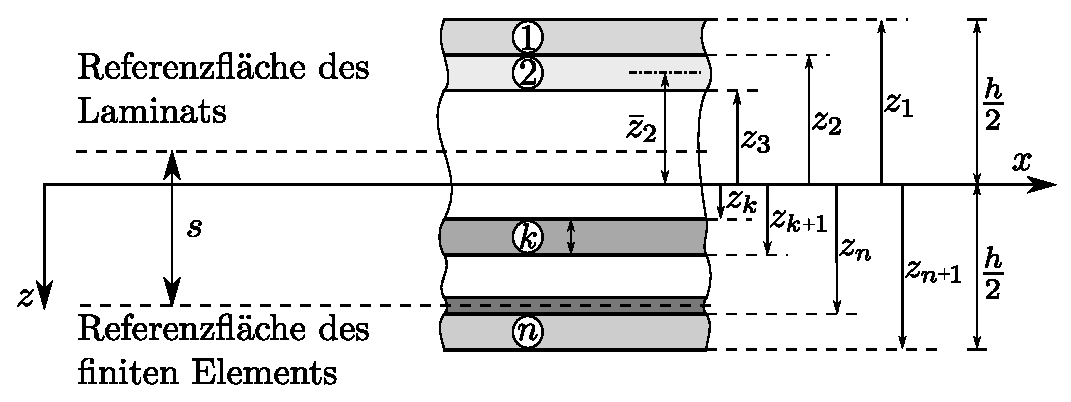
\includegraphics[scale=0.6]{Bilder/Laminatshift}
		\end{center}
 		\caption{Verschiebung von Material- und Elementreferenzebene nach \cite{Gei1999_p1} \label{Abb_Laminatshift}}
 		\end{figure}
\item Die entsprechenden Einträge lassen sich definieren, werden jedoch in der derzeitigen Version nicht in der Berechnung genutzt.
\end{enumerate}

\subsubsection{To-Do-Liste am Eintrag}

\begin{itemize}
\item ...
\end{itemize}

\newpage

\subsection{PBeam}

\subsubsection{Beschreibung}

Diese Karte definiert die Eigenschaften eines Balkenelements mit isotropem Materialmodell.\\
Die Datei muss den Namen \emph{pbeam.fipps} haben.

\subsubsection{Input-Karte}

\begin{table}[htbp]
\centering
\begin{tabularx}{\textwidth}{cCCCCCCCC}
\toprule
Karte 1	& 1		& 2		& 3		& 4		& 5		& 6		& 7		& 8		\\
\midrule
Variable& pid		& mid		& AA		& I11		& I22		& I12		& It		& t1		\\
Type	& I>0		& I>0		& R$\ge$0.0	& R$\ge$0.0	& R$\ge$0.0	& R$\ge$0.0	& R$\ge$0.0	& R$\ge$0.0	\\
Default	& -		& -		& -		& -		& -		& -		& Ip		& -		\\
Remark	& 1		& -		& -		& -		& -		& 2		& 3		& 4		\\
aktuell	& \multirow{2}{*}{\checkmark}	& \multirow{2}{*}{\checkmark}	& \multirow{2}{*}{\checkmark}	& \multirow{2}{*}{\checkmark}	& \multirow{2}{*}{\checkmark}	& \multirow{2}{*}{\checkmark}	& \multirow{2}{*}{\checkmark}	& \multirow{2}{*}{\checkmark}	\\
genutzt \\
\\
Karte 2	& 9		& 10		& 11		& 12		& 13		& 14		& 15		& 16		\\
\midrule
Variable& t2		& angle		& atype		& nsm		& -			& -			& -			& -			\\
Type	& R$\ge$0.0	& R		& C		& R$\ge$0.0	& -			& -			& -			& -			\\
Default	& -		& -		& -		& -		& -			& -			& -			& -			\\
Remark	& 4		& -		& -		& 5		& -			& -			& -			& -			\\
aktuell	& \multirow{2}{*}{\checkmark}	& \multirow{2}{*}{\checkmark}	& \multirow{2}{*}{\checkmark}	& \multirow{2}{*}{-}	& \multirow{2}{*}{-}	& \multirow{2}{*}{-}	& \multirow{2}{*}{-}	& \multirow{2}{*}{-}	\\
genutzt \\
\bottomrule
\end{tabularx}
% \caption{FiPPS Input-Karte für die Eigenschaften eines Balkenelements mit isotropem Materialmodell \label{Tab_Inp_PBeam}}
\end{table}

\subsubsection{Beschreibung}

\begin{tabularx}{\textwidth}{cXcc}
\toprule
Variable& Beschreibung											& Typ			& Format\\
\midrule
pid	& Property-ID											& Integer > 0		& I10	\\
mid	& Material-ID (Mat1-Karte)									& Integer > 0		& I10	\\
AA	& Fläche des Balkenquerschnitts									& Real $\ge$ 0.0	& E23.16\\
I11	& Flächenträgheitsmoment des Querschnitts um z-Hauptachse (=Izz)				& Real $\ge$ 0.0	& E23.16\\
I22	& Flächenträgheitsmoment des Querschnitts um y-Hauptachse (=Iyy)				& Real $\ge$ 0.0	& E23.16\\
I12	& Deviationsmoment des Querschnitts (=Izy)							& Real $\ge$ 0.0	& E23.16\\
It	& Torsionsflächenträgheitsmoment des Querschnitts						& Real $\ge$ 0.0	& E23.16\\
t1	& Dicke in z-Richtung										& Real $\ge$ 0.0	& E23.16\\
t2	& Dicke in y-Richtung										& Real $\ge$ 0.0	& E23.16\\
angle	& Winkel zwischen Hauptachsensystem und lokalem kartesischen Koordinatensystem des Balkens	& Real			& E23.16\\
atype	& Winkeltyp, 'deg' or 'rad'									& Character		& 3A	\\
nsm	& Non-structural mass per unit area								& Real $\ge$ 0.0	& E23.16\\
\bottomrule
\end{tabularx}

\subsubsection{Hinweise}

\begin{enumerate}
\item Die Property-ID's (pid) dürfen für die gesamte Anzahl an verwendeten Properties nur einmalig genutzt werden. Demzufolge darf es keine PShell-ID 1 und PComp-ID 1 in einem Modell gleichzeitig geben.
\item Es sind alle Werte zulässig, die die Ungleichung $I11\cdot I22-I12^2>0,0$ erfüllen.
\item Wird kein Torsionsflächenträgheitsmoment angegeben, wird für die Berechnungen das polare Flächenträgheitsmoment genutzt (Ip=I11+I22).
\item Die angegebenen Dicken werden zur Berechnung der maximal im Querschnitt auftretenden Spannungen benötigt und geben die maximalen Abstände des Querschnitts von dessen Schwerpunkt an. Sie gehen nicht in die Berechnung der Steifigkeitsmatrizen der Elemente ein.
\item Die entsprechenden Einträge lassen sich definieren, werden jedoch in der derzeitigen Version nicht in der Berechnung genutzt.
\end{enumerate}

\subsubsection{To-Do-Liste am Eintrag}

\begin{itemize}
\item ...
\end{itemize}

\newpage

\subsection{PLsolid}

\subsubsection{Beschreibung}

Die Eingabekarte definiert die Eigenschaften des Layered Solid-Elements Lsolid20 für mehrschichtige Laminate orthotroper Einzellagen.\\
Die Datei muss den Namen \emph{plsolid.fipps} haben.

\subsubsection{Input-Karte}

\begin{table}[htbp]
\centering
\begin{tabularx}{\textwidth}{cCCCCCCCC}
\toprule
Karte 1         & 1     & 2      & 3     & 4  & 5  & 6  & 7  & 8   \\
\midrule
Variable        & pid   & lamid  & cid   & res"-Lay  & glob"-Out  & -  & -  & -   \\
Typ             & I>0   & I>0    & I$\geq\!-1$   & I $\geq$ 0 & L  & -  & -  & -   \\
Standard        & -     & -      & 0     & 0  & F  & -  & -  & -   \\
Hinweis         & -     & -      & 1     & 2  & 3  & -  & -  & -   \\
aktuell        & \multirow{2}{*}{\checkmark} & \multirow{2}{*}{\checkmark} & \multirow{2}{*}{\checkmark} & \multirow{2}{*}{\checkmark}  & \multirow{2}{*}{\checkmark}  & \multirow{2}{*}{-}  & \multirow{2}{*}{-}  & \multirow{2}{*}{-}   \\
genutzt \\
\bottomrule
\end{tabularx}
\end{table}

\subsubsection{Beschreibung}

\begin{tabularx}{\textwidth}{cXcc}
\toprule
Variable  & Beschreibung  & Typ          & Format  \\
\midrule
pid       & Property-ID   & Integer > 0  & I10     \\
lamid     & Laminat-ID    & Integer > 0  & I10     \\
cid       & Koordinatensystem-ID  & Integer $\geq -1$  & I10     \\
resLay    & Lagennummer, für die Spannungen und Dehnungen ausgegeben werden & Integer $\geq 0$ & I10 \\
globOut   & Optionale Ausgabe im globalen Koordinatensystem & Logical & L1 \\
\bottomrule
\end{tabularx}

\subsubsection{Hinweise}

\begin{enumerate}
 \item Die x-Achse des Koordinatensystems gibt die Orientierung der x-Achse und damit der Fasernullrichtung des Elementkoordinatensystems vor. Hierzu wird die x-Achse des Koordinatensystems in die Elementmittenebene projiziert. Mit dem Standardwert cid~= 0 erfolgt die Orientierung des Elementkoordinatensystems nur nach der Elementorientierung, sodass die x-Achse der $\xi$-Koordinate folgt. Mit cid~= $-1$ wird die x-Achse des globalen Koordinatensystems zur Orientierung genutzt.
 \item Gibt die Nummer der Lage an, für die die Spannungen und Verzerrungen ausgegeben werden. Ist resLay~= 0, erfolgt die Ausgabe an der Oberseite der obersten Lage und an der Unterseite der untersten Lage im Elementkoordinatensystem. Andernfalls werden die Werte an der Ober- und Unterseite der jeweiligen Lage im entsprechenden Materialkoordinatensystem ausgegeben. Ist nur ein Integrationspunkt über der Lagendicke vorhanden, erfolgt die Darstellung der Werte in der Lagenmitte.
 \item Ist der Schalter globOut auf \textit{true} gesetzt, erfolgt die Ausgabe der Spannungen und Verzerrungen im globalen Koordinatensystem. Ist der Schalter auf \textit{false} gesetzt, erfolgt die Ausgabe im Element- oder Materialkoordinatensystem (vergleiche Hinweis 2). Ohne Eintrag erfolgt die Ausgabe standardmäßig im Elementkoordinatensystem.
\end{enumerate}

\newpage

\section{Randbedingungen}

\subsection{Coupling}

\subsubsection{Beschreibung}

Diese Karte definiert Sets von Knoten, für die Freiheiten miteinander gekoppelt werden.\\
Die Datei muss den Namen \emph{couplings.fipps} haben.

\subsubsection{Input-Karte}

\begin{table}[htbp]
\centering
\begin{tabularx}{\textwidth}{cCCCCCCCC}
\toprule
Karte 1	& 1		& 2		& 3		& 4		& 5		& 6		& 7		& 8		\\
\midrule
Variable& cpsid		& dof		& nid		& -		& -		& -		& -		& -		\\
Typ	& I>0		& I>0		& I>0		& -		& -		& -		& -		& -		\\
Standard& -		& -		& -		& -		& -		& -		& -		& -		\\
Hinweis	& 1		& 2		& -		& -		& -		& -		& -		& -		\\
aktuell	& \multirow{2}{*}{\checkmark}	& \multirow{2}{*}{\checkmark}	& \multirow{2}{*}{\checkmark}	& \multirow{2}{*}{-}	& \multirow{2}{*}{-}	& \multirow{2}{*}{-}	& \multirow{2}{*}{-}	& \multirow{2}{*}{-}	\\
genutzt \\
\bottomrule
\end{tabularx}
% \caption{FiPPS Input-Karte für die Eigenschaften eines Sets von Randbedingungen \label{Tab_Inp_Spcadd}}
\end{table}

\subsubsection{Beschreibung}

\begin{tabularx}{\textwidth}{cXcc}
\toprule
Variable& Beschreibung		& Typ		& Format\\
\midrule
cpsid	& Coupling-Set-ID	& Integer > 0	& I10	\\
dof	& zu koppelnder Freiheitsgrad		& Integer > 0	& I10	\\
nid	& Knoten-ID		& Integer > 0	& I10	\\
\bottomrule
\end{tabularx}

\subsubsection{Hinweise}

\begin{enumerate}
\item Für alle Freiheiten, die miteinander gekoppelt werden sollen, muss die Coupling-Set-ID (cpsid) gleich sein.
\item Es darf immer nur ein Freiheitsgrad angegeben werden.
\end{enumerate}

\subsubsection{To-Do-Liste am Eintrag}

\begin{itemize}
\item ...
\end{itemize}

\newpage

\subsection{Spcadd}

\subsubsection{Beschreibung}

Diese Karte definiert Set von Randbedingungen.\\
Die Datei muss den Namen \emph{spcadd.fipps} haben.

\subsubsection{Input-Karte}

\begin{table}[htbp]
\centering
\begin{tabularx}{\textwidth}{cCCCCCCCC}
\toprule
Karte 1	& 1		& 2		& 3		& 4		& 5		& 6		& 7		& 8		\\
\midrule
Variable& scid		& sid		& -		& -		& -		& -		& -		& -		\\
Typ	& I>0		& I>0		& -		& -		& -		& -		& -		& -		\\
Standard& -		& -		& -		& -		& -		& -		& -		& -		\\
Hinweis	& 1		& -		& -		& -		& -		& -		& -		& -		\\
aktuell	& \multirow{2}{*}{\checkmark}	& \multirow{2}{*}{\checkmark}	& \multirow{2}{*}{-}	& \multirow{2}{*}{-}	& \multirow{2}{*}{-}	& \multirow{2}{*}{-}	& \multirow{2}{*}{-}	& \multirow{2}{*}{-}	\\
genutzt \\
\bottomrule
\end{tabularx}
% \caption{FiPPS Input-Karte für die Eigenschaften eines Sets von Randbedingungen \label{Tab_Inp_Spcadd}}
\end{table}

\subsubsection{Beschreibung}

\begin{tabularx}{\textwidth}{cXcc}
\toprule
Variable& Beschreibung		& Typ		& Format\\
\midrule
scid	& Spc-Set-ID		& Integer > 0	& I10	\\
sid	& Spc-ID		& Integer > 0	& I10	\\
\bottomrule
\end{tabularx}

\subsubsection{Hinweise}

\begin{enumerate}
\item ...
\end{enumerate}

\subsubsection{To-Do-Liste am Eintrag}

\begin{itemize}
\item Über Bezeichungen Scid und Sid nachdenken (Sid könnte auch set-id sein)
\end{itemize}

\newpage

\subsection{Spc1}

\subsubsection{Beschreibung}

Diese Karte definiert eine homogene Verschiebungsrandbedingung im globalen Koordinatensystem.\\
Die Datei muss den Namen \emph{spc1.fipps} haben.

\subsubsection{Input-Karte}

\begin{table}[htbp]
\centering
\begin{tabularx}{\textwidth}{cCCCCCCCC}
\toprule
Karte 1	& 1		& 2		& 3		& 4		& 5		& 6		& 7		& 8		\\
\midrule
Variable& sid		& dof		& n1		& thru		& nn		& inc		& -		& -		\\
Typ	& I>0		& I>0		& I>0		& L		& I>0		& I>0		& -		& -		\\
Standard& -		& -		& -		& -		& -		& 1		& -		& -		\\
Hinweis	& 1		& -		& -		& -		& -		& 2		& -		& -		\\
aktuell	& \multirow{2}{*}{\checkmark}	& \multirow{2}{*}{\checkmark}	& \multirow{2}{*}{\checkmark}	& \multirow{2}{*}{\checkmark}	& \multirow{2}{*}{\checkmark}	& \multirow{2}{*}{-}	& \multirow{2}{*}{-}	& \multirow{2}{*}{-}	\\
genutzt \\
\bottomrule
\end{tabularx}
% \caption{FiPPS Input-Karte für die eine homogene Verschiebungsrandbedingungen \label{Tab_Inp_Spc1}}
\end{table}

\subsubsection{Beschreibung}

\begin{tabularx}{\textwidth}{cXcc}
\toprule
Variable& Beschreibung												& Typ		& Format\\
\midrule
sid	& Spc-ID												& Integer > 0	& I10	\\
dof	& Gesperrte Freiheitsgrade. Jede Kombination der Werte 1 bis 6 ohne Leerzeichen und doppelte Zahlen. Die Reihenfolge der Werte spielt keine Rolle. Zur Sperrung aller Translationen muss somit die Kombination 123 eingetragen werden. Zur Sperrung von allen statischen Freiheitsgraden eines Knotens (drei Translationen und drei Rotationen) muss die Kombination 123456 eingetragen werden.														& Integer > 0	& I10	\\
n1	& Knoten-ID des ersten Knotens an dem die Randbedingung wirken soll					& Integer > 0	& I10	\\
thru	& Logischer Operator, wenn \emph{true} dann wird die Randbedingung auf die Knoten von n1 bis n2 aufgebracht, wenn \emph{false} wirkt die Randbedingung nur auf dem Knoten mit n1.																& Logical	& L1	\\
nn	& Wenn thru=\emph{true} Knoten-ID des Knotens bis zu dem die Randbedingung aufgebracht werden soll.	& Integer > 0	& I10	\\
inc	& Inkrement der Knotennummern zwischen n1 und nn auf dem die Randbedingung aufgebracht werden soll.	& Integer > 0	& I10	\\
\bottomrule
\end{tabularx}

\subsubsection{Hinweise}

\begin{enumerate}
\item Die Spc-ID's (sid) dürfen für die gesamte Anzahl an verwendeten Randbedingungen nur einmalig genutzt werden. Demzufolge darf es keine Spc1-ID 1 und Spcd-ID 1 in einem Modell gleichzeitig geben.
\item Dieser Wert wird in der aktuellen Version in der Berechnung nicht berücksichtigt.
\end{enumerate}

\subsubsection{To-Do-Liste am Eintrag}

\begin{itemize}
\item Die Bezeichnung n1 und nn in nid1 und nid2 ändern entsprechend Bezeichnung bei thru wie in p3load.
\item inc implementieren.
\end{itemize}

\newpage

\subsection{Spcd}

\subsubsection{Beschreibung}

\textbf{Diese Karte ist derzeit nicht implementiert.}

Diese Karte definiert eine inhomogene Verschiebungsrandbedingung im globalen Koordinatensystem.\\
Die Datei muss den Namen \emph{spcd.fipps} haben.

\subsubsection{Input-Karte}

\begin{table}[htbp]
\centering
\begin{tabularx}{\textwidth}{cCCCCCCCC}
\toprule
Karte 1	& 1		& 2		& 3		& 4		& 5		& 6		& 7		& 8		\\
\midrule
Variable& sid		& nid		& dof		& val		& -		& -		& -		& -		\\
Typ	& I>0		& I>0		& 1$\le$I$\le$6	& R		& -		& -		& -		& -		\\
Standard& -		& -		& -		& -		& -		& -		& -		& -		\\
Hinweis	& 1		& -		& -		& -		& -		& -		& -		& -		\\
aktuell	& \multirow{2}{*}{\checkmark}	& \multirow{2}{*}{\checkmark}	& \multirow{2}{*}{\checkmark}	& \multirow{2}{*}{\checkmark}	& \multirow{2}{*}{-}	& \multirow{2}{*}{-}	& \multirow{2}{*}{-}	& \multirow{2}{*}{-}	\\
genutzt \\
\bottomrule
\end{tabularx}
% \caption{FiPPS Input-Karte für die eine inhomogene Verschiebungsrandbedingungen \label{Tab_Inp_Spcd}}
\end{table}

\subsubsection{Beschreibung}

\begin{tabularx}{\textwidth}{cXcc}
\toprule
Variable& Beschreibung												& Typ				& Format\\
\midrule
sid	& Spc-ID												& Integer > 0			& I10	\\
nid	& Knoten-ID	des Knotens auf den die inhomogene Verschiebungsrandbedingung aufgebracht werden soll.	& Integer > 0			& I10	\\
dof	& Freiheitsgrad mit vorgeschriebenem Wert. Zahl von 1 bis 6.						& 1 $\le$ Integer  $\le$ 6	& I10	\\
val	& Größe der vorgeschriebenen Bewegung									& Real				& E23.16\\
\bottomrule
\end{tabularx}

\subsubsection{Hinweise}

\begin{enumerate}
\item Die Spc-ID's (sid) dürfen für die gesamte Anzahl an verwendeten Randbedingungen nur einmalig genutzt werden. Demzufolge darf es keine Spc1-ID 1 und Spcd-ID 1 in einem Modell gleichzeitig geben.
\end{enumerate}

\subsubsection{To-Do-Liste am Eintrag}

\begin{itemize}
\item ...
\end{itemize}

\newpage

\subsection{Mpcadd}

\subsubsection{Beschreibung}

Diese Karte definiert Set von Multi Point Constraints.\\
Die Datei muss den Namen \emph{mpcadd.fipps} haben.

\subsubsection{Input-Karte}

\begin{table}[htbp]
\centering
\begin{tabularx}{\textwidth}{cCCCCCCCC}
\toprule
Karte 1	& 1		& 2		& 3		& 4		& 5		& 6		& 7		& 8		\\
\midrule
Variable& scid		& sid		& -		& -		& -		& -		& -		& -		\\
Typ	& I>0		& I>0		& -		& -		& -		& -		& -		& -		\\
Standard& -		& -		& -		& -		& -		& -		& -		& -		\\
Hinweis	& -		& -		& -		& -		& -		& -		& -		& -		\\
aktuell	& \multirow{2}{*}{\checkmark}	& \multirow{2}{*}{\checkmark}	& \multirow{2}{*}{-}	& \multirow{2}{*}{-}	& \multirow{2}{*}{-}	& \multirow{2}{*}{-}	& \multirow{2}{*}{-}	& \multirow{2}{*}{-}	\\
genutzt \\
\bottomrule
\end{tabularx}
% \caption{FiPPS Input-Karte für die Eigenschaften eines Sets von Randbedingungen \label{Tab_Inp_Spcadd}}
\end{table}

\subsubsection{Beschreibung}

\begin{tabularx}{\textwidth}{cXcc}
\toprule
Variable& Beschreibung		& Typ		& Format\\
\midrule
scid	& Mpc-Set-ID		& Integer > 0	& I10	\\
sid	& Mpc-ID		& Integer > 0	& I10	\\
\bottomrule
\end{tabularx}

\subsubsection{Hinweise}

\begin{enumerate}
\item ...
\end{enumerate}

\subsubsection{To-Do-Liste am Eintrag}

\begin{itemize}
\item Über Bezeichungen Scid und Sid nachdenken (Sid könnte auch set-id sein)
\end{itemize}

\newpage

\subsection{Mpc}

\subsubsection{Beschreibung}

Diese Karte definiert ein Multi Point Constraint der Form\\
\begin{equation}
 0 = fac^s u^s + \sum_i fac^m_i u^m_i
\end{equation}
im Knotenkoordinatensystem.\\
Die Datei muss den Namen \emph{mpc.fipps} haben. \\
\\
Achtung!!: Im Gegensatz zu allen anderen Karten ist diese zweizeilig pro Eintrag.

\subsubsection{Input-Karte}

\begin{table}[htbp]
\centering
\begin{tabularx}{\textwidth}{cCCCCCCCC}
\toprule
Zeile 1	& 1		& 2		& 3		& 4		& 5		& 6		& 7	& 8	\\
\midrule
Variable& nmdof		& snid		& sdof		& sfac		& -		& -		& -	& -	\\
Typ	& I>0		& I>0		& I>0		& R		& -		& -		& -	& -	\\
Standard& -		& -		& -		& -		& -		& -		& -	& -	\\
Hinweis	& -		& -		& 1		& -		& -		& -		& -	& -	\\
aktuell	& \multirow{2}{*}{\checkmark}	& \multirow{2}{*}{\checkmark}	& \multirow{2}{*}{\checkmark}	& \multirow{2}{*}{\checkmark}	& \multirow{2}{*}{-}	& \multirow{2}{*}{-}	& \multirow{2}{*}{-}	& \multirow{2}{*}{-}	\\
genutzt \\
\bottomrule
\end{tabularx}
% \caption{FiPPS Input-Karte für die eine homogene Verschiebungsrandbedingungen \label{Tab_Inp_Spc1}}
\end{table}

\begin{table}[htbp]
\centering
\begin{tabularx}{\textwidth}{cCCCCCCCC}
\toprule
Zeile 2	& 1		& 2		& 3		& 4		&  5		&  6		&  ...		&  		\\
\midrule
Variable& mnid1		& mdof1		& mfac1		& mnid2		&  mdof2	&  mfac2	&  ...		&  		\\
Typ	& I>0		& I>0		& R		& I>0		&  I>0		&  R		&  ...		&  		\\
Standard& -		& -		& -		& -		&  -		&  -		&  ...		&  		\\
Hinweis	& -		& 1		& -		& -		&  -		&  -		&  2		&  		\\
aktuell	& \multirow{2}{*}{\checkmark}	& \multirow{2}{*}{\checkmark}	& \multirow{2}{*}{\checkmark}	&  \multirow{2}{*}{\checkmark}	&  \multirow{2}{*}{\checkmark}	&  \multirow{2}{*}{\checkmark}	&  \multirow{2}{*}{\checkmark}	&  	\\
genutzt \\
\bottomrule
\end{tabularx}
% \caption{FiPPS Input-Karte für die eine homogene Verschiebungsrandbedingungen \label{Tab_Inp_Spc1}}
\end{table}

\subsubsection{Beschreibung}

\begin{tabularx}{\textwidth}{cXcc}
\toprule
Variable& Beschreibung												& Typ		& Format \\
\midrule
nmdof	& Anzahl der unabhängigen Freiheiten (entsprechend viele Einträge müssen in der zweiten Zeile erfolgen)	& Integer > 0	& I10	 \\
snid	& Knoten-ID des abhängigen Knotens									& Integer > 0	& I10	 \\
sdof	& zu koppelnde Freiheit des abhängigen Knotens								& Integer > 0	& I10    \\
sfac	& Faktor für die Freiheit des abhängigen Knotens							& Real		& E23.16 \\
mnidi	& Knoten-ID des i-ten unabhängigen Knotens								& Integer > 0	& I10	 \\
mdofi	& zu koppelnde Freiheit des i-ten unabhängigen Knotens 							& Integer > 0	& I10	 \\
mfaci	& Faktor für die Freiheit des i-ten unabhängigen Knotens						& Real		& E23.16 \\
\bottomrule
\end{tabularx}

\subsubsection{Hinweise}

\begin{enumerate}
\item Es darf immer nur ein Freiheitsgrad angegeben werden.
\item Die Einträge mnid, mdof und mfac müssen nmdof-mal vorhanden sein.
\end{enumerate}

\subsubsection{To-Do-Liste am Eintrag}

\begin{itemize}
\item ...
\end{itemize}

\newpage

\section{Kontakte}

\subsection{Knoten-Beam2-Kontakt}

\subsubsection{Beschreibung}

Diese Karte definiert einen starren Kontakt zwischen einem Knoten und einem Beam2"=Ele"-ment. Dabei wird der Knoten auf die Elementachse, unter Berücksichtigung der vorzugebenden Elementkoordinate, verschoben. Der Knoten ist anschließend starr mit der Elementachse verbunden und bewegt sich mit dieser. Der Kontakt wird über die Ansatzfunktion des Beam2-Elements und interne MPCs realisiert.\\
Die Translationen und Rotationen des abhängigen Knoten werden jeweils über die Ansatzfunktion des Beam2-Elements aus den Freiheiten der unabhängigen Knoten gemittelt. Hierbei ist zu beachten, dass dem Balkenelement ein kubischer Ansatz für die Durchbiegung in Richtung der y- und z-Achse des Elementkoordinatensystems zugrunde liegt. Daher kann der Knoten bei der Darstellung des Balkens als lineares Element deutlich außerhalb des verformten Elements dargestellt werden.\\
Die Datei muss den Namen \emph{contact\_node\_beam2.fipps} haben.

\subsubsection{Input-Karte}

\begin{table}[htbp]
\centering
\begin{tabularx}{\textwidth}{cCCCCCCCC}
\toprule
Karte 1	& 1		& 2		& 3		& 4		& 5		& 6		& 7		& 8		\\
\midrule
Variable& eid		& nid		& xi		& -		& -		& -		& -		& -		\\
Typ	& I>0		& I>0		& R		& -		& -		& -		& -		& -		\\
Standard& -		& -		& -		& -		& -		& -		& -		& -		\\
Hinweis	& -		& 1		& -		& -		& -		& -		& -		& -		\\
aktuell	& \multirow{2}{*}{\checkmark}	& \multirow{2}{*}{\checkmark}	& \multirow{2}{*}{\checkmark}	& \multirow{2}{*}{-}	& \multirow{2}{*}{-}	& \multirow{2}{*}{-}	& \multirow{2}{*}{-}	& \multirow{2}{*}{-}	\\
genutzt \\
\bottomrule
\end{tabularx}
% \caption{FiPPS Input-Karte für die Eigenschaften eines Sets von Randbedingungen \label{Tab_Inp_Spcadd}}
\end{table}

\subsubsection{Beschreibung}

\begin{tabularx}{\textwidth}{cXcc}
\toprule
Variable& Beschreibung				& Typ		& Format\\
\midrule
eid	& Element-ID des Beam2-Elements		& Integer > 0	& I10	\\
nid	& Knoten-ID				& Integer > 0	& I10	\\
xi	& Knotenposition in Elementkoordinaten	& Real		& E23.16	\\
\bottomrule
\end{tabularx}

\subsubsection{Hinweise}

\begin{enumerate}
\item Derzeit darf diesem Knoten keine weitere Randbedingung (Verschiebung, Kräfte) zugeordnet sein.
\end{enumerate}

\subsubsection{To-Do-Liste am Eintrag}

\begin{itemize}
\item Klären, was mit weiteren Randbedingungen auf die Knoten passiert.
\end{itemize}

\newpage

\subsection{Knoten-Quad8-Kontakt}

\subsubsection{Beschreibung}

Diese Karte definiert einen starren Kontakt zwischen einem Knoten und einem Quad8-Element. Dabei wird zunächst die Normale auf der Elementmittelfläche bestimmt, die durch den Knoten verläuft. Anschließend wird der Knoten auf die Elementmittelfläche verschoben. Der Knoten ist abschließend starr mit der Elementmittelfläche verbunden und bewegt sich mit dieser. Der Kontakt wird über die Ansatzfunktionen des Quad8-Elements und interne MPCs realisiert.\\
Es werden die Translationen und Rotationen des abhängigen Knoten jeweils über die Ansatzfunktionen des Quad8-Elements aus den Freiheiten der unabhängigen Knoten gemittelt.\\
Die Datei muss den Namen \emph{contact\_node\_quad8.fipps} haben.

\subsubsection{Input-Karte}

\begin{table}[htbp]
\centering
\begin{tabularx}{\textwidth}{cCCCCCCCC}
\toprule
Karte 1	& 1		& 2		& 3		& 4		& 5		& 6		& 7		& 8		\\
\midrule
Variable& eid		& nid		& -		& -		& -		& -		& -		& -		\\
Typ	& I>0		& I>0		& -		& -		& -		& -		& -		& -		\\
Standard& -		& -		& -		& -		& -		& -		& -		& -		\\
Hinweis	& -		& 1		& -		& -		& -		& -		& -		& -		\\
aktuell	& \multirow{2}{*}{\checkmark}	& \multirow{2}{*}{\checkmark}	& \multirow{2}{*}{\checkmark}	& \multirow{2}{*}{-}	& \multirow{2}{*}{-}	& \multirow{2}{*}{-}	& \multirow{2}{*}{-}	& \multirow{2}{*}{-}	\\
genutzt \\
\bottomrule
\end{tabularx}
% \caption{FiPPS Input-Karte für die Eigenschaften eines Sets von Randbedingungen \label{Tab_Inp_Spcadd}}
\end{table}

\subsubsection{Beschreibung}

\begin{tabularx}{\textwidth}{cXcc}
\toprule
Variable& Beschreibung				& Typ		& Format\\
\midrule
eid	& Element-ID des Quad8-Elements		& Integer > 0	& I10	\\
nid	& Knoten-ID				& Integer > 0	& I10	\\
\bottomrule
\end{tabularx}

\subsubsection{Hinweise}

\begin{enumerate}
\item Derzeit darf diesem Knoten keine weitere Randbedingung (Verschiebung, Kräfte) zugeordnet sein.
\end{enumerate}

\subsubsection{To-Do-Liste am Eintrag}

\begin{itemize}
\item Klären, was mit weiteren Randbedingungen auf die Knoten passiert.
\end{itemize}

\newpage

\subsection{Knoten-Lsolid20-Kontakt}

\subsubsection{Beschreibung}

Diese Karte definiert einen starren Kontakt zwischen einem Knoten und einem Lsolid20"=Element. Dabei werden zunächst die natürlichen Elementkoordinaten des zu koppelnden Knotens ermittelt. Dieser kann auch außerhalb des Elements liegen und wird nicht verschoben. Liegt der zu koppelnde Knoten außerhalb des Elements, erfolgt die Ausgabe eines Warnhinweises. Anschließend erfolgt die Realisierung des Kontakts über die Ansatzfunktionen des Lsolid20"=Elements und interne MPCs.\\
Die Translationen des abhängigen Knoten werden damit jeweils über die Ansatzfunktionen des Lsolid20-Elements aus den Translationen der unabhängigen Knoten gemittelt. Es werden keine Abhängigkeiten für die Rotationen des abhängigen Knotens generiert. Diese sind daher separat zu sperren, sofern der kontaktierte Knoten nicht Teil eines Lsolid20"=Elements ist.\\
Die Datei muss den Namen \emph{contact\_node\_lsolid20.fipps} haben.

\subsubsection{Input-Karte}

\begin{table}[htbp]
\centering
\begin{tabularx}{\textwidth}{cCCCCCCCC}
\toprule
Karte 1	& 1		& 2		& 3		& 4		& 5		& 6		& 7		& 8		\\
\midrule
Variable& eid		& nid		& -		& -		& -		& -		& -		& -		\\
Typ	& I>0		& I>0		& -		& -		& -		& -		& -		& -		\\
Standard& -		& -		& -		& -		& -		& -		& -		& -		\\
Hinweis	& -		& 1		& -		& -		& -		& -		& -		& -		\\
aktuell	& \multirow{2}{*}{\checkmark}	& \multirow{2}{*}{\checkmark}	& \multirow{2}{*}{\checkmark}	& \multirow{2}{*}{-}	& \multirow{2}{*}{-}	& \multirow{2}{*}{-}	& \multirow{2}{*}{-}	& \multirow{2}{*}{-}	\\
genutzt \\
\bottomrule
\end{tabularx}
% \caption{FiPPS Input-Karte für die Eigenschaften eines Sets von Randbedingungen \label{Tab_Inp_Spcadd}}
\end{table}

\subsubsection{Beschreibung}

\begin{tabularx}{\textwidth}{cXcc}
\toprule
Variable& Beschreibung				& Typ		& Format\\
\midrule
eid	& Element-ID des Lsolid20-Elements		& Integer > 0	& I10	\\
nid	& Knoten-ID				& Integer > 0	& I10	\\
\bottomrule
\end{tabularx}

\subsubsection{Hinweise}

\begin{enumerate}
\item Derzeit darf diesem Knoten keine weitere Randbedingung (Verschiebung, Kräfte) zugeordnet sein.
\end{enumerate}

\subsubsection{To-Do-Liste am Eintrag}

\begin{itemize}
\item Klären, was mit weiteren Randbedingungen auf die Knoten passiert.
\end{itemize}

\newpage

\section{Koordinatensysteme}

\subsection{Coords}

\subsubsection{Beschreibung}

Diese Karte definiert ein lokales kartesisches Koordinatensystem.\\
Die Datei muss den Namen \emph{coord.fipps} haben.

\subsubsection{Input-Karte}

\begin{table}[htbp]
\centering
\begin{tabularx}{\textwidth}{cCCCCCCCC}
\toprule
Karte 1	& 1		& 2		& 3		& 4		& 5		& 6		& 7		& 8		\\
\midrule
Variable& cid		& xAxisVec1	& xAxisVec2	& xAxisVec3	& yAxisVec1	& yAxisVec2	& yAxisVec3	& zAxisVec1	\\
Typ	& I>0		& R		& R		& R		& R		& R		& R		& -		\\
Standard& -		& -		& -		& -		& -		& -		& -		& -		\\
Hinweis	& 1		& 1		& 1		& 1		& 1		& 1		& 1		& 1		\\
aktuell	& \multirow{2}{*}{\checkmark}	& \multirow{2}{*}{\checkmark}	& \multirow{2}{*}{\checkmark}	& \multirow{2}{*}{\checkmark}	& \multirow{2}{*}{\checkmark}	& \multirow{2}{*}{\checkmark}	& \multirow{2}{*}{\checkmark}	& \multirow{2}{*}{\checkmark}	\\
genutzt \\
\\
Karte 1	& 9		& 10		& 11		& 12		& 13		& 14		& 15		& 16		\\
\midrule
Variable& zAxisVec2	& zAxisVec3	& -		& -		& -		& -		& -		& -		\\
Typ	& R		& R		& -		& -		& -		& -		& -		& -		\\
Standard& -		& -		& -		& -		& -		& -		& -		& -		\\
Hinweis	& 1		& 1		& -		& -		& -		& -		& -		& -		\\
aktuell	& \multirow{2}{*}{\checkmark}	& \multirow{2}{*}{\checkmark}	& \multirow{2}{*}{-}	& \multirow{2}{*}{-}	& \multirow{2}{*}{-}	& \multirow{2}{*}{-}	& \multirow{2}{*}{-}	& \multirow{2}{*}{-}	\\
genutzt \\
\bottomrule
\end{tabularx}
% \caption{FiPPS Input-Karte für die Definition eines lokalen kartesischen Koordinatensystems \label{Tab_Inp_Coord}}
\end{table}

\subsubsection{Beschreibung}

\begin{tabularx}{\textwidth}{cXcc}
\toprule
Variable	& Beschreibung								& Typ		& Format	\\
\midrule
cid		& Koordinatensystem-ID							& Integer > 0	& I10		\\
xAxisVeci	& Vektor-Komponenten der x-Achse des lokalen Koordinatensystems (Hinweis 1 beachten)	& Real		& 3E23.16	\\
yAxisVeci	& Vektor-Komponenten der y-Achse des lokalen Koordinatensystems (Hinweis 1 beachten)	& Real		& 3E23.16	\\
zAxisVeci	& Vektor-Komponenten der z-Achse des lokalen Koordinatensystems (Hinweis 1 beachten)	& Real		& 3E23.16	\\
\bottomrule
\end{tabularx}

\subsubsection{Hinweise}

\begin{enumerate}
\item Die drei Vektoren müssen normiert sein.
\end{enumerate}

\subsubsection{To-Do-Liste am Eintrag}

\begin{itemize}
\item ...
\end{itemize}

\newpage

\section{Subcases}
\label{sec:subcase}

\subsection{Subcase}

\subsubsection{Beschreibung}

Diese Karte definiert einen Subcase - die Kombination von Lastfall und Lagerung.\\
Die Datei muss den Namen \emph{subcase.fipps} haben.

\subsubsection{Input-Karte}

\begin{table}[htbp]
\centering
\begin{tabularx}{\textwidth}{cCCCCCCCC}
\toprule
Karte 1	& 1		& 2		& 3		& 4		& 5		& 6		& 7		& 8		\\
\midrule
Variable& scid		& spcaddid	& loadid	& mpcaddid	& skip"-Buckling& upgeom	& upstress	& output	\\
Typ	& I>0		& I>0		& I>0		& I>0		& L		& L		& L		& L		\\
Standard& -		& -		& -		& -		& -		& -		& -		& -		\\
Hinweis	& -		& -		& -		& -		& -		& -		& -		& -		\\
aktuell	& \multirow{2}{*}{\checkmark}	& \multirow{2}{*}{\checkmark}	& \multirow{2}{*}{\checkmark}	& \multirow{2}{*}{\checkmark}	& \multirow{2}{*}{-}	& \multirow{2}{*}{-}	& \multirow{2}{*}{-}	& \multirow{2}{*}{-}	\\
genutzt \\
\\
Karte 2	& 9			& 10		& 11		& 12		& 13		& 14		& 15		& 16		\\
\midrule
Variable& read"-Apame"-Input	& -		& -		& -		& -		& -		& -		& -		\\
Typ	& L			& -		& -		& -		& -		& -		& -		& -		\\
Standard& -			& -		& -		& -		& -		& -		& -		& -		\\
Hinweis	& -			& -		& -		& -		& -		& -		& -		& -		\\
aktuell	& \multirow{2}{*}{\checkmark}	& \multirow{2}{*}{\checkmark}	& \multirow{2}{*}{-}	& \multirow{2}{*}{-}	& \multirow{2}{*}{-}	& \multirow{2}{*}{-}	& \multirow{2}{*}{-}	& \multirow{2}{*}{-}	\\
genutzt \\
\bottomrule
\end{tabularx}
% \caption{FiPPS Input-Karte für die Definition eines Subcase \label{Tab_Inp_Subcase}}
\end{table}

\subsubsection{Beschreibung}

\begin{tabularx}{\textwidth}{cXcc}
\toprule
Variable& Beschreibung													& Typ		& Format	\\
\midrule
scid		& Subcase-ID												& Integer > 0	& I10		\\
spcaddid	& ID des Lagerungsfallsets										& Integer > 0	& I10		\\
loadid		& ID des Belastungssets											& Integer > 0	& I10		\\
mpcaddid	& ID des MPC-Sets											& Integer > 0	& I10		\\
skipBuckling   	& falls bereits Versagen bei der statischen Rechnung eintritt, wird die Beulrechnung nicht durchgeführt	& Logical	& L1 		\\
upgeom    	& Berücksichtigung der Verschiebungen des vorhergehenden Einzelschritts als Anfangsverschiebungen 	& Logical	& L1 		\\
upstress  	& Berücksichtigung der Spannungen des vorhergehenden Einzelschritts als Anfangsspannungen 		& Logical 	& L1  		\\
output    	& Ergebnisausgabe nach aktuellem Einzelschritt als {.}vtk-Datei						& Logical 	& L1  		\\
readApameInput 	& neu Einlesen das APAME-Inputs 			 						& Logical 	& L1  		\\
\bottomrule
\end{tabularx}

\subsubsection{Hinweise}

\begin{enumerate}
\item ...
\end{enumerate}

\subsubsection{To-Do-Liste am Eintrag}

\begin{itemize}
\item scid ist schon spcadd-id - Bezeichnung bei spcadd ändern
\end{itemize}

\chapter{Ausgabe}

Alle Ausgaben erfolgen standardmäßig über eine VTK-Datei. Diese beinhaltet aktuell alle Ausgaben, die möglich sind, was gerade im Falle von geschichteten Elementen sehr umfangreich werden kann. Im Rahmen von automatisierten Prozesses sollte die Ausgabe deshalb im Quellcode angepasst werden und sich ein problemspezifisches Excecutable erstellt werden.

Pro Lastfall (Subcase) wird eine VTK-Datei (output\_sc\_XXXX.vtk) als Ausgabe erstellt. Die VTK-Dateien sind durchnummeriert, sodass diese anschließend in Paraview gemeinsam geöffnet werden können. Auf diese Weise ist in Paraview ein durchblättern der Lastfälle möglich.

Die Anzahl der ausgegebenen Eigenwerte in der VTK-Datei können von der geforderten Anzahl an Eigenwerten in der \emph{control.fipps} abweichen. In der \emph{control.fipps} wird die Mindestenanzahl an Eigenwerten definiert, die das Konvergenzkriterium erfüllen müssen. Erfüllen nach dem letzten Iterationsschritt mehr Eigenwerte das Kriterium, werden diese mit ausgegeben.

\begin{tabularx}{\textwidth}{lX}
\toprule
Bezeichnung		& Bedeutung	\\
\midrule
b2\_str\_dir		& Axialspannung, die sich aus der Längskraft ergibt (entspricht SDIR des BEAM4 von ANSYS) \\
b2\_str\_bndy		& Biegespannung um die Y-Achse, die sich aus dem entsprechenden Biegemoment ergibt (entpricht SBYT des BEAM4 von ANSYS) \\
b2\_str\_bndz		& Biegespannung um die Z-Achse, die sich aus dem entsprechenden Biegemoment ergibt (entpricht SBZT des BEAM4 von ANSYS) \\
b2\_str\_max		& Maximale Spannung aus der Summe von Axial- und Biegespannung (entspricht SMAX des BEAM4 von ANSYS) \\
b2\_str\_min		& Minimale Spannung aus der Summe von Axial- und Biegespannung (entspricht SMIN des BEAM4 von ANSYS) \\
\bottomrule
\end{tabularx}

\begin{tabularx}{\textwidth}{lX}
\toprule
Bezeichnung		& Bedeutung	\\
\midrule
q8\_ReserveFactor	& minimaler Reservefaktor im Element (über alle Schichten jeweils Ober- und Unterseite) (für Quad8-Elemente) \\
q8\_LayerNumber		& Lagennummer in der der minimale Reservefaktor gefunden wurde (für Quad8-Elemente) \\
q8\_FailureType		& Versagenstyp der eingetreten ist (für Quad8-Elemente) \\
q8\_strain\_x		& Dehnung in x-Richtung des Elementskoordinatensystems an der in ``control'' definierten Position in Dickenrichtung (für Quad8-Elemente) \\
q8\_strain\_y		& Dehnung in y-Richtung des Elementskoordinatensystems an der in ``control'' definierten Position in Dickenrichtung (für Quad8-Elemente) \\
q8\_strain\_xy		& Schubdehnung im Elementskoordinatensystems an der in ``control'' definierten Position in Dickenrichtung (für Quad8-Elemente) \\
q8\_strain\_1		& maximale Hauptdehnung an der in ``control'' definierten Position in Dickenrichtung (für Quad8-Elemente) \\
q8\_strain\_2		& minimale Hauptdehnung an der in ``control'' definierten Position in Dickenrichtung (für Quad8-Elemente) \\
q8\_strain\_int		& Dehnungsintensität an der in ``control'' definierten Position in Dickenrichtung (äquivalent zu ANSYS) (für Quad8-Elemente) \\
q8\_stress\_x		& Spannung in x-Richtung des Elementkoordinatensystems an der in ``control'' definierten Position in Dickenrichtung (für Quad8-Elemente) \\
q8\_stress\_y		& Spannung in y-Richtung des Elementkoordinatensystems an der in ``control'' definierten Position in Dickenrichtung (für Quad8-Elemente) \\
q8\_stress\_xy		& Schubspannung im Elementkoordinatensystems an der in ``control'' definierten Position in Dickenrichtung (für Quad8-Elemente) \\
q8\_stress\_1		& maximale Hauptspannung im Elementkoordinatensystems an der in ``control'' definierten Position in Dickenrichtung (für Quad8-Elemente) \\
q8\_stress\_2		& minimale Hauptspannung im Elementkoordinatensystems an der in ``control'' definierten Position in Dickenrichtung (für Quad8-Elemente) \\
q8\_stress\_vMises	& von-Mises-Vergleichspannung im Elementkoordinatensystems an der in ``control'' definierten Position in Dickenrichtung (für Quad8-Elemente) \\
q8\_sig\_p\_LayXX\_Top	& Spannung in 0$^{\circ}$-Richtung des Lagenkoordinatensystems der Lage XX auf der Oberseite der Lage (für Quad8-Elemente) \\
q8\_sig\_s\_LayXX\_Top	& Spannung in 90$^{\circ}$-Richtung des Lagenkoordinatensystems der Lage XX auf der Oberseite der Lage (für Quad8-Elemente) \\
q8\_sig\_ps\_LayXX\_Top	& Schubspannung im Lagenkoordinatensystems der Lage XX auf der Oberseite der Lage (für Quad8-Elemente) \\
q8\_sig\_p\_LayXX\_Bot	& Spannung in 0$^{\circ}$-Richtung des Lagenkoordinatensystems der Lage XX auf der Unterseite der Lage (für Quad8-Elemente) \\
q8\_sig\_s\_LayXX\_Bot	& Spannung in 90$^{\circ}$-Richtung des Lagenkoordinatensystems der Lage XX auf der Unterseite der Lage (für Quad8-Elemente) \\
q8\_sig\_ps\_LayXX\_Bot	& Schubspannung im Lagenkoordinatensystems der Lage XX auf der Unterseite der Lage (für Quad8-Elemente) \\
\bottomrule
\end{tabularx}

\begin{tabularx}{\textwidth}{lX}
\toprule
Bezeichnung		& Bedeutung	\\
\midrule
l20\_me\_strain\_x	& mechanische Dehnung in x-Richtung des Elementskoordinatensystems (für lSolid20-Elemente) \\
l20\_me\_strain\_y	& mechanische Dehnung in y-Richtung des Elementskoordinatensystems (für lSolid20-Elemente) \\
l20\_me\_strain\_z	& mechanische Dehnung in z-Richtung des Elementskoordinatensystems (für lSolid20-Elemente) \\
l20\_me\_strain\_yz	& mechanische Schubdehnung in der yz-Ebene des Elementskoordinatensystems (für lSolid20-Elemente) \\
l20\_me\_strain\_xz	& mechanische Schubdehnung in der xz-Ebene des Elementskoordinatensystems (für lSolid20-Elemente) \\
l20\_me\_strain\_xy	& mechanische Schubdehnung in der xy-Ebene des Elementskoordinatensystems (für lSolid20-Elemente) \\
l20\_me\_strain\_1	& 1. mechanische Hauptdehnung (für lSolid20-Elemente) \\
l20\_me\_strain\_2	& 2. mechanische Hauptdehnung (für lSolid20-Elemente) \\
l20\_me\_strain\_3	& 3. mechanische Hauptdehnung (für lSolid20-Elemente) \\
l20\_me\_strain\_Int	& mechanische Dehnungsintensität (für lSolid20-Elemente) \\
l20\_tt\_strain\_x	& Gesamtdehnung in x-Richtung des Elementskoordinatensystems (für lSolid20-Elemente) \\
l20\_tt\_strain\_y	& Gesamtdehnung in y-Richtung des Elementskoordinatensystems (für lSolid20-Elemente) \\
l20\_tt\_strain\_z	& Gesamtdehnung in z-Richtung des Elementskoordinatensystems (für lSolid20-Elemente) \\
l20\_tt\_strain\_yz	& Gesamtschubdehnung in der yz-Ebene des Elementskoordinatensystems (für lSolid20-Elemente) \\
l20\_tt\_strain\_xz	& Gesamtschubdehnung in der xz-Ebene des Elementskoordinatensystems (für lSolid20-Elemente) \\
l20\_tt\_strain\_xy	& Gesamtschubdehnung in der xy-Ebene des Elementskoordinatensystems (für lSolid20-Elemente) \\
l20\_th\_strain\_x	& thermische Dehnung in x-Richtung des Elementskoordinatensystems (für lSolid20-Elemente) \\
l20\_th\_strain\_y	& thermische Dehnung in y-Richtung des Elementskoordinatensystems (für lSolid20-Elemente) \\
l20\_th\_strain\_z	& thermische Dehnung in z-Richtung des Elementskoordinatensystems (für lSolid20-Elemente) \\
l20\_th\_strain\_yz	& thermische Schubdehnung in der yz-Ebene des Elementskoordinatensystems (für lSolid20-Elemente) \\
l20\_th\_strain\_xz	& thermische Schubdehnung in der xz-Ebene des Elementskoordinatensystems (für lSolid20-Elemente) \\
l20\_th\_strain\_xy	& thermische Schubdehnung in der xy-Ebene des Elementskoordinatensystems (für lSolid20-Elemente) \\
\bottomrule
\end{tabularx}

\begin{tabularx}{\textwidth}{lX}
\toprule
Bezeichnung		& Bedeutung	\\
\midrule
l20\_stress\_x		& Spannung in x-Richtung des Elementskoordinatensystems (für lSolid20-Elemente) \\
l20\_stress\_y		& Spannung in y-Richtung des Elementskoordinatensystems (für lSolid20-Elemente) \\
l20\_stress\_z		& Spannung in z-Richtung des Elementskoordinatensystems (für lSolid20-Elemente) \\
l20\_stress\_yz		& Schubspannung in der yz-Ebene des Elementskoordinatensystems (für lSolid20-Elemente) \\
l20\_stress\_xz		& Schubspannung in der xz-Ebene des Elementskoordinatensystems (für lSolid20-Elemente) \\
l20\_stress\_xy		& Schubspannung in der xy-Ebene des Elementskoordinatensystems (für lSolid20-Elemente) \\
l20\_stress\_1		& 1. Hauptspannung (für lSolid20-Elemente) \\
l20\_stress\_2		& 2. Hauptspannung (für lSolid20-Elemente) \\
l20\_stress\_3		& 3. Hauptspannung (für lSolid20-Elemente) \\
l20\_stress\_vM		& von-Mises-Vergleichsspannung (für lSolid20-Elemente) \\
l20\_ReserveFactor	& minimaler Reservefaktor im Element (über alle Schichten jeweils Ober- und Unterseite) (für lSolid20-Elemente) \\
l20\_LayerNumber	& Lagennummer in der der minimale Reservefaktor gefunden wurde (für lSolid20-Elemente) \\
l20\_FailureType	& Versagenstyp der eingetreten ist (für lSolid20-Elemente) \\
\bottomrule
\end{tabularx}

\begin{tabularx}{\textwidth}{lX}
\toprule
Bezeichnung		& Bedeutung	\\
\midrule
l20\_stress\_x		& Spannung in x-Richtung des Elementskoordinatensystems (für lSolid20-Elemente) \\
l20\_stress\_y		& Spannung in y-Richtung des Elementskoordinatensystems (für lSolid20-Elemente) \\
l20\_stress\_z		& Spannung in z-Richtung des Elementskoordinatensystems (für lSolid20-Elemente) \\
l20\_stress\_yz		& Schubspannung in der yz-Ebene des Elementskoordinatensystems (für lSolid20-Elemente) \\
l20\_stress\_xz		& Schubspannung in der xz-Ebene des Elementskoordinatensystems (für lSolid20-Elemente) \\
l20\_stress\_xy		& Schubspannung in der xy-Ebene des Elementskoordinatensystems (für lSolid20-Elemente) \\
l20\_stress\_1		& 1. Hauptspannung (für lSolid20-Elemente) \\
l20\_stress\_2		& 2. Hauptspannung (für lSolid20-Elemente) \\
l20\_stress\_3		& 3. Hauptspannung (für lSolid20-Elemente) \\
l20\_stress\_vM		& von-Mises-Vergleichsspannung (für lSolid20-Elemente) \\
l20\_ReserveFactor	& minimaler Reservefaktor im Element (über alle Schichten jeweils Ober- und Unterseite) (für lSolid20-Elemente) \\
l20\_LayerNumber	& Lagennummer in der der minimale Reservefaktor gefunden wurde (für lSolid20-Elemente) \\
l20\_FailureType	& Versagenstyp der eingetreten ist (für lSolid20-Elemente) \\
\bottomrule
\end{tabularx}


\begin{tabularx}{\textwidth}{lX}
\toprule
Bezeichnung		& Bedeutung	\\
\midrule
Eigenvektor\_XX		& Eigenform \\
Eigenvalue\_XX		& Eigenwert (alle Elemente haben als größe den Eigenwert der Struktur) \\
\bottomrule
\end{tabularx}

\chapter{Hinweise zu Fehlermeldungen}

\section{MUMPS Fehler}

\subsection{INFOG(1)=-9}

\subsubsection{Hintergrund}

Die Fehlermeldung sieht vollständig folgendermaßen aus: 

\begin{lstlisting}[language=TeX,columns=fullflexible,basicstyle=\ttfamily,caption={Fehlermeldung für INFOG(1)=-9}]
Error reported by MUMPS in numerical factorization phase: \\
INFOG(1)=-9, INFO(2)=31575
\end{lstlisting}

. Diese Fehlermeldung zeigt, dass der interne Speichergröße mit den Standardeinstellungen für MUMPS nicht ausreicht.

\subsubsection{Problemlösung}

Der interne Speicher, der MUMPS zur Verfügung steht, kann durch eine Option beim FiPPS\textsuperscript{2}-Start erhöht werden. Dafür muss FiPPS\textsuperscript{2} folgendermaßen aufgerufen werden:

\begin{lstlisting}[language=TeX,columns=fullflexible,basicstyle=\ttfamily,caption={Aufruf von FiPPS\textsuperscript{2} um INFOG(1)=-9 zu verhindern}]
fipps2 -mat_mumps_icntl_14 50
\end{lstlisting}

Dies führt dazu, dass der interne Speicher um 50 \% erhöht wird. Der Standardwert entspricht dem in MUMPS gesetzten Standardwert von 20. Nähere Informationen sind im MUMPS-Userguide unter \url{http://mumps.enseeiht.fr/index.php?page=doc} zu finden.

\subsection{INFOG(1)=-10}

\subsubsection{Hintergrund}

Die Fehlermeldung sieht vollständig folgendermaßen aus: 

\begin{lstlisting}[language=TeX,columns=fullflexible,basicstyle=\ttfamily,caption={Fehlermeldung für INFOG(1)=-10}]
Error reported by MUMPS in numerical factorization phase: \\
INFOG(1)=-10, INFO(2)=25788
\end{lstlisting}

. Diese Fehlermeldung zeigt, dass die Gesamtsteifigkeitsmatrix numerisch singulär ist.

\subsubsection{Problemlösung}

Im Normalfall handelt es sich um eine nicht ausreichend gelagerte Struktur, sodass Starrkörpertranslationen oder -rotationen möglich sind. Es müssen die Lagerbedingungen angepasst werden.


\chapter{Aufgefallene Schwächen in der Programmierung}

\begin{itemize}
\item Durch die Programmierung in der quad8\_stiff\_control.f90 Routine müssen die Property"=ID's von PShell und PComp durchgängig die Werte 1 bis n haben, es dürfen keine Lücken auftreten, oder ?
\item Generelles Konzept zum Umgang mit Ausgaben. Derzeit wird immer alles rausgeschrieben und man muss sich entsprechende Dinge direkt im Quellcode anpassen.
\item Die Ausgaben sollten als dynamische Bibliothek bereitsgestellt werden, sodass sie auch von Nutzern angepasst werden können, ohne den gesamten FiPPS\textsuperscript{2}-Quellcode zur Verfügung haben zu müssen.
\item Einzelne Ausgaben sollten abgeschaltet werden können.
\end{itemize}

\chapter{Offene Punkte}

\begin{itemize}
\item Aufgrund der derzeitigen Programmierung ist keine Berechnung von Verschiebungsrandbedingungen mehr möglich, dies ist zu ändern
\item Klären was transform\_nodal\_coords.f90 macht und in Routinenbeschreibung eintragen.
\item tria3\_geostiff.f90 löschen.
\item Tria3-Routinen überarbeiten um sie an die Programmierung ala Quad8 anzupassen.
\item Klären was nzKaas\_cp ist.
\item Load-Karte/Datei in Loadcase umbenennen. Dies kann zu Verwirrung führen, da die Load-Karte eine Loadcase-ID hat, die Belastungskarten, wie Force, Moment aber eine LoadID.
\item Doku der PxLoad-Karten muss überarbeitet werden.
\end{itemize}

\appendix

\bibliographystyle{plaindin}
\bibliography{Literaturverzeichnis_FiPPS}

\end{document}	
